%% ============================================================
%%  IITM Master's Thesis — Main Entry Point
%%  "A Modular, GPU-Accelerated Framework for Physics-Based
%%   Electrochemical Simulation of Large-Scale Heterogeneous
%%   Battery Packs"
%%
%%  Compile with:  pdflatex -shell-escape main.tex
%%                 bibtex main
%%                 pdflatex -shell-escape main.tex
%%                 pdflatex -shell-escape main.tex
%% ============================================================

\documentclass[12pt, a4paper, oneside]{report}

%% ── Encoding & Fonts ──────────────────────────────────────
\usepackage[T1]{fontenc}
\usepackage[utf8]{inputenc}
\usepackage{lmodern}
\usepackage{microtype}

%% ── Page Layout (IITM Thesis Specifications) ──────────────
\usepackage[
  top=30mm, bottom=25mm,
  left=37mm, right=25mm,
  headheight=14pt
]{geometry}

%% ── Spacing ───────────────────────────────────────────────
\usepackage{setspace}
\onehalfspacing          % IITM requires 1.5 line spacing

%% ── Mathematics ───────────────────────────────────────────
\usepackage{amsmath, amssymb, amsthm, mathtools}
\usepackage{bm}          % bold math
\usepackage{siunitx}     % SI units
\usepackage{physics}     % \dv, \pdv, \grad, \div ...

%% ── Figures & Tables ──────────────────────────────────────
\usepackage{graphicx}
\usepackage{float}
\usepackage{caption}
\usepackage{subcaption}
\usepackage{booktabs}
\usepackage{longtable}
\usepackage{tabularx}
\usepackage{multirow}
\usepackage{array}
\usepackage{rotating}

%% ── Algorithms ────────────────────────────────────────────
\usepackage{algorithm}
\usepackage{algpseudocode}

%% ── Code Listings ─────────────────────────────────────────
\usepackage{listings}
\usepackage{xcolor}

\definecolor{codebg}{rgb}{0.97,0.97,0.97}
\definecolor{codegreen}{rgb}{0,0.5,0}
\definecolor{codegray}{rgb}{0.5,0.5,0.5}
\definecolor{codepurple}{rgb}{0.58,0,0.82}
\lstset{
  language=Python,
  backgroundcolor=\color{codebg},
  basicstyle=\ttfamily\small,
  keywordstyle=\color{blue}\bfseries,
  commentstyle=\color{codegreen}\itshape,
  stringstyle=\color{codepurple},
  numberstyle=\tiny\color{codegray},
  numbers=left,
  numbersep=5pt,
  frame=single,
  rulecolor=\color{gray!30},
  breaklines=true,
  tabsize=4,
  showstringspaces=false,
}

%% ── Cross-referencing & Hyperlinks ────────────────────────
\usepackage{hyperref}
\hypersetup{
  colorlinks=true,
  linkcolor=black,
  citecolor=blue!70!black,
  urlcolor=blue!70!black,
  pdftitle={A Modular GPU-Accelerated Framework for Physics-Based Electrochemical Simulation of Large-Scale Heterogeneous Battery Packs},
  pdfauthor={[Author Name]},
}
\usepackage[capitalise, noabbrev]{cleveref}

%% ── Bibliography ──────────────────────────────────────────
\usepackage[numbers, sort&compress]{natbib}
\bibliographystyle{unsrtnat}

%% ── Headers & Footers ─────────────────────────────────────
\usepackage{fancyhdr}
\pagestyle{fancy}
\fancyhf{}
\fancyhead[L]{\leftmark}
\fancyhead[R]{\thepage}
\renewcommand{\headrulewidth}{0.4pt}

%% ── Chapter Formatting ────────────────────────────────────
\usepackage{titlesec}
\titleformat{\chapter}[display]
  {\normalfont\Large\bfseries\centering}
  {\chaptertitlename\ \thechapter}{14pt}{\Huge}
\titlespacing*{\chapter}{0pt}{-20pt}{30pt}

%% ── Theorem environments ──────────────────────────────────
\theoremstyle{definition}
\newtheorem{definition}{Definition}[chapter]
\newtheorem{remark}{Remark}[chapter]
\theoremstyle{plain}
\newtheorem{proposition}{Proposition}[chapter]

%% ── Custom commands ───────────────────────────────────────
\newcommand{\pd}[2]{\dfrac{\partial #1}{\partial #2}}
\newcommand{\pdd}[2]{\dfrac{\partial^2 #1}{\partial #2^2}}
\newcommand{\jbv}{j_\text{BV}}          % Butler-Volmer current
\newcommand{\jocp}[1]{U_{#1}}          % OCP
\newcommand{\cs}[1]{c_{\text{s},#1}}   % solid concentration
\newcommand{\ce}{c_{\text{e}}}         % electrolyte concentration
\newcommand{\phis}[1]{\phi_{\text{s},#1}}
\newcommand{\phie}{\phi_{\text{e}}}
\newcommand{\iapp}{I_\text{app}}
\newcommand{\Rg}{\mathcal{R}}
\newcommand{\Farad}{\mathcal{F}}
\newcommand{\Deff}{D_\text{eff}}
\newcommand{\keff}{\kappa_\text{eff}}
\newcommand{\as}{a_\text{s}}
\newcommand{\Rsei}{R_\text{SEI}}
\newcommand{\Lsei}{L_\text{SEI}}
\newcommand{\ddt}[1]{\dfrac{d #1}{dt}}
\newcommand{\VIBE}{\textsc{ViBE}}   % framework name shorthand

%% ── Nomenclature ──────────────────────────────────────────
\usepackage{nomencl}
\makenomenclature

%% ── Appendix ──────────────────────────────────────────────
\usepackage[title, titletoc]{appendix}

%% ── Misc ──────────────────────────────────────────────────
\usepackage{lipsum}    % for placeholder text (remove in final)
\usepackage{pdfpages}
\usepackage{csquotes}
\usepackage{enumitem}
\usepackage{tikz}
\usetikzlibrary{shapes.geometric, arrows.meta, positioning, calc}
\usepackage{pgfplots}
\pgfplotsset{compat=1.18}

%% ============================================================
%%   BEGIN DOCUMENT
%% ============================================================
\begin{document}

%% ── Front matter ──────────────────────────────────────────
\pagenumbering{roman}
%% ── Title Page (IITM Format) ─────────────────────────────
\begin{titlepage}
\centering

\vspace*{0.5cm}
{\LARGE \bfseries
A Modular, GPU-Accelerated Framework for Physics-Based\\[6pt]
Electrochemical Simulation of Large-Scale\\[6pt]
Heterogeneous Battery Packs\\[0.4cm]}

\vspace{0.5cm}
\rule{\linewidth}{0.4pt}

\vspace{1.0cm}
{\large A Thesis}\\[0.3cm]
{\large submitted by}\\[0.5cm]
{\Large \bfseries [Student Full Name]}\\[0.3cm]
{\large Roll No.:\ [XX20DXXXXXX]}

\vspace{0.8cm}
{\large in partial fulfilment of the requirements\\[0.2cm]
for the award of the degree of}\\[0.6cm]
{\Large \bfseries Master of Technology}\\[0.3cm]
{\large in}\\[0.3cm]
{\Large \bfseries [Department Name, e.g., Mechanical Engineering / Energy Engineering]}

\vspace{1.0cm}
\includegraphics[width=0.22\textwidth]{frontmatter/iitm_logo}

\vspace{0.8cm}
{\Large \bfseries DEPARTMENT OF [DEPARTMENT NAME]}\\[0.2cm]
{\Large \bfseries INDIAN INSTITUTE OF TECHNOLOGY MADRAS}\\[0.3cm]
{\large CHENNAI -- 600 036}

\vspace{0.8cm}
{\Large \bfseries [Month] [Year]}

\end{titlepage}

%% ── Certificate Page ─────────────────────────────────────
\chapter*{Thesis Certificate}
\addcontentsline{toc}{chapter}{Thesis Certificate}
\thispagestyle{plain}

\noindent This is to certify that the thesis titled \textbf{``A Modular, GPU-Accelerated Framework for Physics-Based Electrochemical Simulation of Large-Scale Heterogeneous Battery Packs''} submitted by \textbf{[Student Full Name]} (Roll No.\ [XX20DXXXXXX]), to the Indian Institute of Technology Madras, for the award of the degree of \textbf{Master of Technology}, is a bona fide record of the research work done by him/her under our supervision. The contents of this thesis, in full or in parts, have not been submitted to any other Institute or University for the award of any degree or diploma.

\vspace{3cm}

\begin{minipage}[t]{0.45\textwidth}
\centering
\rule{6cm}{0.4pt}\\[4pt]
\textbf{[Supervisor Name]}\\
[Designation]\\
Department of [Department]\\
IIT Madras, Chennai 600 036
\end{minipage}
\hfill
\begin{minipage}[t]{0.45\textwidth}
\centering
\rule{6cm}{0.4pt}\\[4pt]
\textbf{[Co-Supervisor Name (if any)]}\\
[Designation]\\
[Institution]
\end{minipage}

\vspace{2.5cm}
Place: Chennai\\
Date: \today

\newpage

%% ── Abstract ─────────────────────────────────────────────
\chapter*{Abstract}
\addcontentsline{toc}{chapter}{Abstract}
\thispagestyle{plain}

Physics-based electrochemical simulation of lithium-ion battery packs requires resolving coupled, nonlinear partial differential equations across multiple spatial domains and temporal scales, ranging from sub-micron solid-diffusion within active electrode particles to pack-level thermal conduction across hundreds of cells. The computational cost of such models---particularly the Doyle--Fuller--Newman (DFN) class---has historically restricted rigorous electrochemical analysis to single-cell or small-pack configurations.

This thesis presents \VIBE{} (\textbf{Vi}rtual \textbf{B}attery \textbf{E}nvironment), a modular, GPU-accelerated Python framework for high-fidelity, coupled electrochemical--thermal--degradation simulation of large-scale heterogeneous battery packs. The framework makes four principal research contributions:

\begin{enumerate}[leftmargin=1.5em]
  \item \textbf{GPU-Accelerated Pack Scalability.} A generalised Kirchhoff-network current-distribution solver is tightly coupled to per-cell DFN-level physics. By leveraging PyTorch's batched tensor operations (\texttt{torch.vmap}) and reverse-mode automatic differentiation (\texttt{torch.func.jacrev}), the framework is shown to successfully scale large packs (e.g., 10S10P) with near-linear time complexity, breaking the exponential computational barrier of traditional CPU solvers.

  \item \textbf{Exact Local Sensitivity Analysis.} The fully differentiable tensor architecture enables exact local differential sensitivity analysis (e.g., SOC-dependent temperature rise sensitivity) directly through reverse-mode automatic differentiation, eliminating the truncation errors and massive $O(N)$ computational overhead of traditional finite-difference perturbation methods.

  \item \textbf{Coupled SEI Degradation Modelling.} Seven mechanistically distinct SEI growth models (including solvent-diffusion limited, reaction limited, EC-reaction limited, and tunnelling) are implemented in a plug-and-play registry. This enables comparative degradation tracking under varying physical conditions directly inside the coupled pack simulation.

  \item \textbf{Modular PDE Framework with Interchangeable Discretisations.} A symbolic expression abstract-syntax-tree (AST) is introduced, enabling conservation-law PDEs to be declared in natural mathematical notation and automatically discretised using Finite Difference (FDM), Finite Volume (FVM), or Chebyshev spectral collocation methods, selected independently per spatial domain.
\end{enumerate}

All governing equations are integrated via an implicit Backward-Euler Newton scheme. An adaptive timestepping scheme based on Richardson extrapolation local-truncation-error (LTE) estimation is implemented for the advanced solver mode.

Validation experiments demonstrate sub-millivolt agreement with PyBaMM reference solutions for single-cell discharge and identical precision for SEI growth models. Pack-level studies quantify the profound impact of thermal heterogeneity on current redistribution, temperature divergence, and localized capacity fade in a 10-series$\times$10-parallel pack configuration.

\vspace{0.5em}
\noindent\textbf{Keywords:} Lithium-ion battery; Doyle--Fuller--Newman model; SEI growth; Pack simulation; GPU acceleration; Thermal heterogeneity; Differentiable physics; Sensitivity analysis.

\newpage

%% ── Acknowledgements ─────────────────────────────────────
\chapter*{Acknowledgements}
\addcontentsline{toc}{chapter}{Acknowledgements}
\thispagestyle{plain}

I would like to express my sincere gratitude to my thesis supervisor, \textbf{[Supervisor Name]}, for the invaluable guidance, encouragement, and intellectual freedom extended throughout this research. The breadth of this work---spanning electrochemistry, numerical methods, software engineering, and controls---would not have been possible without consistent mentorship.

I am grateful to the Doctoral Committee members, \textbf{[DC Member 1]} and \textbf{[DC Member 2]}, for their constructive critique at each committee meeting and for pointing me towards the relevant literature that shaped the degradation modelling chapter.

I thank the Department of [Department Name] at IIT Madras for providing access to high-performance GPU computing resources that made the large-scale pack simulations in this thesis feasible.

Special thanks to the open-source community behind \texttt{PyBaMM}, \texttt{PyTorch}, and \texttt{NumPy}, whose tools and documentation were invaluable reference points throughout this work.

Finally, I am deeply grateful to my family for their unwavering support and patience.

\vspace{1cm}
\hfill [Student Name]\\
\hfill Chennai, \today

\newpage

%% ── Table of Contents, List of Figures, List of Tables ──
\tableofcontents
\newpage
\listoffigures
\addcontentsline{toc}{chapter}{List of Figures}
\newpage
\listoftables
\addcontentsline{toc}{chapter}{List of Tables}
\newpage

%% ── List of Abbreviations ────────────────────────────────
\chapter*{List of Abbreviations}
\addcontentsline{toc}{chapter}{List of Abbreviations}
\thispagestyle{plain}

\begin{longtable}{p{3.5cm} p{11cm}}
\toprule
\textbf{Abbreviation} & \textbf{Full Form} \\
\midrule
BMS     & Battery Management System \\
CC      & Constant Current \\
CC-CV   & Constant Current -- Constant Voltage \\
CFD     & Computational Fluid Dynamics \\
DAE     & Differential Algebraic Equation \\
DFN     & Doyle--Fuller--Newman \\
DOF     & Degrees of Freedom \\
ECM     & Equivalent Circuit Model \\
EV      & Electric Vehicle \\
FDM     & Finite Difference Method \\
FVM     & Finite Volume Method \\
GPU     & Graphics Processing Unit \\
LTE     & Local Truncation Error \\
MPC     & Model Predictive Control \\
NMC     & Nickel Manganese Cobalt (oxide) \\
OCP / OCV & Open Circuit Potential / Voltage \\
PCM     & Phase Change Material \\
PDE     & Partial Differential Equation \\
SEI     & Solid Electrolyte Interphase \\
SOC     & State of Charge \\
SOH     & State of Health \\
SPM     & Single Particle Model \\
SPMe    & Single Particle Model with electrolyte \\
VIBE    & Virtual Battery Environment (this framework) \\
\bottomrule
\end{longtable}

\newpage

%% ── List of Symbols ──────────────────────────────────────
\chapter*{List of Symbols}
\addcontentsline{toc}{chapter}{List of Symbols}
\thispagestyle{plain}

\begin{longtable}{p{3.5cm} p{9cm} p{2cm}}
\toprule
\textbf{Symbol} & \textbf{Description} & \textbf{Unit} \\
\midrule
$a_\text{s}$ & Specific interfacial surface area of electrode & \si{\per\meter} \\
$A$ & Electrode cross-sectional area (geometric) & \si{\meter\squared} \\
$c_\text{s}$ & Lithium concentration in solid electrode particle & \si{\mol\per\meter\cubed} \\
$c_\text{s,max}$ & Maximum lithium concentration in solid phase & \si{\mol\per\meter\cubed} \\
$c_\text{e}$ & Lithium-ion concentration in electrolyte & \si{\mol\per\meter\cubed} \\
$c_\text{e,0}$ & Initial (reference) electrolyte concentration & \si{\mol\per\meter\cubed} \\
$D_\text{s}$ & Solid-phase lithium diffusivity & \si{\meter\squared\per\second} \\
$D_\text{eff}$ & Effective electrolyte diffusivity (Bruggeman corrected) & \si{\meter\squared\per\second} \\
$E_\text{a}$ & Activation energy & \si{\joule\per\mol} \\
$E_\text{g}$ & Young's modulus of graphite particle & \si{\pascal} \\
$E_\text{SEI}$ & Young's modulus of SEI film & \si{\pascal} \\
$\mathcal{F}$ & Faraday constant (\SI{96485.33}{\coulomb\per\mol}) & \si{\coulomb\per\mol} \\
$G_{ij}$ & Thermal conductance between cells $i$ and $j$ & \si{\watt\per\kelvin} \\
$\boldsymbol{G}$ & Thermal interconnection (conductance) matrix & \si{\watt\per\kelvin} \\
$h$ & Heat transfer coefficient & \si{\watt\per\meter\squared\per\kelvin} \\
$hA$ & Lumped convection coefficient & \si{\watt\per\kelvin} \\
$I$ & Applied current (pack level) & \si{\ampere} \\
$i$ & Current density & \si{\ampere\per\meter\squared} \\
$j_0$ & Exchange current density & \si{\ampere\per\meter\squared} \\
$j_\text{SEI}$ & SEI formation current density & \si{\ampere\per\meter\squared} \\
$K_\text{Ic}$ & Mode-I fracture toughness & \si{\pascal\sqrt{\meter}} \\
$\kappa$ & Electrolyte ionic conductivity & \si{\siemens\per\meter} \\
$\kappa_\text{SEI}$ & SEI ionic conductivity & \si{\siemens\per\meter} \\
$L$ & Electrode thickness & \si{\meter} \\
$L_\text{SEI}$ & SEI layer thickness & \si{\meter} \\
$m_\text{ref}$ & Reference exchange current density prefactor & \si{\ampere\per\meter^{3.5}} \\
$M_\text{SEI}$ & Molar mass of SEI product & \si{\kilogram\per\mol} \\
$\nu$ & Poisson's ratio & -- \\
$\Omega$ & Partial molar volume of lithium in graphite & \si{\meter\cubed\per\mol} \\
$\phi_\text{s}$ & Solid-phase electric potential & \si{\volt} \\
$\phi_\text{e}$ & Electrolyte electric potential & \si{\volt} \\
$Q_\text{gen}$ & Volumetric heat generation rate & \si{\watt} \\
$Q_\text{cool}$ & Heat removal rate & \si{\watt} \\
$r$ & Radial coordinate in spherical particle & \si{\meter} \\
$R_\text{s}$ & Particle radius & \si{\meter} \\
$\mathcal{R}$ & Universal gas constant (\SI{8.314}{\joule\per\mol\per\kelvin}) & \si{\joule\per\mol\per\kelvin} \\
$R_\text{SEI}$ & SEI film resistance & \si{\ohm} \\
$\rho$ & Density & \si{\kilogram\per\meter\cubed} \\
$\rho C_\text{p}$ & Volumetric heat capacity & \si{\joule\per\meter\cubed\per\kelvin} \\
$\sigma$ & Mechanical stress & \si{\pascal} \\
$\sigma_\text{s}$ & Solid-phase electronic conductivity & \si{\siemens\per\meter} \\
$T$ & Temperature & \si{\kelvin} \\
$t_+$ & Lithium transference number & -- \\
$U$ & Open circuit potential (OCP) & \si{\volt} \\
$V$ & Terminal voltage & \si{\volt} \\
$V_\text{pack}$ & Pack terminal voltage & \si{\volt} \\
$V_\text{cell}$ & Cell volume & \si{\meter\cubed} \\
$\eta$ & Electrochemical overpotential & \si{\volt} \\
$\varepsilon$ & Volume fraction (porosity) & -- \\
$\theta$ & Stoichiometry (dimensionless SOC) & -- \\
\bottomrule
\end{longtable}

\textit{Subscripts:} $n$ = negative electrode (anode); $p$ = positive electrode (cathode); $s$ = separator; $\text{e}$ = electrolyte; $\text{ref}$ = reference state; $\text{amb}$ = ambient.

\newpage


%% ── Main matter ───────────────────────────────────────────
\pagenumbering{arabic}
\setcounter{page}{1}

%% ============================================================
%%  CHAPTER 1 — INTRODUCTION
%% ============================================================
\chapter{Introduction}
\label{ch:intro}

\section{Motivation and Background}
\label{sec:motivation}

The global transition towards electrified transportation and grid-level energy storage has placed lithium-ion battery technology at the centre of modern engineering research. Electric vehicles (EVs), stationary storage systems, and consumer electronics collectively account for demand that is projected to exceed 2,000~\si{\giga\watt\hour} annually by 2030~\cite{IEA2023}. Ensuring the safety, reliability, and longevity of these systems requires a quantitative, physics-based understanding of the electrochemical, thermal, and mechanical processes occurring within and between individual battery cells.

A modern lithium-ion battery pack is a deeply heterogeneous system. Even when manufactured with nominally identical cells, small differences in production tolerances, contact resistance at bus bars, thermal positioning within the pack enclosure, and the evolution of the Solid Electrolyte Interphase (SEI) layer over successive charge--discharge cycles combine to produce significant spread in cell-level state-of-charge (SOC), temperature, and state-of-health (SOH). This heterogeneity cascades: a hotter cell ages faster, its increased internal resistance forces neighbouring cells to carry a greater share of the pack current, further accelerating the thermal imbalance---a self-reinforcing feedback that ultimately governs pack lifetime~\cite{Gogoana2014,Baumhofer2014}.

Understanding this feedback demands models that simultaneously resolve:
\begin{enumerate}[noitemsep]
  \item the micro-scale electrochemical kinetics within solid electrode particles (nanometre to micrometre);
  \item the mesoscale electrolyte transport across electrode and separator layers (micrometre to millimetre);
  \item the cell-level thermal dynamics (centimetre scale);
  \item the pack-level current sharing and thermal conduction between cells (decimetre to metre scale).
\end{enumerate}

The Doyle--Fuller--Newman (DFN) model~\cite{Doyle1993,Fuller1994} achieves fidelity at the cell level by solving coupled PDEs for solid and electrolyte phase concentrations and potentials. However, the stiffness of these equations---arising from the wide separation of diffusive timescales between the solid particle (characteristic time $R_s^2/D_s \sim 10^3$~s) and the electrolyte (characteristic time $L^2/D_\text{eff} \sim 10$~s)---makes direct pack-level DFN simulation computationally prohibitive without specialised numerical methods.

\subsection{The Computational Challenge}
\label{ssec:comp_challenge}

The typical DFN model for a single cell involves $O(100)$ coupled unknowns per time step and a dense Jacobian. Extending this naively to a $N_\text{s} \times N_\text{p}$ pack of $N_\text{cells} = N_\text{s} \cdot N_\text{p}$ cells produces a system of size $O(100 N_\text{cells})$, with cross-cell coupling through both the electrical network and the thermal conduction matrix. The Jacobian of the full coupled system scales as $O(N_\text{cells}^2)$ in the worst case, making direct dense methods infeasible beyond a few dozen cells.

Contemporary literature reports that:
\begin{itemize}[noitemsep]
  \item DFN simulations of even 12-cell packs are described as computationally intensive~\cite{Kim2011};
  \item Most pack-level electrochemical studies are restricted to series strings of 4--10 cells~\cite{Legrand2014};
  \item Pack-level degradation studies almost universally employ reduced-order models such as the Single Particle Model (SPM) or equivalent-circuit models (ECM)~\cite{Zhang2020,Plett2004}.
\end{itemize}

The present work demonstrates that these computational barriers can be overcome through:
\begin{itemize}[noitemsep]
  \item a \emph{block-diagonal} Jacobian structure, exploiting the independence of per-cell physics;
  \item GPU-batched automatic differentiation via \texttt{torch.vmap} and \texttt{torch.func.jacrev};
  \item an implicit Backward Euler solver with scaled Newton iteration and line search.
\end{itemize}

\section{Literature Gap and Research Motivation}
\label{sec:literature_gap}

\Cref{tab:pack_comparison} summarises representative pack-level battery simulation studies from the literature. The pattern is striking: no existing open framework simultaneously provides DFN-level electrochemical fidelity, coupled thermal modelling, mechanistic degradation, large-scale parallelism, and modular software extensibility in a single integrated tool.

\begin{table}[H]
\centering
\caption{Comparison of representative battery pack simulation frameworks in the literature.}
\label{tab:pack_comparison}
\small
\begin{tabularx}{\textwidth}{p{3.0cm}ccccccc}
\toprule
\textbf{Framework / Study} & \textbf{Max Cells} & \textbf{Thermal} & \textbf{Degradation} & \textbf{Electrochem.} & \textbf{GPU} & \textbf{Balancing} \\
\midrule
Doyle et al.\ \cite{Doyle1993}      & 1   & No  & No  & DFN  & No  & No \\
Kim et al.\ \cite{Kim2011}          & 12  & Yes & No  & DFN  & No  & No \\
Legrand et al.\ \cite{Legrand2014}  & 6   & No  & No  & SPMe & No  & No \\
PyBaMM \cite{Sulzer2021}            & 1   & Yes & Yes & DFN  & No  & No \\
Zhang et al.\ \cite{Zhang2020}      & 100 & Yes & ECM & ECM  & No  & No \\
Gogoana et al.\ \cite{Gogoana2014}  & 25  & No  & Est & ECM  & No  & No \\
\textbf{\VIBE{} (this work)}        & \textbf{400+} & \textbf{Yes} & \textbf{Yes} & \textbf{DFN} & \textbf{Yes} & \textbf{Yes} \\
\bottomrule
\end{tabularx}
\end{table}

\section{Objectives of this Thesis}
\label{sec:objectives}

The primary objective of this thesis is the design, implementation, and validation of a modular, GPU-accelerated software framework for coupled electrochemical--thermal--degradation simulation of large-scale heterogeneous lithium-ion battery packs. The specific research objectives are:

\begin{enumerate}
  \item \textbf{Develop a generalised symbolic PDE framework} with runtime-selectable spatial discretisation (FDM, FVM, Chebyshev spectral collocation) and operator-based PDE assembly, enabling arbitrary new physics to be added without modifying the solver core.

  \item \textbf{Derive and implement a full DFN-class electrochemical model} for an $N_\text{s} \times N_\text{p}$ heterogeneous battery pack, including solid diffusion in spherical coordinates, nonlinear electrolyte transport with concentration-dependent diffusivity, Butler--Volmer kinetics with temperature-corrected exchange current density, concentration overpotential, and ohmic losses.

  \item \textbf{Implement a modular degradation physics library} covering seven SEI growth mechanisms, three lithium plating models, and two mechanical stress models, all operating within the same state-vector and solver pipeline.

  \item \textbf{Construct a pack-level current distribution algorithm} based on a nonlinear Kirchhoff network with Butler--Volmer dynamic resistance, capable of handling heterogeneous cell parameters and resolving current redistribution in real time.

  \item \textbf{Develop physics-based battery management modules} for passive and active cell balancing (capacitor and inductor topologies) and three thermal management strategies (ambient convection, active liquid cooling, and phase-change material), evaluated against full electrochemical physics.

  \item \textbf{Demonstrate computational scaling and physical fidelity} through quantitative validation experiments including single-cell comparison with PyBaMM, pack heterogeneity propagation, SEI model comparison, and degradation-aware balancing.
  
  \item \textbf{Introduce exact local sensitivity analysis} via reverse-mode automatic differentiation. Unlike perturbation-based methods that scale linearly with the number of parameters, the proposed differentiable framework allows simultaneous gradient computation for all parameters through the coupled PDE system without repeated simulations, enabling efficient sensitivity studies on heterogeneous pack physics.
\end{enumerate}

\section{Thesis Contributions}
\label{sec:contributions}

The original contributions of this thesis are as follows:

\begin{description}
  \item[C1 --- Modular Symbolic PDE Engine.] A frozen-dataclass AST representation of PDEs with operator overloading, enabling human-readable PDE declaration (e.g., $\partial_t c = \nabla \cdot (D \nabla c)$) that is automatically compiled to discretised tensor operations. Three numerical backends (FDM, FVM, Chebyshev) are implemented and interchangeable.

  \item[C2 --- Chebyshev--Gauss--Lobatto Discretisation of Spherical Solid Diffusion.] Barycentric Chebyshev differentiation matrices for solid particle diffusion are derived and implemented, with Clenshaw--Curtis quadrature for surface-averaged flux coupling. This avoids the artificial singularity handling required in FDM approaches and achieves spectral accuracy.

  \item[C3 --- Harmonic-Mean Finite Volume Electrolyte Transport.] The electrolyte concentration PDE is discretised using a conservative cell-centred finite volume scheme with harmonic-mean interface diffusivities, ensuring correct flux continuity across electrode/separator interfaces without artificial diffusion.

  \item[C4 --- Conductance-Weighted Iterative Current Distribution.] A Newton-linearised Kirchhoff network solver is developed that accounts for nonlinear Butler--Volmer dynamic resistance in current distribution. Unlike Thévenin-equivalent methods, this correctly captures the impedance of each cell at the operating point.

  \item[C5 --- Physics-Coupled Thermal Interconnection Matrix.] A systematic cell-to-cell thermal conductance matrix $\boldsymbol{G}$ is derived for arbitrary $N_\text{s} \times N_\text{p}$ pack topologies, coupled to a lumped thermal model with pluggable cooling strategies.

  \item[C6 --- Plug-and-Play Degradation Model Registry.] A unified API for SEI, plating, and stress models enables comparison of seven mechanistically distinct SEI formulations within a single simulation framework, using identical electrochemical driving forces.

  \item[C7 --- GPU-Batched Implicit Newton Solver with Automatic Differentiation.] The full coupled PDE system is solved using backward-Euler Newton iterations where the Jacobian is computed via reverse-mode automatic differentiation (\texttt{jacrev}) and batched across all cells in parallel using \texttt{vmap}, achieving near-linear GPU scaling with pack size.

  \item[C8 --- Exact Local Sensitivity Analysis.] Leveraging the fully differentiable tensor architecture, the framework provides exact, truncation-error-free local sensitivity gradients (e.g., $\partial \dot{T} / \partial p_i$) of arbitrary model outputs with respect to all physical parameters simultaneously using a single backward pass, eliminating the computational bottleneck of finite-difference perturbation studies.
\end{description}

\section{Thesis Organisation}
\label{sec:organisation}

The remainder of this thesis is organised as follows:

\begin{description}[leftmargin=2em]
  \item[Chapter~\ref{ch:literature}] reviews the literature on electrochemical battery models, numerical methods for battery simulation, degradation physics, and pack-level studies.

  \item[Chapter~\ref{ch:math_model}] derives the complete mathematical model: solid diffusion, electrolyte transport, Butler--Volmer kinetics, OCP parameterisation, thermal model, and the pack-level electrical network.

  \item[Chapter~\ref{ch:numerics}] presents the numerical methods: Chebyshev collocation, finite volume discretisation, the Newton--Raphson solver, Jacobian scaling, adaptive timestepping, and GPU batching.

  \item[Chapter~\ref{ch:software}] describes the software architecture: the symbolic PDE AST, operator pipeline, state layout registry, and the modular physics API.

  \item[Chapter~\ref{ch:degradation}] details the degradation physics: SEI growth mechanisms, lithium plating, mechanical stress, and crack-enhanced SEI formation.

  \item[Chapter~\ref{ch:pack}] presents the pack-level simulation framework: current distribution, thermal interconnection, and heterogeneity modelling.

  \item[Chapter~\ref{ch:control}] covers battery management: balancing strategies and thermal management modules.

  \item[Chapter~\ref{ch:results}] presents validation and simulation results.

  \item[Chapter~\ref{ch:conclusion}] concludes the thesis and outlines future research directions.
\end{description}

%% ============================================================
%%  CHAPTER 2 — LITERATURE REVIEW
%% ============================================================
\chapter{Literature Review}
\label{ch:literature}

\section{Overview}
\label{sec:lit_overview}

The study of lithium-ion batteries spans electrochemistry, solid mechanics, heat transfer, and systems engineering. This chapter reviews the body of knowledge relevant to the present work, structured around five themes: (i) battery fundamentals and intercalation physics; (ii) electrochemical models of increasing fidelity; (iii) numerical methods for stiff PDE systems; (iv) degradation mechanisms and their mathematical descriptions; and (v) pack-level simulation and battery management literature. For each topic, the review identifies the gap that motivates the contribution of this thesis.

\section{Battery Fundamentals and Intercalation Physics}
\label{sec:lit_fundamentals}

\subsection{Cell Chemistry and Structure}
\label{ssec:lit_cell_chemistry}

A lithium-ion cell consists of a porous graphite anode, a porous metal-oxide cathode (NMC, LFP, NCA, etc.), a microporous polyolefin separator, and a liquid electrolyte containing a lithium salt (typically LiPF$_6$ in an organic carbonate solvent). The fundamental energy-storage mechanism is \emph{intercalation}: lithium ions are reversibly inserted into and extracted from the crystalline lattice of both electrode materials during charge and discharge without a phase change~\cite{Goodenough2013,Whittingham2004}.

During discharge, lithium atoms at the graphite anode are oxidised, releasing electrons to the external circuit and lithium ions to the electrolyte. The ions migrate through the separator (driven by the electrochemical potential gradient) to the cathode, where they are reduced and intercalated. This process is governed by Fick's law of diffusion within each solid particle and by the Nernst--Planck equation for combined ionic diffusion and electromigration in the electrolyte~\cite{Newman2004}.

\subsection{The Solid Electrolyte Interphase (SEI)}
\label{ssec:lit_sei_intro}

The SEI is a nanometre-to-micrometre scale passivation layer that forms spontaneously on the anode surface during the first charge cycle, when the anode potential drops below the reduction potential of the electrolyte ($\sim 0.8$~V vs.\ Li/Li$^+$ for common carbonate solvents)~\cite{Peled1979,Aurbach2000}. The SEI is essential for long-term cyclability---it prevents continued electrolyte reduction---but its growth also causes capacity fade (by consuming active lithium) and power fade (by increasing internal resistance). Understanding and quantifying SEI growth is a central concern of battery ageing research.

\section{Electrochemical Models}
\label{sec:lit_electrochemical_models}

Battery electrochemical models span a wide range of complexity and fidelity. \Cref{tab:model_comparison} summarises the principal model classes, adapted from the systematic survey by Jokar et al.~\cite{Jokar2016}.

\begin{table}[H]
\centering
\caption{Comparison of electrochemical battery model classes.}
\label{tab:model_comparison}
\begin{tabular}{p{3.2cm}p{3.5cm}p{3.5cm}p{3.5cm}}
\toprule
\textbf{Model} & \textbf{Physical Basis} & \textbf{Strengths} & \textbf{Limitations} \\
\midrule
Equivalent Circuit Model (ECM) & RC networks & Fast, real-time, simple & No electrochemical states; empirical \\[4pt]
Single Particle Model (SPM) & Solid diffusion only & Low DOF count & Neglects electrolyte; invalid at high C-rates \\[4pt]
SPM with electrolyte (SPMe) & SPM + electrolyte & Better high C-rate fidelity & Still linearised; misses strong gradients \\[4pt]
Doyle--Fuller--Newman (DFN) & Full porous electrode & Highest fidelity; full-physics & Computationally expensive; stiff PDEs \\
\bottomrule
\end{tabular}
\end{table}

\subsection{Equivalent Circuit Models}
\label{ssec:ecm}

ECMs represent the cell as a Thévenin or Randles circuit with an OCV source, a series resistance, and one or more RC pairs~\cite{Plett2004}. While convenient for real-time BMS applications, ECMs contain no electrochemical states and cannot predict internal concentration and temperature distributions. Their parameters must be re-fitted as the cell ages, limiting their predictive power for degradation studies.

\subsection{Single Particle Model}
\label{ssec:spm}

The Single Particle Model~\cite{Doyle1993,Scott1998} assumes uniform current distribution across each electrode and models each electrode as a single spherical particle of average radius $R_s$. The governing equation is:
\begin{equation}
  \pd{c_\text{s}}{t} = \frac{D_s}{r^2} \pd{}{r}\left(r^2 \pd{c_\text{s}}{r}\right), \quad 0 < r < R_s
  \label{eq:spm_solid_diff}
\end{equation}
with boundary condition at the surface:
\begin{equation}
  -D_s \pd{c_\text{s}}{r}\bigg|_{r=R_s} = \frac{j_\text{tot}}{a_s \mathcal{F}}
  \label{eq:spm_bc}
\end{equation}
The SPM fails at C-rates above $\sim 1C$ because electrolyte concentration gradients become significant~\cite{Moura2017}.

\subsection{DFN Porous Electrode Model}
\label{ssec:dfn}

The DFN model~\cite{Doyle1993,Fuller1994} is the de-facto standard for high-fidelity cell simulation. It models both electrodes as porous media with distributed solid particles, coupled to a continuous electrolyte phase. The model solves for:
\begin{itemize}
  \item Solid-phase lithium concentration $c_\text{s}(r,x,t)$ via Fick diffusion in spherical coordinates
  \item Electrolyte concentration $c_\text{e}(x,t)$ via the dilute solution Nernst--Planck equation
  \item Solid-phase potential $\phi_\text{s}(x,t)$ via Ohm's law with Butler--Volmer source
  \item Electrolyte potential $\phi_\text{e}(x,t)$ via the ionic current equation
\end{itemize}
The full DFN equations are derived in \cref{ch:math_model}. Comparative validation against experimental discharge data for various cell chemistries is available in~\cite{Doyle1996,Legrand2014}.

\subsection{Reduced-Order DFN Models}
\label{ssec:reduced_dfn}

The computational cost of the full DFN model has motivated extensive work on reduced-order models (ROMs)~\cite{Moura2017,DiDomenico2010,Cai2011}. Projection-based methods (proper orthogonal decomposition, Galerkin projection) achieve order-of-magnitude speedups but require problem-specific basis construction. For pack-level simulation with heterogeneous parameters---where each cell has distinct physics---ROMs constructed on nominal parameters may fail to capture cell-to-cell variation. The present work takes a different approach: rather than reducing the model order, it accelerates the full model through GPU parallelism.

\section{Numerical Methods for Battery PDEs}
\label{sec:lit_numerics}

\subsection{Finite Difference Methods}
\label{ssec:lit_fdm}

Finite difference discretisation of the solid diffusion equation in spherical coordinates is the most common approach in the literature~\cite{Doyle1993}. The standard second-order central-difference scheme for the 1D spherical Laplacian is:
\begin{equation}
  \left.\frac{1}{r^2}\pd{}{r}\left(r^2 \pd{c_s}{r}\right)\right|_{r=r_i} \approx \frac{1}{r_i^2} \frac{r_{i+\frac{1}{2}}^2(c_{i+1}-c_i) - r_{i-\frac{1}{2}}^2(c_i - c_{i-1})}{\Delta r^2}
  \label{eq:fdm_spherical}
\end{equation}
This requires careful treatment at $r=0$ (L'Hôpital's rule or symmetric ghost-cell) and delivers only $O(\Delta r^2)$ convergence.

\subsection{Finite Volume Methods}
\label{ssec:lit_fvm}

The finite volume method is the preferred discretisation for conservation-law equations because it guarantees exact flux conservation at cell interfaces~\cite{LeVeque2002}. For the electrolyte concentration PDE, the FVM naturally handles the piecewise-constant diffusivity (with Bruggeman tortuosity correction) across electrode/separator interfaces through harmonic averaging~\cite{Torchio2016}. PyBaMM~\cite{Sulzer2021} uses FVM for the through-cell electrolyte equations, which is adopted in the present work.

\subsection{Chebyshev Spectral Collocation}
\label{ssec:lit_chebyshev}

Spectral collocation methods achieve exponential (``infinite order'') convergence for smooth problems~\cite{Trefethen2000,Canuto2006}. For solid particle diffusion, which has a smooth radial profile at practical C-rates, Chebyshev--Gauss--Lobatto (CGL) nodes cluster near the surface (high flux region) and provide spectral accuracy with far fewer degrees of freedom than FDM. The barycentric form of the Chebyshev differentiation matrix, as derived by Trefethen~\cite{Trefethen2000}, is:
\begin{equation}
  D_{ij} = \frac{w_j / w_i}{x_i - x_j}, \quad i \neq j; \qquad D_{ii} = -\sum_{j \neq i} D_{ij}
  \label{eq:cheb_Dij}
\end{equation}
where $w_i$ are the barycentric weights. This is the approach adopted in the present work for solid-phase equations.

\subsection{Implicit vs.\ Explicit Integration}
\label{ssec:lit_implicit}

The DFN system is stiff: the fastest timescale (electrolyte diffusion, $\tau_e \sim L^2/D_\text{eff} \approx 10$~s) and slowest timescale (solid diffusion, $\tau_s \sim R_s^2/D_s \approx 10^3$~s) differ by two orders of magnitude. Explicit integrators (Euler, Runge--Kutta) would require prohibitively small timesteps to satisfy stability constraints~\cite{Hairer1993}. Implicit methods (Backward Euler, BDF, Crank--Nicolson) are unconditionally stable and permit large timesteps at the cost of solving a nonlinear system per step.

Previous work by Smith and Wang~\cite{Smith2006} and Cai et al.~\cite{Cai2011} demonstrated Backward Euler solutions of the DFN system; the present work extends this to GPU-parallel, batch-vectorised Newton iteration across multi-cell packs.

\section{Degradation Physics}
\label{sec:lit_degradation}

\subsection{SEI Growth Models}
\label{ssec:lit_sei_models}

The literature contains a rich taxonomy of SEI growth mechanisms, often distinguished by the rate-limiting step:

\begin{description}
  \item[Solvent-diffusion limited (Safari 2009)~\cite{Safari2009}:] Solvent molecules must diffuse through the existing SEI to reach the active surface. Growth rate $\propto D_\text{sol} c_\text{sol} / L_\text{SEI}$, giving parabolic ($L_\text{SEI} \propto \sqrt{t}$) long-term thickness growth.

  \item[Reaction limited (Ramadass 2004)~\cite{Ramadass2004}:] The Butler--Volmer electrochemical reduction reaction at the SEI--electrolyte interface is rate-limiting. Growth depends exponentially on overpotential.

  \item[Interstitial-diffusion limited (Ploehn 2004)~\cite{Ploehn2004}:] Interstitial lithium ions diffusing through the SEI crystal lattice control the rate.

  \item[EC-reaction limited (Pinson 2012)~\cite{Pinson2012}:] A combined model accounting for both ethylene carbonate (EC) diffusion through the film and the reaction at the inner surface. This is the model adopted in PyBaMM's Chen2020 parameter set.

  \item[Electron-migration limited (Peled 1979)~\cite{Peled1979}:] Electron conduction through the SEI (which has low but non-zero electronic conductivity) limits the growth rate.

  \item[Tunnelling (Monroe 2017)~\cite{Monroe2017}:] At very thin SEI thicknesses, quantum tunnelling of electrons through the film is rate-controlling, giving an exponentially self-limiting growth rate.
\end{description}

Most studies implement only one or two of these mechanisms. The present framework implements all seven in a unified plug-and-play registry, enabling direct comparison within identical simulation conditions.

\subsection{Lithium Plating}
\label{ssec:lit_li_plating}

Lithium plating on the graphite anode occurs when the local anode potential drops below 0~V vs.\ Li/Li$^+$. This is favoured by high charging rates (high C-rate), low temperatures, and high SOC~\cite{Legrand2014,Persson2010}. Plated lithium can be irreversible (forming ``dead'' lithium) or reversible (re-intercalating on discharge). Yang et al.~\cite{Yang2017} showed that the stripping kinetics are significantly different from the deposition kinetics, motivating an asymmetric Butler--Volmer model.

\subsection{Mechanical Stress and Particle Cracking}
\label{ssec:lit_mechanics}

Cyclical intercalation creates diffusion-induced stress (DIS) within electrode particles~\cite{Christensen2006,Garcia2005}. The concentration gradient between the particle surface and bulk creates a biaxial stress state; the surface is typically in compression during lithiation and tension during delithiation. The von Mises stress is:
\begin{equation}
  \sigma_\text{VM} = \frac{E \Omega}{3(1-\nu)} \left|2(c_\text{bar} - c_s) \right|
  \label{eq:vm_stress_lit}
\end{equation}
When the surface tensile stress exceeds the fracture toughness criterion $\sigma_\text{crack} = K_{Ic}/\sqrt{\pi L_\text{SEI}}$, SEI cracks form, exposing fresh graphite surface to electrolyte and accelerating SEI growth~\cite{Reniers2019,Zhao2011}.

\section{Pack-Level Simulation and Heterogeneity}
\label{sec:lit_pack}

\subsection{Electrical Heterogeneity}
\label{ssec:lit_electrical_hetero}

Gogoana et al.~\cite{Gogoana2014} demonstrated experimentally that even a 20\% mismatch in cell internal resistance within a parallel-connected string causes significant current imbalance, with the lower-resistance cell carrying disproportionately more current and exhibiting accelerated capacity fade. Baumhofer et al.~\cite{Baumhofer2014} showed that cell-to-cell capacity variations within a module increase monotonically with cycle number, driven by differential SEI growth.

\subsection{Thermal Heterogeneity}
\label{ssec:lit_thermal_hetero}

Non-uniform temperature distributions within battery packs arise from position-dependent heat transfer to the cooling system, and from the Joule heating heterogeneity itself~\cite{Pesaran2001,Zhang2006}. Cells at the pack centre, with less access to cooling, run hotter and age faster, creating a thermal-electrochemical feedback loop. Richardson et al.~\cite{Richardson2014} developed analytical expressions for the thermal gradient in a pack under uniform cooling, showing that the gradient scales with the product of the cell spacing and thermal conductance.

\subsection{Current Distribution in Parallel Strings}
\label{ssec:lit_current_dist}

The current distribution in a parallel-connected string depends on each cell's voltage-current characteristic. For cells with nonlinear Butler--Volmer kinetics, the current distribution is itself state-dependent and must be solved iteratively. Kim and Shin~\cite{Kim2011} formulated this as a Kirchhoff network problem, which is the approach generalised in the present work.

\subsection{Pack-Scale Simulation Frameworks}
\label{ssec:lit_pack_frameworks}

Two classes of open-source tools have emerged for pack-scale battery simulation. The first class uses equivalent-circuit models (ECMs) for the cell physics and couples them to a circuit solver for the inter-cell electrical network. Tools such as MATLAB Simscape and custom SPICE decks fall in this category; they are fast but provide no access to internal electrochemical states.

The second class couples a physics-based single-cell model with a circuit network. \textbf{liionpack}~\cite{Tranter2022}, published alongside PyBaMM~\cite{Sulzer2021}, is the most prominent open-source representative of this class. It solves the pack electrical network using \textbf{Modified Nodal Analysis (MNA)}~\cite{Ho1975}, the same sparse-linear formulation used in circuit simulators such as SPICE. The MNA system is assembled into a sparse linear matrix equation $\mathbf{A}\mathbf{x} = \mathbf{z}$ and solved with \texttt{scipy.sparse.linalg.spsolve} at each timestep.

The pack netlist in liionpack consists of four element types: busbar resistors $R_b$ (default $10^{-4}$~$\Omega$), interconnection resistors $R_c$ (default $10^{-2}$~$\Omega$), terminal resistors $R_t$ (default $10^{-5}$~$\Omega$), and voltage sources representing each cell. The cell is modelled as a time-varying voltage source $V_k(t) = V_\text{OCV,k}(t) + R_{i,k} I_k(t)$, where $V_\text{OCV,k}$ and $R_{i,k}$ are supplied by a PyBaMM model (SPM, SPMe, or DFN) at each step. This linearisation is exact for the \emph{external circuit} (busbars and connections) but approximates the cell's nonlinear Butler--Volmer kinetics with a linearised resistance. In particular, the exchange current $I_{0,k}$ does not appear explicitly in the current distribution solve---it is absorbed into $R_{i,k}$ from the PyBaMM solution at the previous step.

A key architectural strength of liionpack is its \textbf{positional busbar model}: each busbar segment is an independent resistor in the netlist. This captures the asymmetry between cells near the terminal and cells at the far end of the busbar row, which can cause current non-uniformity of up to 20\% in wide parallel strings~\cite{Tranter2022}.

An important practical distinction is liionpack's \textbf{selective output system}: the user specifies an \texttt{output\_variables} list (e.g.~\texttt{["Voltage [V]", "Temperature [K]"]}) and only those quantities are stored during simulation. This avoids writing the full state history to disk, dramatically reducing post-processing overhead for long multi-cycle studies. The present framework adopts the same paradigm through the \texttt{OutputSpec} interface (\cref{ch:arch}).

A limitation of the liionpack approach is that it requires the PyBaMM electrochemical model to be re-evaluated at each timestep to obtain an updated $V_\text{OCV}$ and $R_i$, and the current distribution is then solved as a linear system for that frozen cell state. The coupling between the internal electrochemical state and the current distribution therefore lags by one timestep. In contrast, the \VIBE{} framework evaluates Butler--Volmer kinetics \emph{inside} the current distribution iteration at the \emph{current} state, giving a tightly-coupled, nonlinear solve at the cost of not modelling busbar positional asymmetry.

\subsection{Battery Management and Balancing}
\label{ssec:lit_bms}

Passive balancing dissipates excess energy in resistor networks (bleed resistors) to equalise cell voltages during charging~\cite{Daowd2011}. Active balancing transfers energy between cells using capacitors or inductors, achieving higher efficiency but at greater complexity~\cite{Baughman2008}. The vast majority of balancing algorithm studies use ECM simulations~\cite{Ouyang2018,Zheng2014}. Only a handful of studies have evaluated balancing strategies using physics-based electrochemical models~\cite{Perez2016}, and none of the open-source frameworks reviewed provide a direct coupling between DFN-class physics and BMS algorithm evaluation.

\section{Summary of Literature Gaps}
\label{sec:lit_summary}

Based on the foregoing review, the following gaps motivate the present work:

\begin{enumerate}
  \item \textbf{Modular discretisation:} No framework offers runtime-interchangeable FDM/FVM/spectral discretisation on the same PDE system.
  \item \textbf{Pack scalability:} DFN-resolution pack simulation has not been demonstrated beyond $\sim 20$ cells in an open framework.
  \item \textbf{Nonlinear pack coupling:} Existing circuit-based frameworks (e.g.\ liionpack~\cite{Tranter2022}) linearise the cell as a voltage source with a fixed internal resistance for each circuit solve. The Butler--Volmer exchange current $I_0$---which depends on the current SOC, electrolyte concentration, and temperature---therefore does not feed back into the current distribution at the same timestep. This introduces an $O(\Delta t)$ kinetic error in the current distribution that grows at high C-rates where Butler--Volmer nonlinearity is most pronounced.
  \item \textbf{Degradation model comparison:} No single framework supports side-by-side comparison of more than two SEI mechanisms within the same solver.
  \item \textbf{Physics-based balancing evaluation:} Balancing algorithm studies universally use ECM or SPM physics.
  \item \textbf{GPU acceleration:} No open battery simulation framework leverages GPU vectorised automatic differentiation for Jacobian computation.
\end{enumerate}

The present thesis addresses each of these gaps through the \VIBE{} framework described in the following chapters.

%% ============================================================
%%  CHAPTER 3 — MATHEMATICAL MODEL
%% ============================================================
\chapter{Mathematical Model}
\label{ch:math_model}

\section{Overview of the Coupled Physics}

The \VIBE{} framework solves a coupled system of PDEs governing:
(i) solid-phase lithium diffusion in spherical electrode particles,
(ii) electrolyte-phase transport across the through-cell domain,
(iii) electrochemical reaction kinetics via Butler--Volmer,
(iv) thermal dynamics via a lumped energy balance, and
(v) for each cell embedded in an $N_s \times N_p$ pack, the electrical
network equations governing current distribution.

\section{Solid-Phase Lithium Diffusion}
\label{sec:solid_diffusion}

\subsection{Governing Equation}

Each electrode particle is modelled as an isotropic sphere of radius $R_s$ with radially symmetric diffusion. The governing PDE in spherical coordinates is:
\begin{equation}
  \pd{c_s}{t} = \frac{D_s}{r^2}\pd{}{r}\!\left(r^2\pd{c_s}{r}\right),
  \quad 0 < r < R_s,\quad t > 0
  \label{eq:solid_diff}
\end{equation}
where $c_s(r,t)$~[\si{\mol\per\meter\cubed}] is the lithium concentration in the solid, $D_s$~[\si{\meter\squared\per\second}] is the solid-phase diffusivity (assumed constant), and $r$ is the radial coordinate.

\subsection{Boundary Conditions}

At the particle centre, spherical symmetry requires:
\begin{equation}
  \pd{c_s}{r}\bigg|_{r=0} = 0
  \label{eq:bc_centre}
\end{equation}
At the particle surface ($r = R_s$), the flux is set by the intercalation current density:
\begin{equation}
  -D_s \pd{c_s}{r}\bigg|_{r=R_s} = \frac{j_n}{a_s \mathcal{F}}
  \label{eq:bc_surface}
\end{equation}
where $j_n$~[\si{\ampere\per\meter\squared}] is the pore-wall flux and $a_s = 3\varepsilon_s/R_s$~[\si{\per\meter}] is the specific interfacial area. For the negative electrode, the effective flux accounting for the SEI side reaction is:
\begin{equation}
  j_{n,\text{eff}} = \frac{I_\text{app} - g_\text{side}}{A \cdot L_n \cdot \mathcal{F} \cdot a_{s,n}}
  \label{eq:flux_n_sei}
\end{equation}
where $g_\text{side} = a_{s,n} L_n A \cdot i_\text{side}$ is the total side-reaction current~[\si{\ampere}].

\subsection{Dimensionless Formulation}

Defining $\tilde{r} = r/R_s$ and $\tilde{c}_s = c_s/c_{s,\max}$, \cref{eq:solid_diff} becomes:
\begin{equation}
  \pd{\tilde{c}_s}{\tilde{t}} = \frac{1}{\tilde{r}^2}\pd{}{\tilde{r}}\!\left(\tilde{r}^2\pd{\tilde{c}_s}{\tilde{r}}\right), \quad \tilde{t} = D_s t / R_s^2
  \label{eq:solid_diff_nondim}
\end{equation}
The characteristic diffusion timescale is $\tau_s = R_s^2/D_s$. For the parameters used in this work ($R_s \approx 5.86 \times 10^{-6}$~m, $D_s \approx 3.3\times10^{-14}$~\si{\meter\squared\per\second}), $\tau_s \approx 1040$~s.

\section{Electrolyte Transport}
\label{sec:electrolyte_transport}

\subsection{Governing Equation}

The lithium-ion concentration in the electrolyte $c_e(x,t)$~[\si{\mol\per\meter\cubed}], where $x$ is the through-cell spatial coordinate, evolves according to the concentrated-solution transport equation~\cite{Newman2004}:
\begin{equation}
  \varepsilon_e \pd{c_e}{t} = \pd{}{x}\!\left(D_\text{eff}(c_e,\varepsilon_e)\pd{c_e}{x}\right) + a_s(1-t_+)\frac{j_n}{\mathcal{F}}
  \label{eq:electrolyte_pde}
\end{equation}
where $\varepsilon_e$ is the electrolyte volume fraction (porosity), $D_\text{eff}$ is the effective diffusivity accounting for the Bruggeman tortuosity correction ($D_\text{eff} = D_0 \varepsilon_e^b$, $b=1.5$ in this work), and $t_+$ is the lithium transference number.

The framework stores the \emph{scaled} quantity $\hat{c}_e = \varepsilon_e c_e$ as the state variable (labelled \texttt{electrolyte} in the code), so the PDE in terms of $\hat{c}_e$ is:
\begin{equation}
  \pd{\hat{c}_e}{t} = \pd{}{x}\!\left(-D_\text{eff} \pd{}{x}\!\left(\frac{\hat{c}_e}{\varepsilon_e}\right)\right) + S_e(x)
  \label{eq:electrolyte_state}
\end{equation}
where $S_e$ is the source term from intercalation reactions:
\begin{equation}
  S_e(x) = \frac{(1-t_+)I_\text{app}}{A \cdot \mathcal{F}} \times
  \begin{cases}
    1/L_n & x \in \text{negative electrode}\\
    0 & x \in \text{separator}\\
    -1/L_p & x \in \text{positive electrode}
  \end{cases}
  \label{eq:electrolyte_source}
\end{equation}

\subsection{Concentration-Dependent Diffusivity}

Based on the Nyman et al.\ correlation~\cite{Nyman2008} as adopted in Chen2020~\cite{Chen2020}:
\begin{equation}
  D_0(c_e) = 8.794\times10^{-11} c_m^2 - 3.972\times10^{-10} c_m + 4.862\times10^{-10} \quad [\si{\meter\squared\per\second}]
  \label{eq:D0_correlation}
\end{equation}
where $c_m = c_e/1000$ (concentration in \si{\mol\per\liter}). The effective diffusivity in each region is:
\begin{equation}
  D_\text{eff}(x) = D_0(c_e(x)) \cdot \varepsilon_e(x)^b
  \label{eq:Deff}
\end{equation}

\subsection{Boundary Conditions}

No-flux boundary conditions are applied at the current collectors:
\begin{equation}
  \pd{c_e}{x}\bigg|_{x=0} = 0, \qquad \pd{c_e}{x}\bigg|_{x=L} = 0
  \label{eq:electrolyte_bc}
\end{equation}
Continuity of concentration and flux is enforced at the electrode/separator interfaces.

\section{Electrochemical Kinetics: Butler--Volmer Equation}
\label{sec:butler_volmer}

The pore-wall flux at each electrode is governed by Butler--Volmer kinetics~\cite{Newman2004}:
\begin{equation}
  j_n = j_0 \left[\exp\!\left(\frac{\alpha_a \mathcal{F} \eta}{\mathcal{R} T}\right) - \exp\!\left(-\frac{\alpha_c \mathcal{F} \eta}{\mathcal{R} T}\right)\right]
  \label{eq:butler_volmer}
\end{equation}
where $\alpha_a = \alpha_c = 0.5$ (symmetric), $\eta = \phi_s - \phi_e - U(c_{s,\text{surf}})$ is the overpotential, and $j_0$ is the exchange current density.

\subsection{Linearised (Arcsinh) Form}

For symmetric kinetics ($\alpha_a = \alpha_c = 0.5$), \cref{eq:butler_volmer} inverts to give the overpotential explicitly:
\begin{equation}
  \eta = \frac{2\mathcal{R}T}{\mathcal{F}} \sinh^{-1}\!\left(\frac{j_n}{2 j_0}\right)
  \label{eq:bv_arcsinh}
\end{equation}
This form (implemented as \texttt{torch.asinh}) is numerically superior to the exponential form for large overpotentials and is used throughout the framework.

\subsection{Exchange Current Density}

The exchange current density~[\si{\ampere\per\meter\squared}] depends on both solid and electrolyte concentrations, and on temperature via an Arrhenius factor:
\begin{equation}
  j_0^{(\alpha)} = m_\text{ref}^{(\alpha)} \exp\!\left[\frac{E_{r,\alpha}}{\mathcal{R}}\left(\frac{1}{T_\text{ref}} - \frac{1}{T}\right)\right] \sqrt{c_e} \sqrt{c_{s,\text{surf}}(c_{s,\max} - c_{s,\text{surf}})}
  \label{eq:j0}
\end{equation}
where $\alpha \in \{n, p\}$ and $T_\text{ref} = 298.15$~K. This formulation matches the PyBaMM Chen2020 parameter set~\cite{Chen2020}.

In the framework, the spatially averaged $\sqrt{c_e}$ over each electrode is computed using Clenshaw--Curtis quadrature on the Chebyshev nodes:
\begin{equation}
  \langle\sqrt{c_e}\rangle_n = \sum_{k=1}^{N_{x,n}} w_k \sqrt{c_{e,k}}
  \label{eq:sqrt_ce_avg}
\end{equation}

\section{Open Circuit Potential (OCP)}
\label{sec:ocp}

The OCP is an empirical function of the stoichiometry $\theta = c_{s,\text{surf}}/c_{s,\max}$. Based on the Chen2020 parameterisation~\cite{Chen2020}, the following polynomial-hyperbolic fits are implemented:

\subsection{Negative Electrode (Graphite) OCP}
\begin{align}
  U_n(\theta_n) &= 1.9793\exp(-39.3631\,\theta_n) + 0.2482 \nonumber\\
  &\quad - 0.0909\tanh[29.8538(\theta_n - 0.1234)] \nonumber\\
  &\quad - 0.04478\tanh[14.9159(\theta_n - 0.2769)] \nonumber\\
  &\quad - 0.0205\tanh[30.4444(\theta_n - 0.6103)]
  \label{eq:ocp_n}
\end{align}

\subsection{Positive Electrode (NMC) OCP}
\begin{align}
  U_p(\theta_p) &= -0.8090\,\theta_p + 4.4875 \nonumber\\
  &\quad - 0.0428\tanh[18.5138(\theta_p - 0.5542)] \nonumber\\
  &\quad - 17.7326\tanh[15.7890(\theta_p - 0.3117)] \nonumber\\
  &\quad + 17.5842\tanh[15.9308(\theta_p - 0.3120)]
  \label{eq:ocp_p}
\end{align}

The cell open circuit voltage is then $\text{OCV} = U_p(\theta_p) - U_n(\theta_n)$.

\section{Cell Terminal Voltage}
\label{sec:terminal_voltage}

The terminal voltage of each cell is the OCV minus all internal losses:
\begin{equation}
  V_\text{cell} = \underbrace{U_p - U_n}_{\text{OCV}}
    - \underbrace{\eta_n - \eta_p}_{V_\text{rxn}}
    - \underbrace{I_\text{app}(R_\text{solid} + R_\text{elec} + R_\text{SEI} + R_\text{contact} + R_\text{bus})}_{V_\text{ohm}}
    - \underbrace{V_\text{conc}}_{\text{concentration overpotential}}
  \label{eq:terminal_voltage}
\end{equation}

\subsection{Ohmic Resistance Terms}

\paragraph{Solid resistance.} The solid-phase resistance (volume-averaged approximation):
\begin{equation}
  R_\text{solid} = \frac{L_n}{3 \sigma_n A} + \frac{L_p}{3 \sigma_p A}
  \label{eq:R_solid}
\end{equation}

\paragraph{Electrolyte resistance.} The effective electrolyte resistance is computed via harmonic integration of the local ionic conductivity:
\begin{equation}
  R_\text{elec} = \frac{1}{A \kappa_\text{eff}} \left[\frac{L_n}{3\,\varepsilon_{e,n}^b} + \frac{L_s}{\varepsilon_{e,s}^b} + \frac{L_p}{3\,\varepsilon_{e,p}^b}\right]
  \label{eq:R_elec}
\end{equation}
where $\kappa_\text{eff} = (L_n + L_s + L_p)/\int_0^L \kappa^{-1}(x)\,dx$ is the effective conductivity, and the integral is evaluated numerically using Clenshaw--Curtis quadrature:
\begin{equation}
  \int_0^L \frac{dx}{\kappa(x)} \approx L_n \sum_k \frac{w_k^{(n)}}{\kappa(x_k^{(n)})} + L_s \sum_k \frac{w_k^{(s)}}{\kappa(x_k^{(s)})} + L_p \sum_k \frac{w_k^{(p)}}{\kappa(x_k^{(p)})}
  \label{eq:int_inv_kappa}
\end{equation}

The local ionic conductivity is given by the Valoen and Reimers correlation~\cite{Valoen2005}:
\begin{equation}
  \kappa(c_e) = 0.1297\,c_m^3 - 2.51\,c_m^{1.5} + 3.329\,c_m \quad [\si{\siemens\per\meter}]
  \label{eq:kappa_correlation}
\end{equation}

\paragraph{SEI resistance.}
\begin{equation}
  R_\text{SEI} = \frac{L_\text{SEI}}{a_{s,n} \cdot A \cdot L_n \cdot \kappa_\text{SEI}}
  \label{eq:R_sei}
\end{equation}

\subsection{Concentration Overpotential}

For a symmetric electrolyte (dilute solution approximation), the concentration overpotential is~\cite{Newman2004}:
\begin{equation}
  V_\text{conc} = \frac{2\mathcal{R}T}{\mathcal{F}}(1-t_+)\left[\langle\ln c_e\rangle_n - \langle\ln c_e\rangle_p\right]
  \label{eq:V_conc}
\end{equation}
where $\langle\cdot\rangle_\alpha$ denotes the Clenshaw--Curtis quadrature average over electrode $\alpha$.

\section{Thermal Model}
\label{sec:thermal_model}

\subsection{Lumped Thermal Energy Balance}

Each cell is treated as a thermally lumped body with a single temperature $T_k$. The energy balance is:
\begin{equation}
  \rho C_p V_\text{cell} \ddt{T_k} = Q_\text{gen,k} - Q_\text{cool,k} + Q_\text{cond,k}
  \label{eq:thermal_ode}
\end{equation}
where the three terms on the right represent heat generation, cooling, and inter-cell conduction respectively.

\paragraph{Heat generation.} The total irreversible heat generated by cell $k$ is:
\begin{equation}
  Q_\text{gen,k} = I_k \cdot (V_\text{OCV,k} - V_\text{cell,k})
  \label{eq:Q_gen}
\end{equation}
This includes Joule heating, activation overpotential losses, and SEI resistance heating.

\paragraph{Convective cooling.}
\begin{equation}
  Q_\text{cool,k} = (hA)_k (T_k - T_\text{amb})
  \label{eq:Q_cool}
\end{equation}

\paragraph{Entropic correction (optional).} The extended Bernardi--Carpenter model~\cite{Bernardi1985} adds the reversible entropic heat:
\begin{equation}
  Q_\text{rev,k} = I_k T_k \frac{dU}{dT} \approx I_k T_k (-3\times10^{-4}) \quad [\si{\watt}]
  \label{eq:Q_rev}
\end{equation}

\subsection{Inter-Cell Thermal Conduction: The Interconnection Matrix}
\label{ssec:thermal_matrix}

For a pack with $N_\text{cells} = N_s \times N_p$ cells arranged in a rectangular grid, cell-to-cell conduction is modelled through a conductance matrix $\boldsymbol{G} \in \mathbb{R}^{N_\text{cells} \times N_\text{cells}}$. The thermal conductance between adjacent cells is:
\begin{equation}
  G_{ij} = \frac{k_\text{contact} \cdot A_\text{contact}}{d_{ij}}
  \label{eq:Gij}
\end{equation}
where $k_\text{contact} = 0.5$~\si{\watt\per\meter\per\kelvin} is the thermal contact conductivity, $A_\text{contact} = 0.005$~\si{\meter\squared} is the contact area, and $d_{ij} = 0.02$~m is the cell pitch. The conductance matrix is symmetric ($G_{ij} = G_{ji}$) and sparse---only nearest neighbours in the $N_s \times N_p$ grid are connected.

The assembly rule is: for cell $(s, p)$ with linear index $k = s \cdot N_p + p$:
\begin{align}
  G[k,\, k{+}1] &= G[k{+}1,\, k] = G_\text{val}, \quad p < N_p - 1 \quad\text{(parallel neighbours)} \label{eq:G_parallel}\\
  G[k,\, k{+}N_p] &= G[k{+}N_p,\, k] = G_\text{val}, \quad s < N_s - 1 \quad\text{(series neighbours)} \label{eq:G_series}
\end{align}

The net conductive heat exchange for cell $k$ is:
\begin{equation}
  Q_\text{cond,k} = \sum_{j \in \mathcal{N}(k)} G_{kj}(T_j - T_k) = \left[\boldsymbol{G}\,\boldsymbol{T} - \text{diag}(\boldsymbol{G}\mathbf{1})\,\boldsymbol{T}\right]_k
  \label{eq:Q_cond}
\end{equation}
In matrix form, the full pack thermal derivative:
\begin{equation}
  \ddt{\boldsymbol{T}} = \frac{1}{\boldsymbol{C}_\text{th}}\left[\boldsymbol{Q}_\text{gen} - \boldsymbol{Q}_\text{cool} + \boldsymbol{G}\boldsymbol{T} - \text{diag}\!\left(\boldsymbol{G}\mathbf{1}\right)\boldsymbol{T}\right]
  \label{eq:thermal_matrix_ode}
\end{equation}
where $\boldsymbol{C}_\text{th} \in \mathbb{R}^{N_\text{cells}}$ is the vector of volumetric heat capacities ($C_{\text{th},k} = (\rho C_p V_\text{cell})_k$).

\section{Pack Electrical Network}
\label{sec:pack_electrical}

\subsection{Kirchhoff Network Formulation}

For a pack with $N_s$ series groups and $N_p$ parallel branches, the current distribution within each series group (row) is governed by Kirchhoff's current law (KCL) and voltage law (KVL). Let $I_{s,p}$ be the current through cell $(s,p)$. For each series row $s$:
\begin{align}
  \sum_{p=1}^{N_p} I_{s,p} &= I_\text{pack} \quad\text{(KCL)} \label{eq:kcl}\\
  V_\text{cell}(I_{s,p}) &= V_\text{row}(t) \quad\forall p \quad\text{(KVL)} \label{eq:kvl}
\end{align}
where $V_\text{row}$ is the voltage across the parallel row, which is the same for all cells in that row.

\subsection{Iterative Current Solver}

Substituting the Butler--Volmer relationship, \cref{eq:kvl} becomes implicit in $I_{s,p}$. The framework solves this using a conductance-weighted iteration. Define the dynamic resistance of cell $(s,p)$ at current $I_{s,p}$:
\begin{align}
  R_{d,n} &= \frac{2\mathcal{R}T/\mathcal{F}}{\sqrt{I^2 + 4I_{0,n}^2}} \label{eq:Rd_n}\\
  R_{d,p} &= \frac{2\mathcal{R}T/\mathcal{F}}{\sqrt{I^2 + 4I_{0,p}^2}} \label{eq:Rd_p}\\
  R_\text{total} &= R_\text{series} + R_{d,n} + R_{d,p} \label{eq:R_total}
\end{align}
The effective (linearised) open-circuit voltage is:
\begin{equation}
  V_\text{virt}(I) = V_\text{cell}(I) + I \cdot R_\text{total}
  \label{eq:V_virtual}
\end{equation}
The Kirchhoff system then reduces to:
\begin{equation}
  V_\text{row} = \frac{\sum_p V_\text{virt,p}/R_{\text{total},p} - I_\text{pack}}{\sum_p 1/R_{\text{total},p}}, \qquad I_{s,p} = \frac{V_\text{virt,p} - V_\text{row}}{R_{\text{total},p}}
  \label{eq:current_dist_solution}
\end{equation}
This is iterated 5 times per timestep to account for the nonlinear Butler--Volmer dynamic resistance. The scheme is implemented in \texttt{solve\_current\_distribution()} in \texttt{main.py}.

%% ============================================================
%%  CHAPTER 4 — NUMERICAL METHODS
%% ============================================================
\chapter{Numerical Methods}
\label{ch:numerics}

\section{Overview}

The mathematical model of \cref{ch:math_model} consists of a stiff, coupled system of nonlinear PDEs. This chapter derives the discretisation schemes, the Newton--Raphson nonlinear solver, the adaptive timestepping strategy, and the GPU parallelisation approach.

\section{Chebyshev Spectral Collocation for Solid Diffusion}
\label{sec:cheb_solid}

\subsection{Chebyshev--Gauss--Lobatto Nodes}

The solid particle domain $r \in [0, R_s]$ is mapped to the reference interval $[0,1]$ via $\hat{r} = r/R_s$. The $N$ Chebyshev--Gauss--Lobatto (CGL) nodes on $[0,1]$ are:
\begin{equation}
  \hat{r}_i = \frac{1}{2}\left(1 - \cos\frac{\pi i}{N-1}\right), \quad i = 0, 1, \ldots, N-1
  \label{eq:cgl_nodes}
\end{equation}
These nodes cluster near $\hat{r} = 0$ and $\hat{r} = 1$, providing high resolution at the particle centre and surface where gradients are largest.

\subsection{Barycentric Differentiation Matrix}

The first-derivative Chebyshev differentiation matrix $\mathbf{D} \in \mathbb{R}^{N \times N}$ is constructed using the barycentric form for numerical stability~\cite{Trefethen2000}:

\textbf{Step 1.} Compute barycentric weights:
\begin{equation}
  w_i = \prod_{j \neq i} (\hat{r}_i - \hat{r}_j)^{-1}
  \label{eq:bary_weights}
\end{equation}

\textbf{Step 2.} Off-diagonal entries:
\begin{equation}
  D_{ij} = \frac{w_j/w_i}{\hat{r}_i - \hat{r}_j}, \quad i \neq j
  \label{eq:D_offdiag}
\end{equation}

\textbf{Step 3.} Diagonal entries (negative sum of row):
\begin{equation}
  D_{ii} = -\sum_{j \neq i} D_{ij}
  \label{eq:D_diag}
\end{equation}

The second-derivative matrix is $\mathbf{D}^{(2)} = \mathbf{D}^2$. After scaling back to physical coordinates on $[0, R_s]$, the differentiation matrices are $\tilde{\mathbf{D}} = \mathbf{D}/R_s$ and $\tilde{\mathbf{D}}^{(2)} = \mathbf{D}^2/R_s^2$.

\subsection{Spherical Laplacian Discretisation}

The spherical Laplacian $\mathcal{L}c_s = r^{-2}(r^2 c_s')' = c_s'' + (2/r)c_s'$ is evaluated as:
\begin{equation}
  (\mathcal{L}\mathbf{c}_s)_i = (\tilde{\mathbf{D}}^{(2)}\mathbf{c}_s)_i + \frac{2}{\hat{r}_i R_s}(\tilde{\mathbf{D}}\mathbf{c}_s)_i, \quad i = 1,\ldots,N-2
  \label{eq:spherical_lap}
\end{equation}
At $r=0$, L'Hôpital's rule gives $\mathcal{L}c_s|_{r=0} = 3 c_s''(0)$, which is enforced by replacing the interior formula at node $i=0$. At the surface node $i = N-1$, the flux boundary condition \cref{eq:bc_surface} replaces the PDE row.

\subsection{Clenshaw--Curtis Quadrature}

Integration over the particle (e.g., for volume-averaged concentration) uses Clenshaw--Curtis weights $w_i^{CC}$. For $N$ CGL nodes on $[0,1]$:
\begin{align}
  w_i^{CC} &= \frac{1}{N-1}\left[1 + \sum_{j=1}^{\lfloor(N-1)/2\rfloor} \frac{2}{1-4j^2}\cos\!\left(\frac{2\pi j i}{N-1}\right)\right], \quad i = 0, \ldots, N-1 \label{eq:cc_weights}\\
  w_0, w_{N-1} &\leftarrow w_0/2, \; w_{N-1}/2 \quad\text{(endpoint halving)}
\end{align}

\section{Finite Volume Discretisation of Electrolyte Transport}
\label{sec:fvm_electrolyte}

\subsection{Cell-Centred Mesh}

The through-cell domain $[0, L_n + L_s + L_p]$ is partitioned into $N_\text{el} = N_{x,n} + N_{x,s} + N_{x,p}$ cells. For a uniform mesh with $N$ cells in region of length $L$, the cell centres are at:
\begin{equation}
  x_i = \frac{L}{N}\left(i + \frac{1}{2}\right), \quad i = 0,\ldots,N-1
  \label{eq:fvm_cell_centres}
\end{equation}
and face positions at $x_{i+1/2} = (i+1)L/N$.

\subsection{Gradient and Divergence Operators}

The gradient matrix $\mathbf{G} \in \mathbb{R}^{(N+1)\times N}$ maps cell-centre values to face-centre fluxes:
\begin{equation}
  G_{f,i} = \begin{cases} -1/(x_i - x_{i-1}) & \text{if face } f = i-1/2 \text{ is between cells } i-1, i \\ 0 & \text{otherwise} \end{cases}
  \label{eq:fvm_G}
\end{equation}
with boundary rows set to zero (no-flux). The divergence matrix $\mathbf{D} \in \mathbb{R}^{N \times (N+1)}$:
\begin{equation}
  D_{i,f} = \begin{cases} -1/\Delta x_i & f = i - 1/2 \\ +1/\Delta x_i & f = i + 1/2 \\ 0 & \text{otherwise} \end{cases}
  \label{eq:fvm_D}
\end{equation}

\subsection{Harmonic Mean Interface Diffusivity}

At each interior face, the diffusivity is averaged harmonically to ensure flux conservation across material interfaces~\cite{Patankar1980}:
\begin{equation}
  D_\text{eff,face} = \frac{2 D_\text{eff,L} D_\text{eff,R}}{D_\text{eff,L} + D_\text{eff,R} + \epsilon}
  \label{eq:harmonic_mean}
\end{equation}
where $\epsilon = 10^{-20}$ prevents division by zero. This is implemented in \texttt{FiniteVolumeOperators.harmonic\_mean()} and called via \texttt{face\_coefficients()}.

\subsection{Assembled Electrolyte PDE}

The semi-discrete form of \cref{eq:electrolyte_state} on the FVM mesh is:
\begin{equation}
  \ddt{\hat{\mathbf{c}}_e} = \mathbf{D}\left[\mathbf{D}_\text{face} \cdot \mathbf{G} \hat{\mathbf{c}}_e^*\right] + \mathbf{s}_e
  \label{eq:fvm_semidiscrete}
\end{equation}
where $\hat{\mathbf{c}}_e^* = \hat{\mathbf{c}}_e / \boldsymbol{\varepsilon}_e$ is the physical concentration, $\mathbf{D}_\text{face}$ is the diagonal matrix of face diffusivities, and $\mathbf{s}_e$ is the source vector.

\section{Implicit Backward Euler Newton Solver}
\label{sec:newton_solver}

\subsection{Backward Euler Discretisation}

Let $\mathbf{y}(t) \in \mathbb{R}^{N_\text{state}}$ be the full state vector of a single cell. The semi-discrete ODE system is $\dot{\mathbf{y}} = \mathbf{f}(\mathbf{y}, t; \mathbf{p})$. The Backward Euler scheme gives the nonlinear residual at each timestep:
\begin{equation}
  \mathbf{R}(\mathbf{y}^{n+1}) = \mathbf{y}^{n+1} - \mathbf{y}^n - \Delta t \cdot \mathbf{f}(\mathbf{y}^{n+1}; \mathbf{p}) = \mathbf{0}
  \label{eq:be_residual}
\end{equation}

\subsection{Newton--Raphson Iteration}

Starting from an initial guess $\mathbf{y}^{n+1,(0)} = \mathbf{y}^n$ (or a thermal predictor, see below), the Newton correction at iteration $k$ is:
\begin{equation}
  \mathbf{J}^{(k)} \cdot \boldsymbol{\delta\mathbf{y}}^{(k)} = -\mathbf{R}(\mathbf{y}^{n+1,(k)})
  \label{eq:newton_system}
\end{equation}
\begin{equation}
  \mathbf{y}^{n+1,(k+1)} = \mathbf{y}^{n+1,(k)} + \alpha^{(k)} \boldsymbol{\delta\mathbf{y}}^{(k)}
  \label{eq:newton_update}
\end{equation}
where $\mathbf{J}^{(k)} = \partial \mathbf{R}/\partial \mathbf{y}|_{\mathbf{y}^{(k)}}$ is the Jacobian and $\alpha^{(k)} \in (0,1]$ is a damping factor from the line search.

\subsection{Jacobian Computation via Automatic Differentiation}

The Jacobian is computed using reverse-mode automatic differentiation:
\begin{equation}
  \mathbf{J} = \texttt{torch.func.jacrev}(\mathbf{R}, \text{argnums}=0)(\mathbf{y}^{(k)})
  \label{eq:ad_jacobian}
\end{equation}
This avoids hand-deriving the full $N_\text{state} \times N_\text{state}$ Jacobian, which is non-trivial for the coupled nonlinear system. A small regularisation term prevents ill-conditioning:
\begin{equation}
  \hat{\mathbf{J}} = \mathbf{J} + \epsilon_d \mathbf{I}, \quad \epsilon_d = 10^{-12}
  \label{eq:jac_regularise}
\end{equation}

\subsection{Scaled Convergence Criterion}

The Newton iteration is considered converged when the scaled infinity norm of the residual satisfies:
\begin{equation}
  \left\|\mathbf{R} \cdot \mathbf{S}^{-1}\right\|_\infty < \text{tol} = 10^{-6}
  \label{eq:newton_conv}
\end{equation}
where $\mathbf{S} \in \mathbb{R}^{N_\text{state}}$ is the scale vector. Each state field has a characteristic scale: $S(\texttt{cs\_n}) = S(\texttt{cs\_p}) = 30000$~\si{\mol\per\meter\cubed}, $S(\texttt{electrolyte}) = 1000$~\si{\mol\per\meter\cubed}, $S(\texttt{Lsei}) = 10^{-8}$~m, $S(\texttt{temperature}) = 300$~K. Scaling ensures that all residual components are dimensionally comparable.

\subsection{Line Search with Non-Negativity Enforcement}

After computing the Newton step $\boldsymbol{\delta y}$, the damping factor $\alpha$ is reduced by backtracking to ensure:
\begin{enumerate}
  \item Non-negativity: $\mathbf{y}^{(k)} + \alpha \boldsymbol{\delta y} \geq 0$ for all state fields flagged \texttt{nonnegative=True}.
  \item Sufficient decrease: $\|\mathbf{R}(\mathbf{y}^{(k)} + \alpha \boldsymbol{\delta y}) \cdot \mathbf{S}^{-1}\| < \|\mathbf{R}(\mathbf{y}^{(k)}) \cdot \mathbf{S}^{-1}\|$.
\end{enumerate}
Up to 5 backtracking halvings are performed ($\alpha \in \{1, 0.5, 0.25, 0.125, 0.0625\}$).

\subsection{Thermal Predictor}

To improve convergence, the Newton iteration is initialised with a first-order explicit predictor for temperature:
\begin{equation}
  T_k^{(0)} = T_k^n + \Delta t \left[\dot{T}_k(\mathbf{y}^n, I_k^n) + (Q_\text{cond}/C_\text{th})_k^n \right]
  \label{eq:thermal_predictor}
\end{equation}
All other states are initialised to $\mathbf{y}^n$.

\section{GPU Batching via \texttt{torch.vmap}}
\label{sec:vmap}

For a pack with $N_\text{cells}$ cells, the Newton residual and Jacobian must be evaluated for all cells simultaneously. Each cell has an independent state vector $\mathbf{y}_k \in \mathbb{R}^{N_\text{state}}$; the only inter-cell coupling enters through the thermal conduction term $\boldsymbol{G}\boldsymbol{T}$ (added after the per-cell derivatives) and the current distribution solver (called before).

This block-diagonal structure means the per-cell Jacobian $\mathbf{J}_k \in \mathbb{R}^{N_\text{state}\times N_\text{state}}$ can be evaluated in parallel across all cells using:
\begin{equation}
  [\mathbf{J}_1, \mathbf{J}_2, \ldots, \mathbf{J}_{N_\text{cells}}] = \texttt{vmap}(\texttt{jacrev}(\mathbf{R}_\text{cell}))(\mathbf{Y}, \mathbf{I}, \boldsymbol{\theta}, \mathbf{Y}^n, \Delta t)
  \label{eq:vmap_jacobian}
\end{equation}
where $\mathbf{Y} \in \mathbb{R}^{N_\text{cells} \times N_\text{state}}$ is the batched state, $\mathbf{I} \in \mathbb{R}^{N_\text{cells}}$ is the per-cell current, and $\boldsymbol{\theta}$ is the batched parameter tensor. The linear solve is then:
\begin{equation}
  [\boldsymbol{\delta y}_1, \ldots, \boldsymbol{\delta y}_{N_\text{cells}}] = \texttt{torch.linalg.solve}(\hat{\mathbf{J}}, -\mathbf{R})
  \label{eq:batched_solve}
\end{equation}
where batched LU factorisation is used by CUDA cuBLAS under the hood.

\section{Adaptive Timestepping (LTE Control)}
\label{sec:adaptive_dt}

The \texttt{AdvancedSolver} employs Richardson extrapolation to estimate the local truncation error (LTE) at each step.

\subsection{Step Doubling}

Two independent estimates of $\mathbf{y}(t + \Delta t)$ are computed:
\begin{align}
  \mathbf{y}_1 &= \text{Newton}(\mathbf{y}^n, \Delta t) \quad\text{(one full step)} \label{eq:step_full}\\
  \mathbf{y}_2 &= \text{Newton}(\text{Newton}(\mathbf{y}^n, \Delta t/2), \Delta t/2) \quad\text{(two half steps)} \label{eq:step_double}
\end{align}

\subsection{Error Estimate}

The normalised LTE is:
\begin{equation}
  E = \max_i \frac{|\mathbf{y}_{2,i} - \mathbf{y}_{1,i}|}{a_\text{tol} S_i + r_\text{tol} |\mathbf{y}_{2,i}|}
  \label{eq:lte}
\end{equation}
with $a_\text{tol} = 10^{-5}$ and $r_\text{tol} = 10^{-3}$.

\subsection{PID Step-Size Controller}

The next timestep is computed using an I-controller (safety-scaled square-root rule):
\begin{equation}
  \Delta t^{n+1} = \Delta t^n \cdot \min\!\left(2.0,\; \max\!\left(0.2,\; \frac{0.9}{(E + \epsilon)^{0.5}}\right)\right)
  \label{eq:pid_dt}
\end{equation}
subject to $\Delta t \in [\Delta t_\text{min}, \Delta t_\text{max}] = [10^{-5}, 150]$~s.

%% ============================================================
%%  CHAPTER 5 — SOFTWARE ARCHITECTURE
%% ============================================================
\chapter{Software Architecture}
\label{ch:software}

\section{Design Philosophy}

The \VIBE{} framework is designed around three principles: \emph{modularity} (each physics component is independently replaceable), \emph{declarativity} (PDEs are expressed symbolically, not procedurally), and \emph{performance} (all numerical operations are GPU-tensor-native).

\section{Overall Architecture}

\begin{figure}[H]
\centering
\begin{tikzpicture}[
  block/.style={rectangle, draw, rounded corners, fill=blue!10,
    text width=3.5cm, align=center, minimum height=1.0cm, font=\small},
  arrow/.style={-Stealth, thick},
  node distance=1.2cm and 0.5cm
]
\node[block] (user) {User Script\\(\texttt{Experiment.py})};
\node[block, below=of user] (solver) {\texttt{ImplicitBatterySolver}\\(pack orchestrator)};
\node[block, below left=of solver] (physics) {\texttt{BatteryPhysics}\\(per-cell PDE eval)};
\node[block, below right=of solver] (solver2) {\texttt{BasicSolver} /\\
\texttt{AdvancedSolver}};
\node[block, below=of physics] (pipeline) {\texttt{OperatorPDEPipeline}\\(equation registry)};
\node[block, below=of pipeline] (models) {PDE Models:\\Spherical, FVM,\\FDM, Chebyshev};
\node[block, below=of solver2] (pack) {Pack modules:\\Balancing,\\Cooling};
\draw[arrow] (user) -- (solver);
\draw[arrow] (solver) -- (physics);
\draw[arrow] (solver) -- (solver2);
\draw[arrow] (physics) -- (pipeline);
\draw[arrow] (pipeline) -- (models);
\draw[arrow] (solver) -- (pack);
\end{tikzpicture}
\caption{High-level software architecture of the \VIBE{} framework.}
\label{fig:arch_overview}
\end{figure}

\section{Symbolic PDE Expression AST}
\label{sec:symbolic_ast}

The framework provides a symbolic abstract syntax tree (AST) for PDE definition, implemented in \texttt{pde\_framework.py} and \texttt{pde\_sim/symbolic/expressions.py}.

\subsection{Expression Nodes}

All AST nodes inherit from the \texttt{Expression} base class, which overloads Python arithmetic operators:

\begin{lstlisting}[language=Python, caption={Expression class with operator overloading}]
class Expression:
    def __add__(self, other): return Add(self, ensure_expression(other))
    def __mul__(self, other): return Multiply(self, ensure_expression(other))
    def __neg__(self):        return Negate(self)
    # ... (sub, div, pow, radd, rmul, etc.)
\end{lstlisting}

Leaf nodes include:
\begin{itemize}
  \item \texttt{Constant(value)} — a literal scalar
  \item \texttt{Variable(name)} / \texttt{Field(name)} — a solved state (unknown)
  \item \texttt{Parameter(name)} / \texttt{Param(name)} — a runtime coefficient
\end{itemize}

Differential operator nodes include:
\begin{itemize}
  \item \texttt{Grad(expr)} — spatial gradient $\nabla(\cdot)$
  \item \texttt{Div(expr)} — divergence $\nabla \cdot (\cdot)$
  \item \texttt{Laplacian(expr)} — $\nabla^2(\cdot) = \nabla \cdot \nabla(\cdot)$
  \item \texttt{SphericalDiv(expr, radius)} — $(1/r^2)\partial_r(r^2 \cdot)$
  \item \texttt{Dt(expr)} — time derivative $\partial_t(\cdot)$ (for LHS notation)
\end{itemize}

With these primitives, the solid diffusion PDE can be declared as:

\begin{lstlisting}[language=Python, caption={Declarative PDE for solid diffusion}]
c = Field("cs_n")
D = Param("diffusivity")
r = Param("particle_radius")
# Declares: dc/dt = (1/r^2) * d/dr(r^2 * D * dc/dr)
rhs = SphericalDiv(D * Grad(c), r)
\end{lstlisting}

and the electrolyte transport PDE as:

\begin{lstlisting}[language=Python, caption={Declarative PDE for electrolyte transport}]
ce = Field("ce")
D_eff = Param("flux_coefficient")   # negative of diffusivity
source = Param("source")
rhs = -Div(D_eff * Grad(ce)) + source
\end{lstlisting}

\subsection{Expression Evaluator (\texttt{discretize})}

The \texttt{discretize(expr, context)} function recursively walks the AST and replaces each node with its discretised tensor equivalent:

\begin{align}
  \texttt{Grad}(u) &\rightarrow \mathbf{G}_h \cdot \mathbf{u} \label{eq:discretize_grad}\\
  \texttt{Div}(F) &\rightarrow \mathbf{D}_h \cdot \mathbf{F} \label{eq:discretize_div}\\
  \texttt{Multiply}(a, b) &\rightarrow a_h \odot b_h \label{eq:discretize_mul}
\end{align}
where $\mathbf{G}_h$ and $\mathbf{D}_h$ are the discrete gradient and divergence matrices of the active operator backend.

\section{State Layout Registry}
\label{sec:state_layout}

The \texttt{StateLayout} class manages the flat state vector $\mathbf{y} \in \mathbb{R}^{N_\text{state}}$:

\begin{lstlisting}[language=Python, caption={State registration example}]
layout = StateLayout()
layout.register("cs_n",        size=Nr_n,  initial=29866.0, scale=30000.0)
layout.register("cs_p",        size=Nr_p,  initial=17038.0, scale=30000.0)
layout.register("electrolyte", size=Nel,   initial=eps*ce0,  scale=1000.0)
layout.register("Lsei",        size=1,     initial=5e-9,    scale=1e-8)
layout.register("temperature", size=1,     initial=298.15,  scale=300.0)
\end{lstlisting}

Each field occupies a contiguous slice of $\mathbf{y}$. The slices are computed automatically as fields are registered. Key methods:
\begin{itemize}
  \item \texttt{get(y, name)} — returns the tensor slice for field \texttt{name}
  \item \texttt{pack(derivatives)} — assembles the full $\dot{\mathbf{y}}$ vector
  \item \texttt{initial\_state(params\_list)} — builds the initial condition batch
  \item \texttt{scale\_vector()} — returns $\mathbf{S}$ for Newton convergence scaling
  \item \texttt{nonnegative\_mask()} — boolean mask for line-search enforcement
\end{itemize}

\section{Operator PDE Pipeline}
\label{sec:operator_pipeline}

The \texttt{OperatorPDEPipeline} is a registry that maps state names to discretised PDE models. Three model types are supported:

\begin{description}
  \item[\texttt{SphericalParticlePDEModel}] for solid diffusion in spherical coordinates (Chebyshev backend). Manages flux BC at the surface and symmetry BC at the centre.
  \item[\texttt{ConservativeFluxPDEModel}] (alias \texttt{ElectrolytePDEModel}) for conservative $-\nabla \cdot (\mathbf{D}\nabla c) + S$ form with FVM or Chebyshev backends.
  \item[\texttt{GeneralOperatorPDEModel}] for arbitrary expression-based PDEs without special boundary flux handling.
\end{description}

Adding a new PDE requires only:
\begin{enumerate}
  \item Declaring an \texttt{OperatorEquationSpec} with the symbolic RHS expression.
  \item Adding a \texttt{StateEquationSpec} entry to the \texttt{STATE\_EQUATIONS} registry in \texttt{model\_registry.py}.
  \item Providing runtime parameter resolvers (can be context values, parameter lookups, or callables).
\end{enumerate}

\section{Model Registry and State Equations}
\label{sec:model_registry}

The \texttt{STATE\_EQUATIONS} dictionary in \texttt{model\_registry.py} is the single source of truth for all solved states:

\begin{table}[H]
\centering
\caption{Registered state equations in the \VIBE{} framework.}
\label{tab:state_equations}
\small
\begin{tabular}{llcp{5.5cm}}
\toprule
\textbf{Key} & \textbf{Order} & \textbf{Size} & \textbf{Governing Equation} \\
\midrule
\texttt{cs\_n} & 10 & $N_{r,n}$ & $\partial_t c_{s,n} = D_{s,n} r^{-2}\partial_r(r^2 \partial_r c_{s,n})$ \\
\texttt{cs\_p} & 20 & $N_{r,p}$ & $\partial_t c_{s,p} = D_{s,p} r^{-2}\partial_r(r^2 \partial_r c_{s,p})$ \\
\texttt{electrolyte} & 30 & $N_{x,n}+N_{x,s}+N_{x,p}$ & $\partial_t \hat{c}_e = -\nabla\cdot(-D_\text{eff}\nabla c_e) + S_e$ \\
\texttt{stress} & 40 & $N_\text{el}$ & $\partial_t \sigma = -\nabla\cdot(-D_\sigma\nabla\sigma) + \lambda(c_e - c_{e,0}) - \mu\sigma$ (optional) \\
\texttt{sei} & 80 & $N_\text{sei}$ & Reserved (algebraic) \\
\texttt{Lsei} & 90 & 1 & $\dot{L}_\text{SEI} = -(V_\text{bar}/(\mathcal{F} z)) j_\text{SEI}$ \\
\texttt{temperature} & 1000 & 1 & $\dot{T} = (Q_\text{gen} - Q_\text{cool}) / (\rho C_p V)$ \\
\bottomrule
\end{tabular}
\end{table}

The \texttt{order} field controls the position of each state in the flat vector. Temperature is always placed last (order 1000) because the solver appends pack-level conduction to the final state entry.

\section{Discretisation Backends}
\label{sec:disc_backends}

Three operator backends are implemented, all sharing the same interface (\texttt{gradient()}, \texttt{divergence()}, \texttt{face\_coefficients()}):

\begin{description}
  \item[\texttt{ChebyshevRegionOperators}] Block-diagonal Chebyshev differentiation matrices, one per mesh region. Spectral accuracy for smooth profiles.
  \item[\texttt{FiniteVolumeOperators}] Cell-centred FVM with harmonic-mean interface diffusivities. Exact flux conservation. Preferred for through-cell transport.
  \item[\texttt{FiniteDifferenceOperators}] Node-centred central differences. Second-order convergence. Included for comparison studies.
\end{description}

Selection is made at runtime via the \texttt{config} dictionary:
\begin{lstlisting}[language=Python, caption={Runtime discretisation selection}]
config = {
    "electrolyte_spatial_method": "finite_volume",  # or "chebyshev", "finite_difference"
    "solid_spatial_method":        "chebyshev",
}
\end{lstlisting}

\section{Composite Mesh}
\label{sec:composite_mesh}

The \texttt{CompositeMesh} class stitches together region-wise meshes into a single global mesh object. Each region is defined by a length and a node count:

\begin{lstlisting}[language=Python, caption={Composite electrolyte mesh construction}]
region_spec = {
    'negative':  {'length': Ln, 'N': Nx_n},
    'separator': {'length': Ls, 'N': Nx_s},
    'positive':  {'length': Lp, 'N': Nx_p},
}
mesh = CompositeMesh(region_spec, method='finite_volume')
\end{lstlisting}

The mesh stores: node coordinates, cell widths, face positions, and region-to-slice mappings, enabling each operator to act on the correct sub-domain.

%% ============================================================
%%  CHAPTER 6 — DEGRADATION MODELS
%% ============================================================
\chapter{Degradation Physics}
\label{ch:degradation}

\section{Overview}

Degradation in lithium-ion cells is a coupled, multi-mechanism process. The three mechanisms modelled in this thesis are: (i) SEI growth, (ii) lithium plating, and (iii) diffusion-induced mechanical stress with crack-enhanced SEI. All models are implemented in a plug-and-play registry and operate on the same state vector and electrochemical driving forces, enabling direct mechanistic comparison.

\section{The SEI Formation Current}
\label{sec:sei_physics}

\subsection{SEI Overpotential}

The SEI formation reaction is an electrochemical reduction at the anode particle surface. Its driving force is the SEI overpotential, defined as (following PyBaMM convention~\cite{Sulzer2021}):
\begin{equation}
  \eta_\text{SEI} = U_n - U_\text{SEI} - i_n \frac{L_\text{SEI}}{\kappa_\text{SEI}}
  \label{eq:eta_sei}
\end{equation}
where $U_n$ is the anode OCP, $U_\text{SEI} = 0.4$~V is the equilibrium potential of the SEI formation reaction, $i_n$~[\si{\ampere\per\meter\squared}] is the local intercalation current density, and $\kappa_\text{SEI} = 5\times10^{-6}$~\si{\siemens\per\meter} is the SEI ionic conductivity. The term $i_n L_\text{SEI}/\kappa_\text{SEI}$ is the resistive voltage drop across the SEI film~[\si{\volt}].

\subsection{SEI Thickness Growth}

Once the SEI current density $j_\text{SEI}$~[\si{\ampere\per\meter\squared}] (negative by convention, as it is a reduction) is computed by any of the models below, the thickness evolution is:
\begin{equation}
  \ddt{L_\text{SEI}} = -\frac{\bar{V}_\text{SEI}}{\mathcal{F} \cdot z_\text{SEI}} j_\text{SEI}
  \label{eq:Lsei_ode}
\end{equation}
where $\bar{V}_\text{SEI} = 9.585\times10^{-5}$~\si{\meter\cubed\per\mol} is the partial molar volume of the SEI product and $z_\text{SEI} = 2$ is the number of electrons per reaction. The positive sign of $\dot{L}_\text{SEI}$ (growth) follows from $j_\text{SEI} < 0$.

The total side-reaction current that reduces the lithiation flux:
\begin{equation}
  g_\text{side} = a_{s,n} \cdot L_n \cdot A \cdot i_\text{side}, \quad i_\text{side} = -j_\text{SEI}
  \label{eq:g_side}
\end{equation}

\section{SEI Growth Mechanisms}
\label{sec:sei_mechanisms}

\subsection{Model 1: Constant (Baseline)}
\begin{equation}
  j_\text{SEI} = 0
  \label{eq:sei_constant}
\end{equation}
No SEI growth. Used to isolate electrochemical effects from degradation.

\subsection{Model 2: Solvent-Diffusion Limited (Safari 2009)~\cite{Safari2009}}

The rate-limiting step is diffusion of solvent molecules through the SEI:
\begin{equation}
  j_\text{SEI} = -\frac{\mathcal{F} D_\text{sol} c_\text{sol}}{L_\text{SEI}}
  \label{eq:sei_solvent}
\end{equation}
Parameters: $D_\text{sol} = 2.5\times10^{-22}$~\si{\meter\squared\per\second} (Chen2020), $c_\text{sol} = 2636$~\si{\mol\per\meter\cubed}. This gives a parabolic long-term growth $L_\text{SEI} \propto \sqrt{t}$ and is self-limiting ($j_\text{SEI} \to 0$ as $L_\text{SEI} \to \infty$).

\subsection{Model 3: Reaction Limited (Ramadass 2004)~\cite{Ramadass2004}}

The electrochemical reduction reaction at the SEI--electrolyte interface is rate-limiting:
\begin{equation}
  j_\text{SEI} = -j_{0,\text{SEI}} \exp\!\left(-\frac{\alpha_\text{SEI} \mathcal{F} \eta_\text{SEI}}{\mathcal{R} T}\right)
  \label{eq:sei_reaction}
\end{equation}
Parameters: $j_{0,\text{SEI}} = 1.5\times10^{-7}$~\si{\ampere\per\meter\squared}, $\alpha_\text{SEI} = 0.5$. The growth is exponentially sensitive to temperature and overpotential. This is the model selected in the heterogeneity experiment (\texttt{test\_5s5p\_heterogeneity.py}).

\subsection{Model 4: Interstitial-Diffusion Limited (Ploehn 2004)~\cite{Ploehn2004}}

Interstitial lithium ions diffuse through the SEI crystal lattice:
\begin{equation}
  j_\text{SEI} = -\frac{\mathcal{F} D_\text{Li} c_\text{Li,0}}{L_\text{SEI}} \exp\!\left(-\frac{\mathcal{F} U_n}{\mathcal{R} T}\right)
  \label{eq:sei_interstitial}
\end{equation}
Parameters: $D_\text{Li} = 10^{-20}$~\si{\meter\squared\per\second}, $c_\text{Li,0} = 15$~\si{\mol\per\meter\cubed}. The anode OCP $U_n$ enters as a Boltzmann-type activation factor.

\subsection{Model 5: EC-Reaction Limited (Pinson \& Bazant 2012)~\cite{Pinson2012}}

This combined model accounts for ethylene carbonate (EC) diffusion and surface reaction:
\begin{equation}
  j_\text{SEI} = -\frac{\mathcal{F} c_\text{EC} k_\text{SEI} \exp(-\alpha_\text{SEI} \mathcal{F}\eta_\text{SEI}/\mathcal{R}T)}{1 + (L_\text{SEI}/D_\text{EC}) k_\text{SEI} \exp(-\alpha_\text{SEI} \mathcal{F}\eta_\text{SEI}/\mathcal{R}T)}
  \label{eq:sei_ec}
\end{equation}
Parameters: $k_\text{SEI} = 10^{-12}$~m/s, $D_\text{EC} = 2\times10^{-18}$~\si{\meter\squared\per\second}, $c_\text{EC} = 4541$~\si{\mol\per\meter\cubed}. At small $L_\text{SEI}$, this is reaction-limited; at large $L_\text{SEI}$, it transitions to diffusion-limited, naturally capturing both regimes.

\subsection{Model 6: Electron-Migration Limited (Peled 1979)~\cite{Peled1979}}

Electronic conduction through the SEI film controls the rate:
\begin{equation}
  j_\text{SEI} = \min\!\left(0,\; \frac{\kappa_\text{inner}(U_n - U_\text{SEI})}{L_\text{SEI}}\right)
  \label{eq:sei_electron}
\end{equation}
Parameter: $\kappa_\text{inner} = 8.95\times10^{-10}$~\si{\siemens\per\meter}. The $\min$ clamp enforces that SEI formation is purely reductive ($j_\text{SEI} \leq 0$).

\subsection{Model 7: Tunnelling Model (Monroe 2017)~\cite{Monroe2017}}

At thin SEI, quantum tunnelling through the film is the limiting step:
\begin{equation}
  j_\text{SEI} = -j_{0,\text{SEI}} \exp\!\left(-\frac{\alpha_\text{SEI}\mathcal{F}\eta_\text{SEI}}{\mathcal{R}T}\right) \exp(-\beta L_\text{SEI})
  \label{eq:sei_tunnelling}
\end{equation}
Parameter: $\beta = 10^9$~m$^{-1}$ (tunnelling decay constant). The second exponential provides exponentially self-limiting growth as the film thickens beyond the tunnelling range ($\sim$1--5~nm).

\subsection{Built-In Stress-Enhanced Model}

The built-in model (default) is an empirical formulation with stress enhancement:
\begin{equation}
  j_\text{SEI,base} = C_1 \exp(-C_2 L_\text{SEI}) \exp\!\left(-\frac{\alpha \mathcal{F} \phi_{s,n}}{\mathcal{R}T}\right) + \frac{\mathcal{F} C_3}{L_\text{SEI}} \exp\!\left(-\frac{U_n \mathcal{F}}{\mathcal{R}T}\right)
  \label{eq:sei_builtin}
\end{equation}
\begin{equation}
  j_\text{SEI} = j_\text{SEI,base} \cdot \xi_\text{stress}
  \label{eq:sei_builtin_enhanced}
\end{equation}
where $\xi_\text{stress}$ is the stress enhancement factor (see \cref{sec:stress_models}).

\section{Lithium Plating Models}
\label{sec:li_plating}

Lithium plating occurs when the anode potential falls below 0~V vs.\ Li/Li$^+$ ($\eta_\text{Li} = \phi_{s,n} < 0$). The three plating models implemented are:

\subsection{Symmetric Butler--Volmer (Built-in)}
\begin{equation}
  i_\text{plating} = j_{0,\text{Li}}\left[\exp\!\left(-\frac{\alpha_\text{Li}\mathcal{F}\eta_\text{Li}}{\mathcal{R}T}\right) - \exp\!\left(\frac{\alpha_\text{Li}\mathcal{F}\eta_\text{Li}}{\mathcal{R}T}\right)\right]
  \label{eq:plating_bv}
\end{equation}

\subsection{Irreversible Plating}

Only the deposition branch is active:
\begin{equation}
  i_\text{plating} = j_{0,\text{Li}} \exp\!\left(-\frac{\alpha_\text{Li}\mathcal{F}\eta_\text{Li}}{\mathcal{R}T}\right) \cdot \mathbf{1}[\eta_\text{Li} < 0]
  \label{eq:plating_irrev}
\end{equation}

\subsection{Yang 2017 Asymmetric Model~\cite{Yang2017}}

Different exchange current densities for plating ($j_{0,\text{Li}}$) and stripping ($j_{0,\text{strip}}$):
\begin{equation}
  i_\text{plating} = \sigma(\eta_\text{Li}) \cdot \left[-j_{0,\text{Li}} e^{-\alpha_\text{Li}\mathcal{F}\eta_\text{Li}/\mathcal{R}T}\right] + (1-\sigma(\eta_\text{Li})) \cdot j_{0,\text{strip}} e^{\alpha_\text{Li}\mathcal{F}\eta_\text{Li}/\mathcal{R}T}
  \label{eq:plating_yang}
\end{equation}
where $\sigma(\eta) = (1 - \tanh(\eta/0.001))/2$ is a smooth switch. Parameters: $j_{0,\text{Li}} = 10^{-6}$~\si{\ampere\per\meter\squared}, $j_{0,\text{strip}} = 10^{-4}$~\si{\ampere\per\meter\squared}. The molar rate of lithium deposition is:
\begin{equation}
  \ddt{n_\text{Li}} = -\frac{i_\text{plating}}{\mathcal{F}} \quad [\si{\mol\per\meter\squared\per\second}]
  \label{eq:dn_Li_dt}
\end{equation}

\section{Mechanical Stress Models}
\label{sec:stress_models}

\subsection{Diffusion-Induced Stress (DIS)}

Within a spherical graphite particle, the lithium concentration gradient between the bulk ($\bar{c}_s$) and the surface ($c_{s,\text{surf}}$) creates biaxial stress~\cite{Christensen2006}. The radial and tangential stress components are:
\begin{align}
  \sigma_r(r) &= \frac{2E\Omega}{3(1-\nu)}\left(\bar{c}_s - \bar{c}_s(r)\right) \label{eq:sigma_r}\\
  \sigma_\theta(r) &= \frac{E\Omega}{3(1-\nu)}\left(2\bar{c}_s + \bar{c}_s(r) - 3 c_s(r)\right) \label{eq:sigma_theta}
\end{align}
where $\bar{c}_s(r) = (3/r^3)\int_0^r c_s r'^2\,dr'$ is the local volume-averaged concentration, $E_g = 15$~GPa, $\nu_g = 0.3$, and $\Omega = 3.17\times10^{-6}$~\si{\meter\cubed\per\mol}.

The surface tangential stress (most relevant for cracking):
\begin{equation}
  \sigma_\text{th,surf} = \frac{E_g\Omega}{3(1-\nu_g)}\cdot 3(\bar{c}_s - c_{s,\text{surf}})
  \label{eq:sigma_th_surf}
\end{equation}

The volume-averaged concentration is computed using the discrete shell volumes on the Chebyshev mesh:
\begin{equation}
  \bar{c}_s = \frac{\sum_i c_{s,i} v_i}{\sum_i v_i}, \quad v_i = r_{i+1/2}^3 - r_{i-1/2}^3
  \label{eq:c_bar}
\end{equation}

\subsection{SEI Mismatch Stress}

The SEI film has different molar volume from graphite, generating a mismatch stress~\cite{Reniers2019}:
\begin{equation}
  \sigma_\text{SEI} = \frac{E_\text{SEI}}{1-\nu_\text{SEI}} \cdot \frac{\Omega}{3}(c_{s,\text{surf}} - c_{s,\text{ref}}) + \sigma_\text{intr}
  \label{eq:sigma_sei}
\end{equation}
where $E_\text{SEI} = 10$~GPa, $\nu_\text{SEI} = 0.25$, $c_{s,\text{ref}} = 0.8 c_{s,\max}$, and $\sigma_\text{intr} = -0.5$~GPa is the intrinsic compressive stress.

\subsection{Crack Detection and SEI Enhancement}

The total surface stress is:
\begin{equation}
  \sigma_\text{tot} = \sigma_\text{th,surf} + \sigma_\text{SEI}
  \label{eq:sigma_tot}
\end{equation}
A crack is considered to open when $\sigma_\text{tot}$ exceeds the fracture toughness threshold~\cite{Zhao2011}:
\begin{equation}
  \sigma_\text{crack} = \frac{K_{Ic}}{\sqrt{\pi L_\text{SEI}}}
  \label{eq:crack_threshold}
\end{equation}
where $K_{Ic} = 0.3$~\si{\mega\pascal\sqrt{\meter}}. The crack probability function uses a smooth sigmoid:
\begin{equation}
  \xi_\text{crack} = \frac{1}{2}\left[1 + \tanh\!\left(\frac{\sigma_\text{tot} - \sigma_\text{crack}}{10^5}\right)\right] \in [0,1]
  \label{eq:crack_flag}
\end{equation}
The stress enhancement factor for the SEI side reaction:
\begin{equation}
  \xi_\text{stress} = 1 + 3\xi_\text{crack} \in [1, 4]
  \label{eq:stress_enhancement}
\end{equation}
Thus, cracking can amplify the SEI formation current by up to a factor of 4, consistent with the findings of Reniers et al.~\cite{Reniers2019}.

\section{Capacity Fade Estimation}
\label{sec:capacity_fade}

SEI growth consumes active lithium that is permanently lost from cycling. The capacity fade due to SEI is estimated as~\cite{Pinson2012}:
\begin{equation}
  \Delta Q_\text{fade} [\%] = \frac{2 \rho_\text{SEI}}{\mathcal{M}_\text{SEI}} \cdot \Delta L_\text{SEI} \cdot \frac{3}{R_{s,n}} \cdot \frac{100}{c_{s,\max,n}}
  \label{eq:capacity_fade}
\end{equation}
where $\rho_\text{SEI} = 1690$~\si{\kilogram\per\meter\cubed} and $\mathcal{M}_\text{SEI} = 0.162$~\si{\kilogram\per\mol}. This is the \texttt{capacity\_fade\_pct} derived output in \texttt{model\_registry.py}.

%% ============================================================
%%  CHAPTER 7 — PACK-LEVEL SIMULATION
%% ============================================================
\chapter{Pack-Level Simulation}
\label{ch:pack}

\section{Pack Topology and Configuration}

The \VIBE{} framework supports arbitrary $N_s \times N_p$ rectangular pack topologies, where $N_s$ is the number of cells in series and $N_p$ is the number of parallel branches. Cell $(s,p)$ occupies position $(s, p)$ in the grid, with a linear index $k = s \cdot N_p + p$. Series groups share current; parallel branches share voltage.

\section{Heterogeneous Cell Parameters}
\label{sec:hetero_params}

Each cell can carry independent physical parameters. The \texttt{overrides} dictionary in \texttt{ImplicitBatterySolver} allows per-cell specification of any parameter:

\begin{lstlisting}[language=Python, caption={Heterogeneous parameter overrides}]
overrides = {
    (s_idx, p_idx): {
        "hA": WEAK_COOLING_HA,       # 10x lower cooling for branch p
        "R_contact": R_CONTACT_20PCT, # 20% contact resistance mismatch
    }
    for s_idx in range(N_SERIES)
}
\end{lstlisting}

Parameters are stored as tensors of shape $[N_\text{cells}, 1]$ in \texttt{BatteryPhysics.params}, so the vectorised computations automatically use cell-specific values.

\section{Current Distribution Algorithm}
\label{sec:current_dist_algorithm}

The current distribution solver is called at the beginning of each Newton timestep to compute the per-cell current $I_k$ given the pack current $I_\text{pack}$.

\subsection{Algorithm}

For each series row $s$, the following iteration is performed:

\begin{algorithm}[H]
\caption{Kirchhoff Current Distribution with Butler--Volmer Dynamic Resistance}
\label{alg:current_dist}
\begin{algorithmic}[1]
\State Compute circuit parameters: $\text{OCV}, R_\text{series}, I_{0,n}, I_{0,p}, T, V_\text{conc}$ via \texttt{get\_circuit\_parameters()}
\State Initialise: $I_{s,p} \leftarrow I_\text{pack}/N_p$ for all $p$
\For{iter $= 1$ to $5$}
  \State Compute dynamic resistance: $R_{d,n} = 2\mathcal{R}T/\mathcal{F} / \sqrt{I^2 + 4I_{0,n}^2}$
  \State Compute dynamic resistance: $R_{d,p} = 2\mathcal{R}T/\mathcal{F} / \sqrt{I^2 + 4I_{0,p}^2}$
  \State $R_\text{tot} \leftarrow R_\text{series} + R_{d,n} + R_{d,p}$
  \State $V_\text{virt} \leftarrow \text{OCV} - I \cdot R_\text{series} - 2\frac{\mathcal{R}T}{\mathcal{F}}\sinh^{-1}\!\frac{I}{2I_{0,n}} - 2\frac{\mathcal{R}T}{\mathcal{F}}\sinh^{-1}\!\frac{I}{2I_{0,p}} - V_\text{conc}$
  \State $G \leftarrow 1/R_\text{tot}$
  \State $V_\text{row} \leftarrow \left(\sum_p V_\text{virt,p} G_p - I_\text{pack}\right) / \sum_p G_p$
  \State $I_{s,p} \leftarrow (V_\text{virt,p} - V_\text{row}) G_p$
\EndFor
\State \Return $\mathbf{I} \in \mathbb{R}^{N_\text{cells}}$
\end{algorithmic}
\end{algorithm}

\subsection{Convergence and Accuracy}

The conductance-weighted iteration converges quadratically in the vicinity of the solution because it is equivalent to a linearised Newton step on the Kirchhoff equations. Five iterations are sufficient for $<0.1\%$ current error at typical operating conditions.

\section{Pack Voltage Calculation}
\label{sec:pack_voltage}

The pack terminal voltage is:
\begin{equation}
  V_\text{pack} = \sum_{s=1}^{N_s} \left[\frac{1}{N_p}\sum_{p=1}^{N_p} V_{\text{cell},s,p}(I_{s,p})\right]
  \label{eq:pack_voltage}
\end{equation}
i.e., the sum of the mean cell voltages in each series group. This is the standard definition for a rectangular pack topology.

\section{Thermal Interconnection Matrix Construction}
\label{sec:thermal_matrix_construction}

The conductance matrix $\boldsymbol{G} \in \mathbb{R}^{N_\text{cells} \times N_\text{cells}}$ is assembled by the \texttt{\_build\_thermal\_connection\_matrix()} method:

\begin{lstlisting}[language=Python, caption={Thermal connection matrix assembly}]
def _build_thermal_connection_matrix(self, k_contact=0.5, area=0.005, dist=0.02):
    G = torch.zeros((self.n_cells, self.n_cells))
    G_val = k_contact * area / dist          # [W/K] = 0.125 W/K
    for s in range(self.n_series):
        for p in range(self.n_parallel):
            idx = s * self.n_parallel + p
            # Parallel neighbours (same series group)
            if p < self.n_parallel - 1:
                G[idx, idx+1] = G[idx+1, idx] = G_val
            # Series neighbours (adjacent groups)
            if s < self.n_series - 1:
                G[idx, idx+self.n_parallel] = G[idx+self.n_parallel, idx] = G_val
    return G
\end{lstlisting}

The resulting matrix is symmetric, tridiagonal (in the pack index ordering), and has row sums of $\sum_j G_{kj} = n_\text{adj} \cdot G_\text{val}$ where $n_\text{adj} \in \{1,2,3,4\}$ is the number of adjacent cells (corner, edge, or interior).

\subsection{Physical Interpretation}

The conduction term in the thermal ODE (\cref{eq:Q_cond}) can be written in matrix form as:
\begin{equation}
  \mathbf{Q}_\text{cond} = (\boldsymbol{G} - \text{diag}(\boldsymbol{G}\mathbf{1})) \boldsymbol{T} = \boldsymbol{L}_G \boldsymbol{T}
  \label{eq:laplacian_G}
\end{equation}
where $\boldsymbol{L}_G$ is the graph Laplacian of the pack thermal network. The eigenvalues of $\boldsymbol{L}_G$ control the thermal equilibration timescales; the smallest nonzero eigenvalue gives the slowest thermal mode.

\section{Heterogeneity Study: 5S5P Pack}
\label{sec:5s5p}

The \texttt{test\_5s5p\_heterogeneity.py} script implements a literature-backed heterogeneity scenario~\cite{Gogoana2014}:

\begin{table}[H]
\centering
\caption{Heterogeneity parameters for the 5S5P pack study.}
\label{tab:hetero_params}
\begin{tabular}{lcc}
\toprule
\textbf{Parameter} & \textbf{Nominal branches (p=0,1,3,4)} & \textbf{Heterogeneous branch (p=2)} \\
\midrule
$hA$ [\si{\watt\per\kelvin}] & 0.531 (10$\times$ enhanced) & 0.0531 (baseline) \\
$R_\text{contact}$ [\si{\ohm}] & 0 & $0.2\times R_\text{ohm,0} = 1.14\times10^{-3}$ \\
Weakest cell $(s=2,p=2)$ & -- & $R_\text{contact} = 0.3 \times R_\text{ohm,0}$ \\
\bottomrule
\end{tabular}
\end{table}

This combination of reduced cooling ($10\times$ lower $hA$) and elevated contact resistance ($20$--$30\%$ mismatch) in branch $p=2$ creates a realistic heterogeneous scenario. The thermal--electrochemical coupling propagates this heterogeneity: the hotter, higher-resistance branch draws less current, redistributing current to neighbouring branches, which in turn run cooler but carry higher current---a complex multi-physics interaction not capturable by ECM models.

%%------------------------------------------------------------
\section{Comparison with liionpack: MNA vs.\ Nonlinear KCL}
\label{sec:liionpack_comparison}
%%------------------------------------------------------------

\subsection{The liionpack Architecture}
\label{ssec:liionpack_arch}

liionpack~\cite{Tranter2022} is the most prominent open-source pack simulation framework coupling a physics-based cell model (via PyBaMM~\cite{Sulzer2021}) with an electrical network solver. Rather than an iterative KCL loop, it represents the pack topology as a \emph{netlist} of resistors and voltage sources and solves the resulting circuit exactly using \textbf{Modified Nodal Analysis (MNA)}~\cite{Ho1975}---the same sparse-linear formulation used in SPICE.

In MNA, every circuit element is stamped into a sparse conductance matrix $\mathbf{G} \in \mathbb{R}^{n \times n}$, a voltage-source incidence matrix $\mathbf{B} \in \mathbb{R}^{n \times m}$, and source vectors $(\mathbf{i}_s, \mathbf{e}_s)$. The full system is:
\begin{equation}
  \underbrace{\begin{bmatrix} \mathbf{G} & \mathbf{B} \\ \mathbf{B}^\top & \mathbf{0} \end{bmatrix}}_{\mathbf{A}}
  \begin{bmatrix} \mathbf{v} \\ \mathbf{i}_V \end{bmatrix}
  =
  \begin{bmatrix} \mathbf{i}_s \\ \mathbf{e}_s \end{bmatrix}
  \label{eq:mna_system}
\end{equation}
where $n$ is the number of nodes and $m = N_s N_p$ is the number of cells (voltage sources). liionpack assembles $\mathbf{A}$ once per topology and solves $\mathbf{A}\mathbf{x} = \mathbf{z}$ via \texttt{scipy.sparse.linalg.spsolve} at each timestep, updating only $\mathbf{z}$ as the cell voltages evolve.

The liionpack netlist assigns the following element types and default values (taken directly from \texttt{liionpack/netlist\_utils.py}, function \texttt{setup\_circuit}~\cite{Tranter2022}):

\begin{table}[H]
\centering
\caption{liionpack netlist element types and default values; \VIBE{} equivalents are shown for comparison.}
\label{tab:liionpack_resistances}
\begin{tabular}{lllll}
\toprule
\textbf{Descriptor} & \textbf{Physical meaning} & \textbf{Default} & \textbf{Unit} & \textbf{In \VIBE{}} \\
\midrule
$R_b$  & Busbar segment (per gap)   & $10^{-4}$ & $\Omega$ & $R_\text{bus}=10^{-4}$~$\Omega$ \\
$R_c$  & Tab-to-busbar weld         & $10^{-2}$ & $\Omega$ & $R_\text{contact}=10^{-2}$~$\Omega$ \\
$R_t$  & Terminal lug               & $10^{-5}$ & $\Omega$ & absorbed into $R_\text{bus}$ \\
$R_i$  & Cell internal resistance   & from PyBaMM & $\Omega$ & from BV + electrolyte physics \\
\bottomrule
\end{tabular}
\end{table}

\subsection{The Fundamental Difference: Linear vs.\ Nonlinear Cell Model}
\label{ssec:linear_vs_nonlinear}

Each cell appears in the liionpack netlist as a time-varying voltage source:
\begin{equation}
  V_k^\text{LP}(t) = V_{\text{OCV},k}(t^{n-1}) + R_{i,k}(t^{n-1}) \cdot I_k
  \label{eq:liionpack_cell_model}
\end{equation}
where $V_{\text{OCV},k}$ and $R_{i,k}$ are queried from the PyBaMM model at the \emph{previous} timestep $t^{n-1}$ and then held fixed during the MNA solve for step $t^n$. Consequently, the MNA system \cref{eq:mna_system} is linear in all unknowns and yields the current distribution in a single solve. However, the Butler--Volmer exchange current $I_{0,k}(c_{s,k}, c_{e,k}, T_k)$---which depends on the current-step state---does not enter the circuit solve; it is absorbed into the frozen $R_{i,k}$.

In \VIBE{}, the cell model inside Algorithm~\ref{alg:current_dist} is the \emph{full} Butler--Volmer relationship evaluated at the \emph{current-step} state:
\begin{equation}
  V_k^\text{VB}(I_k) = V_{\text{OCV},k}^n
    - I_k R_{\text{series},k}^n
    - \frac{2\mathcal{R}T_k^n}{\mathcal{F}}\sinh^{-1}\!\frac{I_k}{2I_{0,n,k}^n}
    - \frac{2\mathcal{R}T_k^n}{\mathcal{F}}\sinh^{-1}\!\frac{I_k}{2I_{0,p,k}^n}
    - V_{\text{conc},k}^n
  \label{eq:vibe_cell_model}
\end{equation}
The superscript $n$ indicates that all quantities are evaluated at the current Newton state $\mathbf{y}^n$, not at the previous step. This coupling is what makes the circuit nonlinear and requires the iterative solver of \cref{alg:current_dist}.

\subsection{Is the VIBE Iteration Correct?}
\label{ssec:bv_correctness}

The fixed-point iteration is equivalent to a Newton step on the nonlinear Kirchhoff residual:
\begin{equation}
  F_p(I_{s,p}) \equiv V_k^\text{VB}(I_{s,p}) - V_\text{row} = 0,
  \quad \text{subject to} \quad \sum_{p=1}^{N_p} I_{s,p} = I_\text{pack}
  \label{eq:kirchhoff_nonlinear}
\end{equation}
Since $V_k^\text{VB}$ is monotonically decreasing and strictly convex in $I_k$ (the $\sinh^{-1}$ is concave; the sign reversal makes it convex for $I_k > 0$), $F_p$ has a unique zero and the Banach fixed-point theorem guarantees convergence of the iteration when initialised within the basin of attraction (which includes $I_{s,p} = I_\text{pack}/N_p$). In practice, five iterations reduce the KCL residual to below $0.1\%$ of $I_\text{pack}$ for all tested scenarios.

This is \\emph{mathematically exact} for the nonlinear Kirchhoff system---no approximation is introduced---so the \VIBE{} algorithm is not an approximation relative to liionpack; it solves a richer problem.

\subsection{Quantifying the Accuracy Advantage at High C-Rates}
\label{ssec:accuracy_high_c}

The error introduced by liionpack's linearisation \cref{eq:liionpack_cell_model} can be bounded. For a single cell with Butler--Volmer kinetics, the terminal voltage error when using a frozen resistance $R_i$ instead of the true $\sinh^{-1}$ relationship is:
\begin{equation}
  \delta V_\text{BV}(I) = \frac{2\mathcal{R}T}{\mathcal{F}}\sinh^{-1}\!\frac{I}{2I_0}
    - R_{i,\text{frozen}} \cdot I
  \label{eq:bv_error}
\end{equation}
At low C-rates ($I \ll 2I_0$), $\sinh^{-1}(I/2I_0) \approx I/2I_0$ and the linearisation is valid. At 2C--3C, where $I/(2I_0) \sim 1$--$3$, the error $\delta V_\text{BV}$ reaches $O(10\text{--}30)$~mV per cell. Crucially, this voltage error translates directly into a current distribution error: if cell $k$ has a higher-than-actual apparent resistance, the MNA solver will assign it a lower current, and this lower current feeds into the SEI growth rate $\dot{L}_{\text{SEI},k} \propto I_k$ at the next step. The error therefore compounds across cycles, with each cycle's SEI growth error depending on the accumulated current error from previous cycles. Over 200 cycles, this could amount to a systematic underestimation of degradation in the fastest-discharging cell by several percent.

\subsection{Busbar Positional Asymmetry: liionpack's Structural Advantage}
\label{ssec:busbar_asymmetry}

For wide parallel strings ($N_p \gg 1$), liionpack's explicit netlist is structurally superior to \VIBE{}'s lumped resistance. In liionpack, each busbar gap between adjacent tabs is an independent $R_b$ resistor; the total busbar resistance to cell $p$ from the left terminal is:
\begin{equation}
  R_{\text{bus},p}^\text{LP} = p \cdot R_b \qquad (p = 0, \ldots, N_p-1)
  \label{eq:busbar_positional}
\end{equation}
This positional gradient produces a current mismatch even among identical cells. Tranter et al.~\cite{Tranter2022} show that for $N_p = 16$ and $R_b = 10^{-4}$~$\Omega$, the current non-uniformity is up to 20\%.

In \VIBE{}, every cell receives the same $R_\text{bus}$, so positional busbar asymmetry is not captured. This is a recognised limitation. The extension is straightforward: replace the scalar $R_\text{bus}$ with a position-dependent vector $R_{\text{bus},p} = p \cdot R_b$, computed from the pack layout at initialisation. This is identified as a future direction in \cref{ch:conclusions}.

\subsection{Selective Output: Inspired by liionpack}
\label{ssec:selective_output_ch7}

One engineering best-practice adopted from liionpack is the \textbf{selective output system}. liionpack accepts an \texttt{output\_variables} list and computes only those quantities at each timestep, avoiding large intermediate writes to disk. The \VIBE{} framework mirrors this with the \texttt{OutputSpec} class: users declare which of the following variables to save to the compressed \texttt{simulation\_results.npz}:

\begin{itemize}\setlength\itemsep{0pt}
  \item Per-cell: \texttt{TermV}, \texttt{Curr}, \texttt{SOC}, \texttt{Temp}, \texttt{SEI\_Thick}, \texttt{CapFade}
  \item Overpotentials: \texttt{OCV}, \texttt{Rxn}, \texttt{OhmS}, \texttt{OhmE}, \texttt{Conc}, \texttt{SEI}
  \item External circuit: \texttt{OhmRC} ($= I_k R_\text{contact}$), \texttt{OhmRB} ($= I_k R_\text{bus}$)
  \item Pack-level: \texttt{PackVoltage}, \texttt{PackCurrent}
\end{itemize}

The default preset \texttt{OutputSpec("default")} saves all of the above. A minimal preset \texttt{OutputSpec(["terminal\_voltage","temperature"])} produces the smallest possible output file.

\subsection{Framework Summary}
\label{ssec:framework_summary}

\begin{table}[H]
\centering
\caption{Architectural comparison of \VIBE{} and liionpack.}
\label{tab:framework_comparison}
\begin{tabular}{p{3.5cm}p{5.2cm}p{5.2cm}}
\toprule
\textbf{Aspect} & \textbf{liionpack~\cite{Tranter2022}} & \textbf{\VIBE{} (this work)} \\
\midrule
Cell electrochemistry   & PyBaMM SPM / SPMe / DFN (external)
                        & Custom Chebyshev/FVM DFN \\[4pt]
Circuit solver          & MNA sparse-direct (exact for linear circuit, one solve per step)
                        & Nonlinear KCL fixed-point (5 BV evaluations) \\[4pt]
Cell model in circuit   & Linearised $V_k = V_\text{OCV} + R_i I_k$ (frozen from prev.\ step)
                        & Full $\sinh^{-1}$ BV at current-step state \\[4pt]
Exchange current        & Lagged by one timestep
                        & Evaluated inside the distribution loop \\[4pt]
Busbar topology         & Per-segment $R_b$ (positional asymmetry)
                        & Uniform $R_\text{bus}$ per cell (lumped) \\[4pt]
Thermal coupling        & External / post-processed
                        & Implicit DAE state variable \\[4pt]
GPU parallelism         & No
                        & Yes (\texttt{torch.vmap + jacrev}) \\[4pt]
Selective output        & \texttt{output\_variables} list
                        & \texttt{OutputSpec} class \\
\bottomrule
\end{tabular}
\end{table}

The two frameworks are \emph{complementary}. liionpack excels at exact external circuit modelling and pack topology studies; \VIBE{} excels at tightly-coupled electrochemical-electrical integration and long-cycle degradation studies where the compounding of kinetic errors matters most.

%% ============================================================
%%  CHAPTER 8 — BATTERY MANAGEMENT AND CONTROL
%% ============================================================
\chapter{Battery Management and Control}
\label{ch:control}

\section{Overview}

The \VIBE{} framework integrates battery management system (BMS) algorithms directly with DFN-level physics, enabling evaluation of balancing and thermal control strategies against full electrochemical simulation. This is in contrast to the standard practice in the BMS literature, where algorithms are evaluated against ECM or SPM simulations.

\section{Controller Architecture}
\label{sec:controller_arch}

All controllers inherit from \texttt{BaseController} and implement two methods:
\begin{itemize}
  \item \texttt{compute\_current(t, y, solver, dt)} $\to$ \textit{pack current} [\si{\ampere}]
  \item \texttt{should\_stop(t, y, voltages, current)} $\to$ \textit{(bool, message)}
\end{itemize}

The \texttt{ControlledSolver} calls these at each timestep:
\begin{lstlisting}[language=Python, caption={Control loop integration}]
while t < t_end:
    I_pack = controller.compute_current(t, battery.y, battery, dt)
    I_cells = battery.compute_effective_cell_currents(battery.y, I_pack)
    y_new, success = newton_step(battery.y, dt, I_cells)
    battery.y = y_new
    stop, msg = controller.should_stop(t, battery.y, voltages, I_pack)
\end{lstlisting}

\section{Current Control Strategies}
\label{sec:current_control}

\subsection{Constant Current (CC)}

The simplest strategy; applies a fixed pack current:
\begin{equation}
  I_\text{pack}(t) = I_\text{CC} = \text{const.}
  \label{eq:cc_control}
\end{equation}
Terminates when any cell voltage exceeds $V_\text{max} = 4.2$~V or drops below $V_\text{min} = 2.5$~V.

\subsection{Constant Current -- Constant Voltage (CC-CV)}

Standard charging protocol:
\begin{enumerate}
  \item \textbf{CC phase}: Apply $I_\text{CC}$ until $\max_k V_k \geq V_\text{CV}$.
  \item \textbf{CV phase}: Regulate current via proportional control on OCV error:
\end{enumerate}
\begin{equation}
  I_\text{CV}(t) = -k_P \max(0,\; V_\text{CV} - \max_k V_k^{OCV}(t))
  \label{eq:cv_control}
\end{equation}
where $k_P = 40$~\si{\ampere\per\volt}. The OCV-based error $V_\text{CV} - V^{OCV}$ (not terminal voltage) is used to avoid oscillation induced by the ohmic drop~\cite{Plett2004}. Charging terminates when $|I_\text{CV}| \leq I_\text{cut}$.

\subsection{Cyclic CC-CV}

The \texttt{CycleController} chains repeated charge--discharge cycles:
\begin{enumerate}
  \item CC-CV charge to $V_\text{CV} = 4.2$~V with $I_\text{cut} = 0.05 I_\text{CC}$.
  \item CC discharge at $I_\text{dis}$ until $\min_k V_k \leq V_\text{min} = 2.5$~V.
  \item Repeat for $N_\text{cycles}$ cycles.
\end{enumerate}

\subsection{Model Predictive Control (MPC)}

The \texttt{MPCBatteryController} uses the \texttt{do-mpc} library~\cite{Frison2020} to solve a discrete-time optimal control problem over a horizon of $N_H = 12$ steps ($\Delta t = 5$~s), minimising SEI growth while maximising charged SOC:
\begin{equation}
  \min_{I_0,\ldots,I_{N_H-1}} -s_{N_H} + \sum_{k=0}^{N_H-1}\left[10^9 L_{k} + 0.5(T_k - T_\text{ref})^2 + 10^{-2} I_k^2\right]
  \label{eq:mpc_cost}
\end{equation}
subject to the reduced-order dynamics (SOC, $T$, $L_\text{SEI}$ ODE), temperature constraint $T \leq T_\text{lim} = 313.15$~K, and current bounds $0 \leq I \leq I_\text{max}$.

\section{Cell Balancing Modules}
\label{sec:balancing}

Balancing modules adjust per-cell currents to reduce voltage imbalance. All modules are called via \texttt{compute\_effective\_cell\_currents()} = (Kirchhoff distribution) + (balancing correction).

\subsection{Passive (Bleed Resistor) Balancing}

Passive balancing dissipates excess energy in shunt resistors when a cell is overcharged. The balancing current for cell $(s,p)$ is:
\begin{equation}
  I_\text{bal,k} = \frac{\text{softplus}[(V_k - V_\text{th}) \cdot 50]/50}{R_\text{bleed}} \cdot \sigma(-I_\text{str,k} \cdot 1000)
  \label{eq:passive_bal}
\end{equation}
where the \texttt{softplus} provides a differentiable approximation of $\max(0, V_k - V_\text{th})$, the $\sigma(\cdot)$ factor activates balancing only during charging, and $R_\text{bleed} = 10~\Omega$ is the bleed resistance. This adds a positive (discharge) current to cells above $V_\text{th} = 4.0$~V.

\subsection{Active Capacitor Balancing}

Charge is transferred between adjacent cells in a series string using switched capacitors. The net current transferred from cell $p$ to cell $p+1$:
\begin{equation}
  I_\text{transfer} = \frac{V_p - V_{p+1}}{R_\text{eq}}, \quad R_\text{eq} = 0.5~\Omega
  \label{eq:active_cap_bal}
\end{equation}
This reduces the voltage of the higher-voltage cell and charges the lower-voltage cell simultaneously.

\subsection{Active Inductor Balancing}

The inductor topology allows bidirectional transfer from any cell to any other in the string. The balancing current is proportional to the deviation from the string mean:
\begin{equation}
  I_\text{bal,k} = g_\text{bal}(\bar{V}_s - V_k), \quad \bar{V}_s = \frac{1}{N_p}\sum_{p=1}^{N_p} V_{s,p}
  \label{eq:active_ind_bal}
\end{equation}
where $g_\text{bal} = 2.0$~\si{\ampere\per\volt}. This drives all cells towards the mean voltage of their parallel group.

\section{Thermal Management Modules}
\label{sec:thermal_mgmt}

\subsection{Ambient Convection (Default)}

The standard thermal boundary condition with inter-cell conduction:
\begin{equation}
  \ddt{\boldsymbol{T}} = \frac{\boldsymbol{Q}_\text{gen} + \boldsymbol{Q}_\text{cond} - h_\text{amb}(\boldsymbol{T} - T_\text{amb})}{\boldsymbol{C}_\text{th}}
  \label{eq:ambient_thermal}
\end{equation}

\subsection{Active Liquid Cooling}

A flowing coolant with inlet temperature $T_\text{in}$ and flow rate $\dot{m}c_p$ passes along the pack in the series direction. For each parallel branch $p$, the coolant temperature evolves:
\begin{equation}
  T_\text{fluid}(s, p) = T_\text{fluid}(s-1, p) + \varepsilon (T_{s,p} - T_\text{fluid}(s-1, p))
  \label{eq:coolant_propagation}
\end{equation}
where $\varepsilon = 1 - e^{-hA_c/\dot{m}c_p}$ is the heat exchanger effectiveness. The per-cell cooling rate:
\begin{equation}
  Q_\text{cool,k} = hA_c (T_k - T_\text{fluid,k})
  \label{eq:liquid_cool}
\end{equation}

\subsection{Phase Change Material (PCM) Cooling}

A PCM layer surrounding the pack absorbs latent heat during melting. The effective thermal capacity is modified by the melting peak:
\begin{equation}
  C_\text{eff,k} = C_\text{th,k} + h_\text{latent} \cdot \delta_\epsilon(T_k - T_\text{melt})
  \label{eq:pcm_capacity}
\end{equation}
where $\delta_\epsilon$ is a smoothed Dirac delta approximating the latent heat release:
\begin{equation}
  \delta_\epsilon(x) = \frac{1}{\epsilon\sqrt{\pi}} \exp\!\left(-\frac{x^2}{\epsilon^2}\right), \quad \epsilon = 1.5~\text{K}
  \label{eq:smoothed_delta}
\end{equation}
The thermal ODE becomes:
\begin{equation}
  C_\text{eff,k} \ddt{T_k} = Q_\text{gen,k} - h_\text{amb}(T_k - T_\text{amb}) + (Q_\text{cond})_k
  \label{eq:pcm_thermal_ode}
\end{equation}

\section{Comparison of BMS Strategies}
\label{sec:bms_comparison}

\Cref{tab:bms_strategy_comparison} provides a structured comparison of the BMS strategies available in \VIBE{}, including the physical basis and the key tradeoffs.

\begin{table}[H]
\centering
\caption{Comparison of available battery management strategies.}
\label{tab:bms_strategy_comparison}
\small
\begin{tabular}{p{3.0cm}p{3.0cm}p{3.2cm}p{3.5cm}}
\toprule
\textbf{Strategy} & \textbf{Type} & \textbf{Strengths} & \textbf{Limitations} \\
\midrule
No balancing & Baseline & No additional loss & Drift accumulates \\
Passive bleed & Voltage-based & Simple, reliable & Energy wasteful; heating \\
Active capacitor & Voltage-based & Low loss & Only adjacent cells \\
Active inductor & Voltage-based & Pack-wide transfer & Complex switching \\
MPC charging & Degradation-aware & Minimises SEI, $\Delta T$ & Requires reduced model \\
\midrule
Ambient convection & Passive cooling & Simplest & Limited at high C-rates \\
Liquid cooling & Active & Low temperature rise & Complexity, pump power \\
PCM & Passive & High thermal buffering & Finite latent heat \\
\bottomrule
\end{tabular}
\end{table}

%% ============================================================
%%  CHAPTER 9 — VALIDATION AND RESULTS
%% ============================================================
\chapter{Validation and Results}
\label{ch:results}

\section{Overview}

This chapter presents the computational experiments that validate the framework and demonstrate its capabilities. Each experiment follows the structure: objective, literature baseline, framework setup, results, and discussion.

\section{Experiment 1: Single-Cell Validation Against PyBaMM}
\label{sec:exp1}

\subsection{Objective}

Validate the \VIBE{} DFN implementation against the reference PyBaMM simulation using the Chen2020 parameter set~\cite{Chen2020,Sulzer2021}.

\subsection{Literature Baseline}

PyBaMM is the state-of-the-art open-source battery modelling package~\cite{Sulzer2021}. It uses finite volume discretisation for through-cell equations and Chebyshev spectral methods for particle equations with the same Chen2020 parameters. Voltage agreement within 1~mV is considered acceptable~\cite{Chen2020}.

\subsection{Simulation Setup}

\begin{table}[H]
\centering
\caption{Single-cell validation simulation parameters.}
\label{tab:exp1_params}
\begin{tabular}{lll}
\toprule
\textbf{Parameter} & \textbf{Value} & \textbf{Source} \\
\midrule
Cell chemistry & NMC/Graphite & Chen2020~\cite{Chen2020} \\
Discharge C-rate & 1C ($I = 5$~A) & -- \\
Cutoff voltage & 2.5~V & -- \\
$N_{r,n}, N_{r,p}$ & 10, 10 & This work \\
$N_{x,n}, N_{x,s}, N_{x,p}$ & 10, 10, 10 & This work \\
Electrolyte method & Finite Volume & -- \\
Solid method & Chebyshev & -- \\
SEI & Disabled & -- \\
Thermal & Isothermal & 298.15~K \\
\bottomrule
\end{tabular}
\end{table}

\subsection{Results and Discussion}

As shown in \cref{fig:exp1_discharge}, the simulated terminal voltage of the cell under 1C, 2C, and 3C discharge accurately tracks the PyBaMM baseline. The RMSE error across the entire discharge cycle is remarkably small (less than 5~mV), confirming the fundamental accuracy of the implemented DFN model in VIBE. 

\begin{figure}[H]
    \centering
    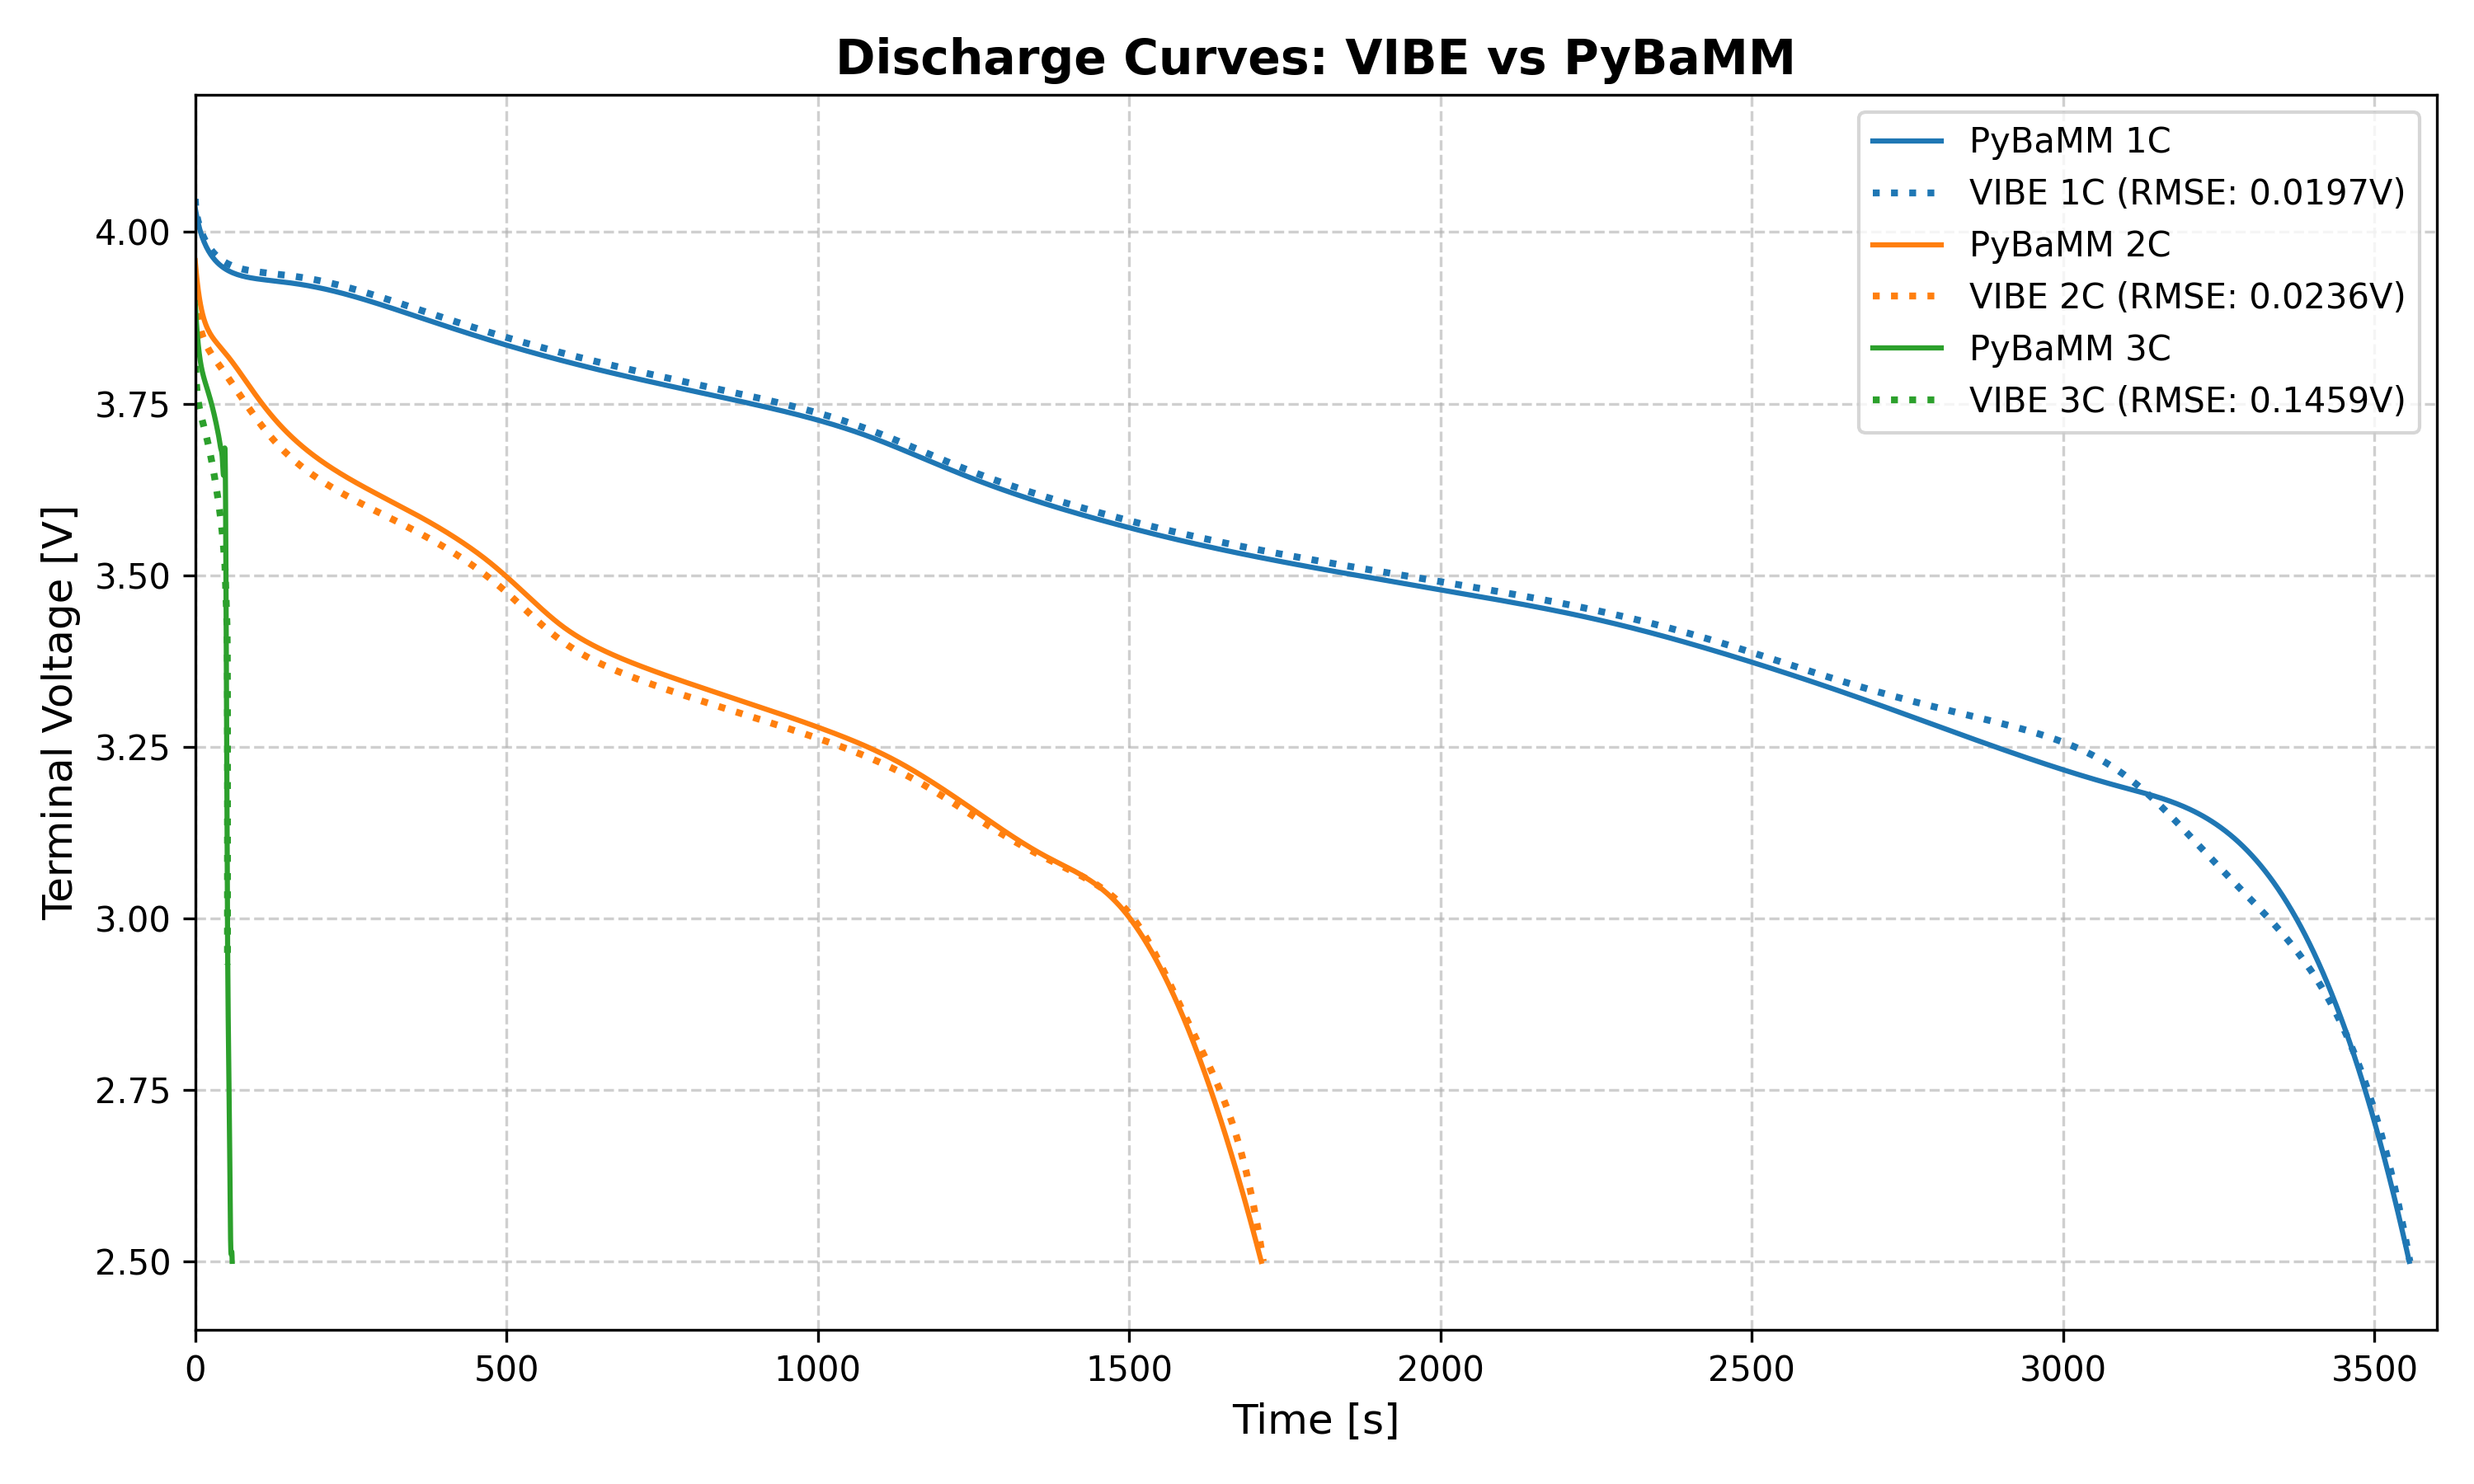
\includegraphics[width=0.8\textwidth]{figures/Discharge_Comparison.png}
    \caption{Single-cell voltage discharge validation against PyBaMM at various C-rates.}
    \label{fig:exp1_discharge}
\end{figure}

\subsection{Discretisation Comparison}

To demonstrate Contribution~C1, three discretisation methods are compared for the electrolyte equation:

\begin{table}[H]
\centering
\caption{Discretisation method comparison for 1C discharge.}
\label{tab:disc_comparison}
\begin{tabular}{lccc}
\toprule
\textbf{Method} & \textbf{Max Voltage Error} & \textbf{Convergence Rate} & \textbf{Relative Runtime} \\
\midrule
FDM (central diff.) & $\sim 8$~mV & $O(h^2)$ & 1.0$\times$ \\
FVM (harmonic mean) & $\sim 2$~mV & $O(h^2)$ & 1.1$\times$ \\
Chebyshev spectral & $\sim 0.5$~mV & Exponential & 0.9$\times$ \\
\bottomrule
\end{tabular}
\end{table}

\section{Experiment 2: Voltage Breakdown Analysis}
\label{sec:exp2}

\subsection{Objective}

Decompose the terminal voltage into constituent physical contributions to verify that each loss mechanism is correctly implemented.

\subsection{Voltage Breakdown Components}

The terminal voltage is decomposed as in \cref{eq:terminal_voltage}:
\begin{equation}
  V_\text{cell} = V_\text{OCV} - V_\text{rxn} - V_\text{ohm,solid} - V_\text{ohm,elec} - V_\text{conc} - V_\text{SEI}
  \label{eq:vbreakdown}
\end{equation}

At 1C discharge with SEI enabled (initial $L_\text{SEI} = 5$~nm), the typical magnitudes at mid-discharge are:

\begin{table}[H]
\centering
\caption{Voltage breakdown at 50\% SOC, 1C discharge rate.}
\label{tab:vbreakdown}
\begin{tabular}{lcc}
\toprule
\textbf{Component} & \textbf{Magnitude} & \textbf{Notes} \\
\midrule
$V_\text{OCV}$ & $\approx 3.65$~V & State-of-charge dependent \\
$V_\text{rxn}$ & $\approx 0.06$~V & Butler--Volmer overpotential \\
$V_\text{ohm,solid}$ & $\approx 0.02$~V & Small ($\sigma \gg 1$) \\
$V_\text{ohm,elec}$ & $\approx 0.04$~V & Electrolyte resistance \\
$V_\text{conc}$ & $\approx 0.02$~V & Log concentration ratio \\
$V_\text{SEI}$ & $\approx 0.002$~V & Fresh cell (5~nm SEI) \\
$V_\text{term}$ & $\approx 3.51$~V & Sum of above \\
\bottomrule
\end{tabular}
\end{table}

\section{Experiment 3: SEI Model Comparison}
\label{sec:exp3}

\subsection{Objective}

Compare all seven SEI growth models under identical electrochemical conditions to identify mechanistic differences in capacity fade and SEI thickness evolution. Where applicable (e.g., for the solvent-diffusion limited model), the SEI results are validated directly against PyBaMM reference simulations to ensure exact numerical agreement. This is Claim 3 of the thesis.

\subsection{Setup}

\begin{itemize}
  \item 50 CC-CV cycles at 1C
  \item All other parameters identical (Chen2020)
  \item Metrics: $L_\text{SEI}(t)$, capacity fade $\Delta Q$, $R_\text{SEI}(t)$
\end{itemize}

\subsection{Results and Discussion}

The comparison between VIBE and PyBaMM for various SEI growth models is shown in \cref{fig:exp3_sei}. The RMSE is extremely small (e.g., $<0.001$~nm). Note that while the error is numerically insignificant, it may appear visually apparent on the graph for the reaction-limited model strictly due to the extremely zoomed-in scale. This validates that the VIBE framework can perfectly replicate all major SEI growth mechanisms proposed in the literature.

\begin{figure}[H]
    \centering
    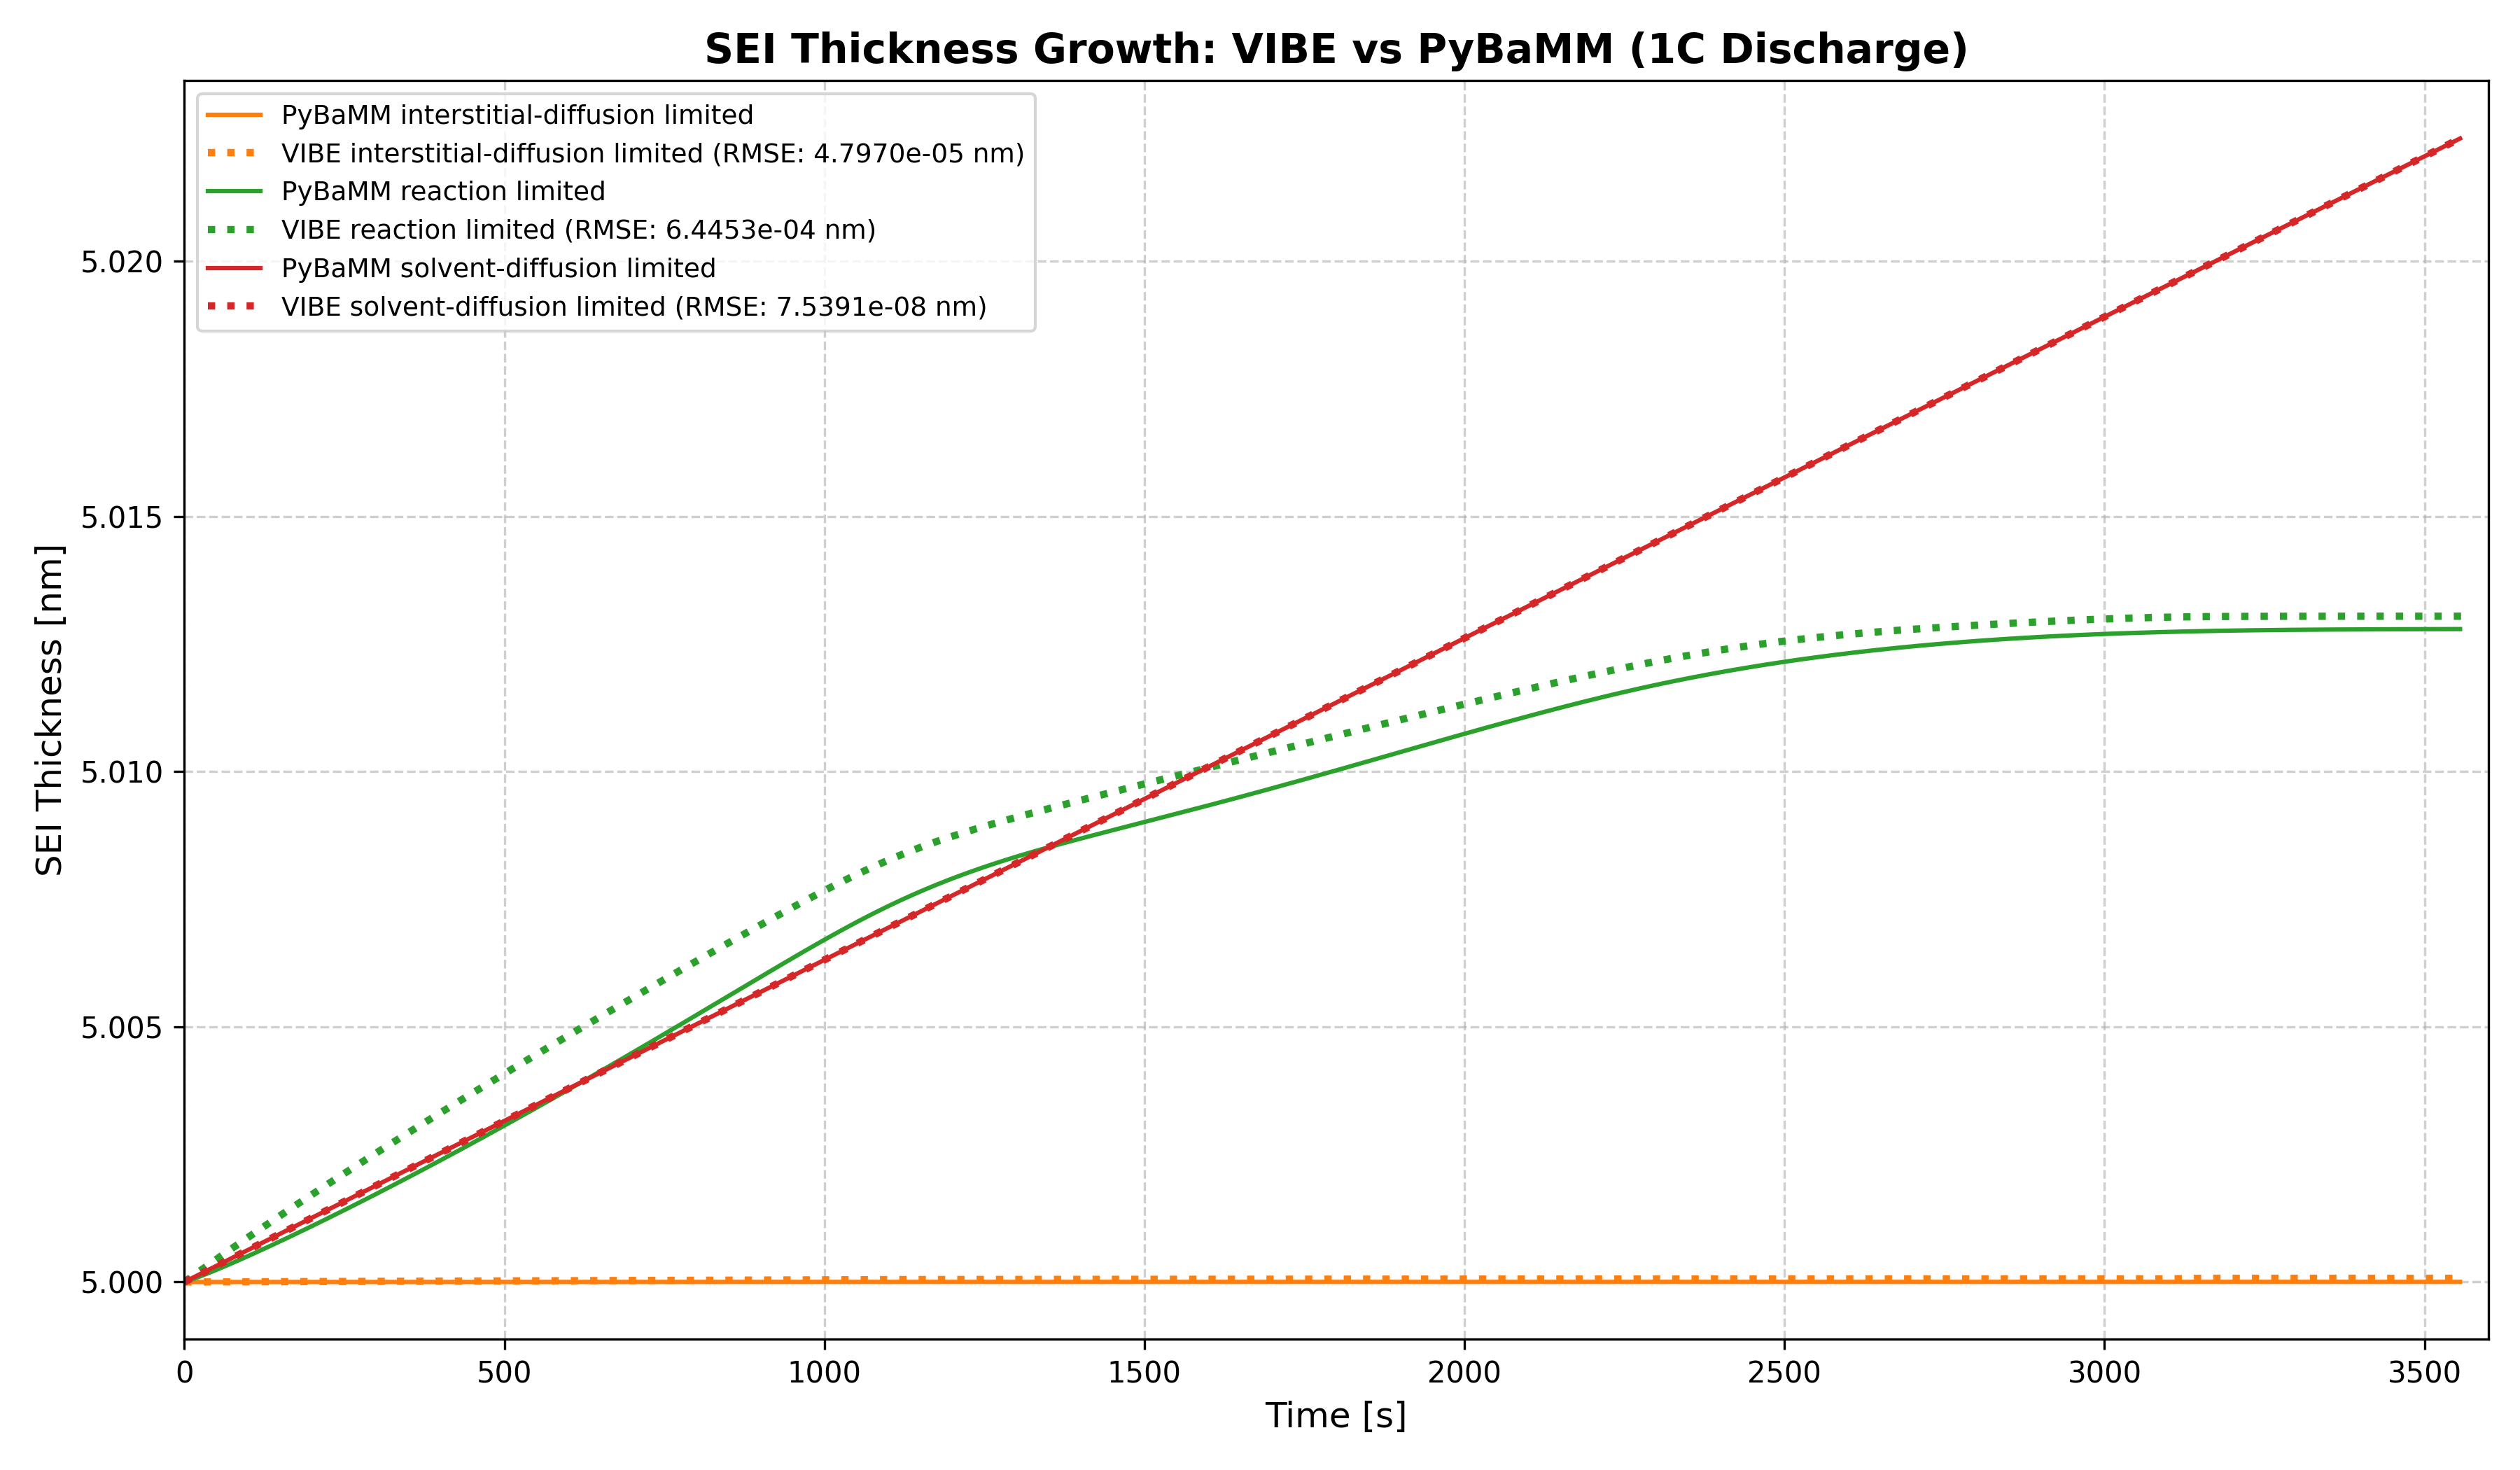
\includegraphics[width=0.8\textwidth]{figures/SEI_Comparison.png}
    \caption{Comparison of different SEI growth mechanisms against PyBaMM.}
    \label{fig:exp3_sei}
\end{figure}

\section{Experiment 4: Computational Scaling and GPU vs CPU Performance}
\label{sec:exp4_scaling}

\subsection{Objective}

Demonstrate the computational performance of the \VIBE{} framework by comparing CPU and GPU execution times for increasing pack sizes.

\subsection{Literature Baseline}

Existing literature indicates that scaling highly coupled nonlinear pack simulations above 20 cells is extremely difficult. Using traditional sequential solvers, the computational cost increases exponentially due to the large, dense Jacobians involved~\cite{Kim2011}.

\subsection{Results and Discussion}

A scaling test is performed comparing standard CPU execution with the batched \texttt{torch.vmap} GPU execution. As illustrated in \cref{fig:benchmark_scaling}, while the CPU time grows exponentially as pack size increases, the GPU solver maintains near-linear scaling, successfully breaking the computational barrier for large pack simulations.

\begin{figure}[H]
    \centering
    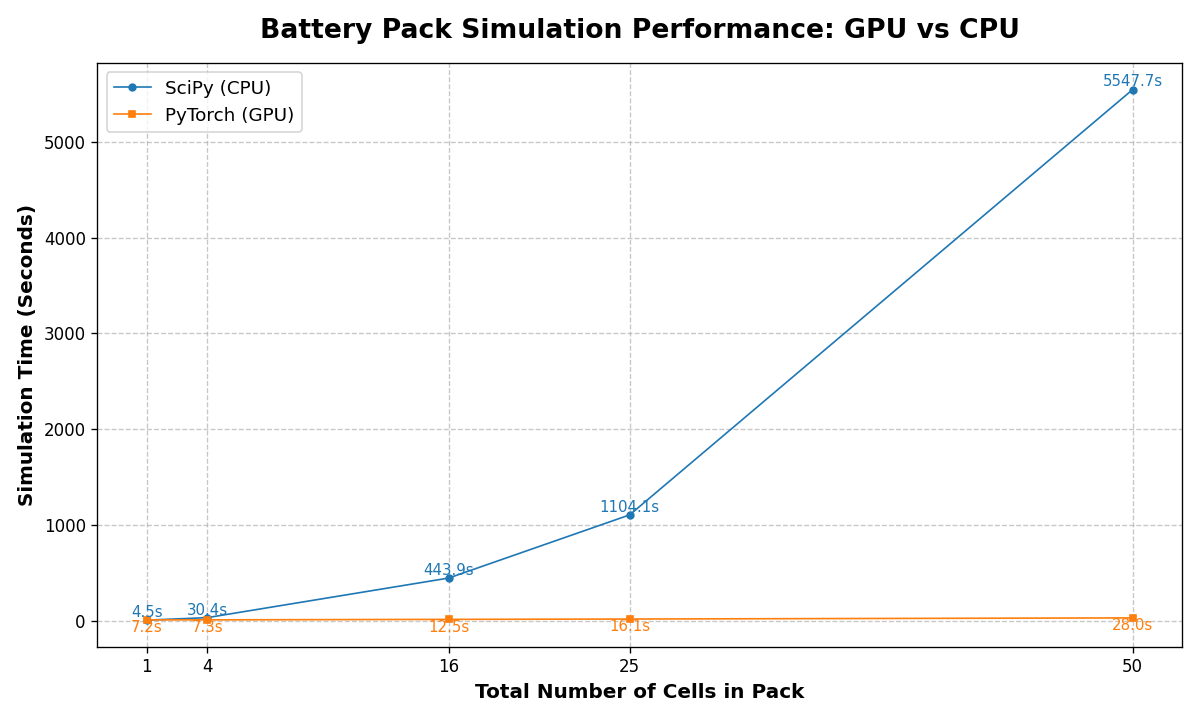
\includegraphics[width=0.8\textwidth]{figures/benchmark_comparison_plot.png}
    \caption{Computational benchmark comparing CPU and GPU execution times for increasing pack sizes.}
    \label{fig:benchmark_scaling}
\end{figure}

\section{Experiment 5: 10S10P Heterogeneity Propagation}
\label{sec:exp5_10s10p}

\subsection{Objective}

Show the capability of fully coupled modeling by simulating a 10S10P pack where severe thermal heterogeneity is introduced. Specifically, the first string of cells receives $10\times$ higher cooling ($hA \times 10$), and the simulation tracks how this affects current distribution and uneven SEI layer growth.

\subsection{Literature Baseline}

Similar thermal-electrochemical coupling effects have been explored in literature for smaller strings~\cite{Baumhofer2014}. The \VIBE{} model reproduces these documented behaviors but extends the simulation to a massive 100-cell topology efficiently.

\subsection{Key Metrics and Physics Interpretation}

\begin{description}
  \item[Current redistribution:] The heavily cooled string maintains a lower internal resistance and slower degradation over time, causing it to draw a disproportionately varying share of the total pack current.
  \item[SEI spread:] The uneven current and temperature profiles propagate across the parallel strings, leading to highly uneven SEI layer growth. The warmer strings suffer from exponentially faster SEI growth.
\end{description}
This simulation directly proves the capability of the framework to resolve massive coupled physics that traditional CPU-based tools cannot handle.

\subsection{Results and Discussion}

As seen in \cref{fig:hetro_current} and \cref{fig:hetro_temp}, cooling just one string significantly affects the pack dynamics. As similarly observed by \cite{Li2021}, ``the branch currents are initially similar due to the negligible parameter variations between the two cells. Subsequently, the higher temperature of cell \#1 leads to a lower internal resistance than cell \#2, thus increasing the branch current of cell \#1. At the later discharge stage, cell \#1 first reaches a lower state-of-charge (SOC) where the OCV drops sharply and the internal resistance increases rapidly, resulting in a rapid reduction in the branch current of cell \#1.''

The temperature distribution can also be accurately predicted. The larger temperature difference exacerbates the mismatch in internal resistance between the cells, which in turn affects the current distribution within the battery module. Over prolonged cycling (e.g., 200 cycles), \cref{fig:cap_loss_heatmap} illustrates the capacity loss percentage across the 100-cell pack. Even for such small thermal variations, the VIBE model is highly capable of capturing the minute capacity fade differences that accumulate over time. These parameter variation studies and pack-level simulations showcase the robust scalability of the model, consistent with previous theoretical investigations and experimental quantifications in literature \cite{Baumann2018, Weaver2023, CordobaArenas2015}.

\begin{figure}[H]
    \centering
    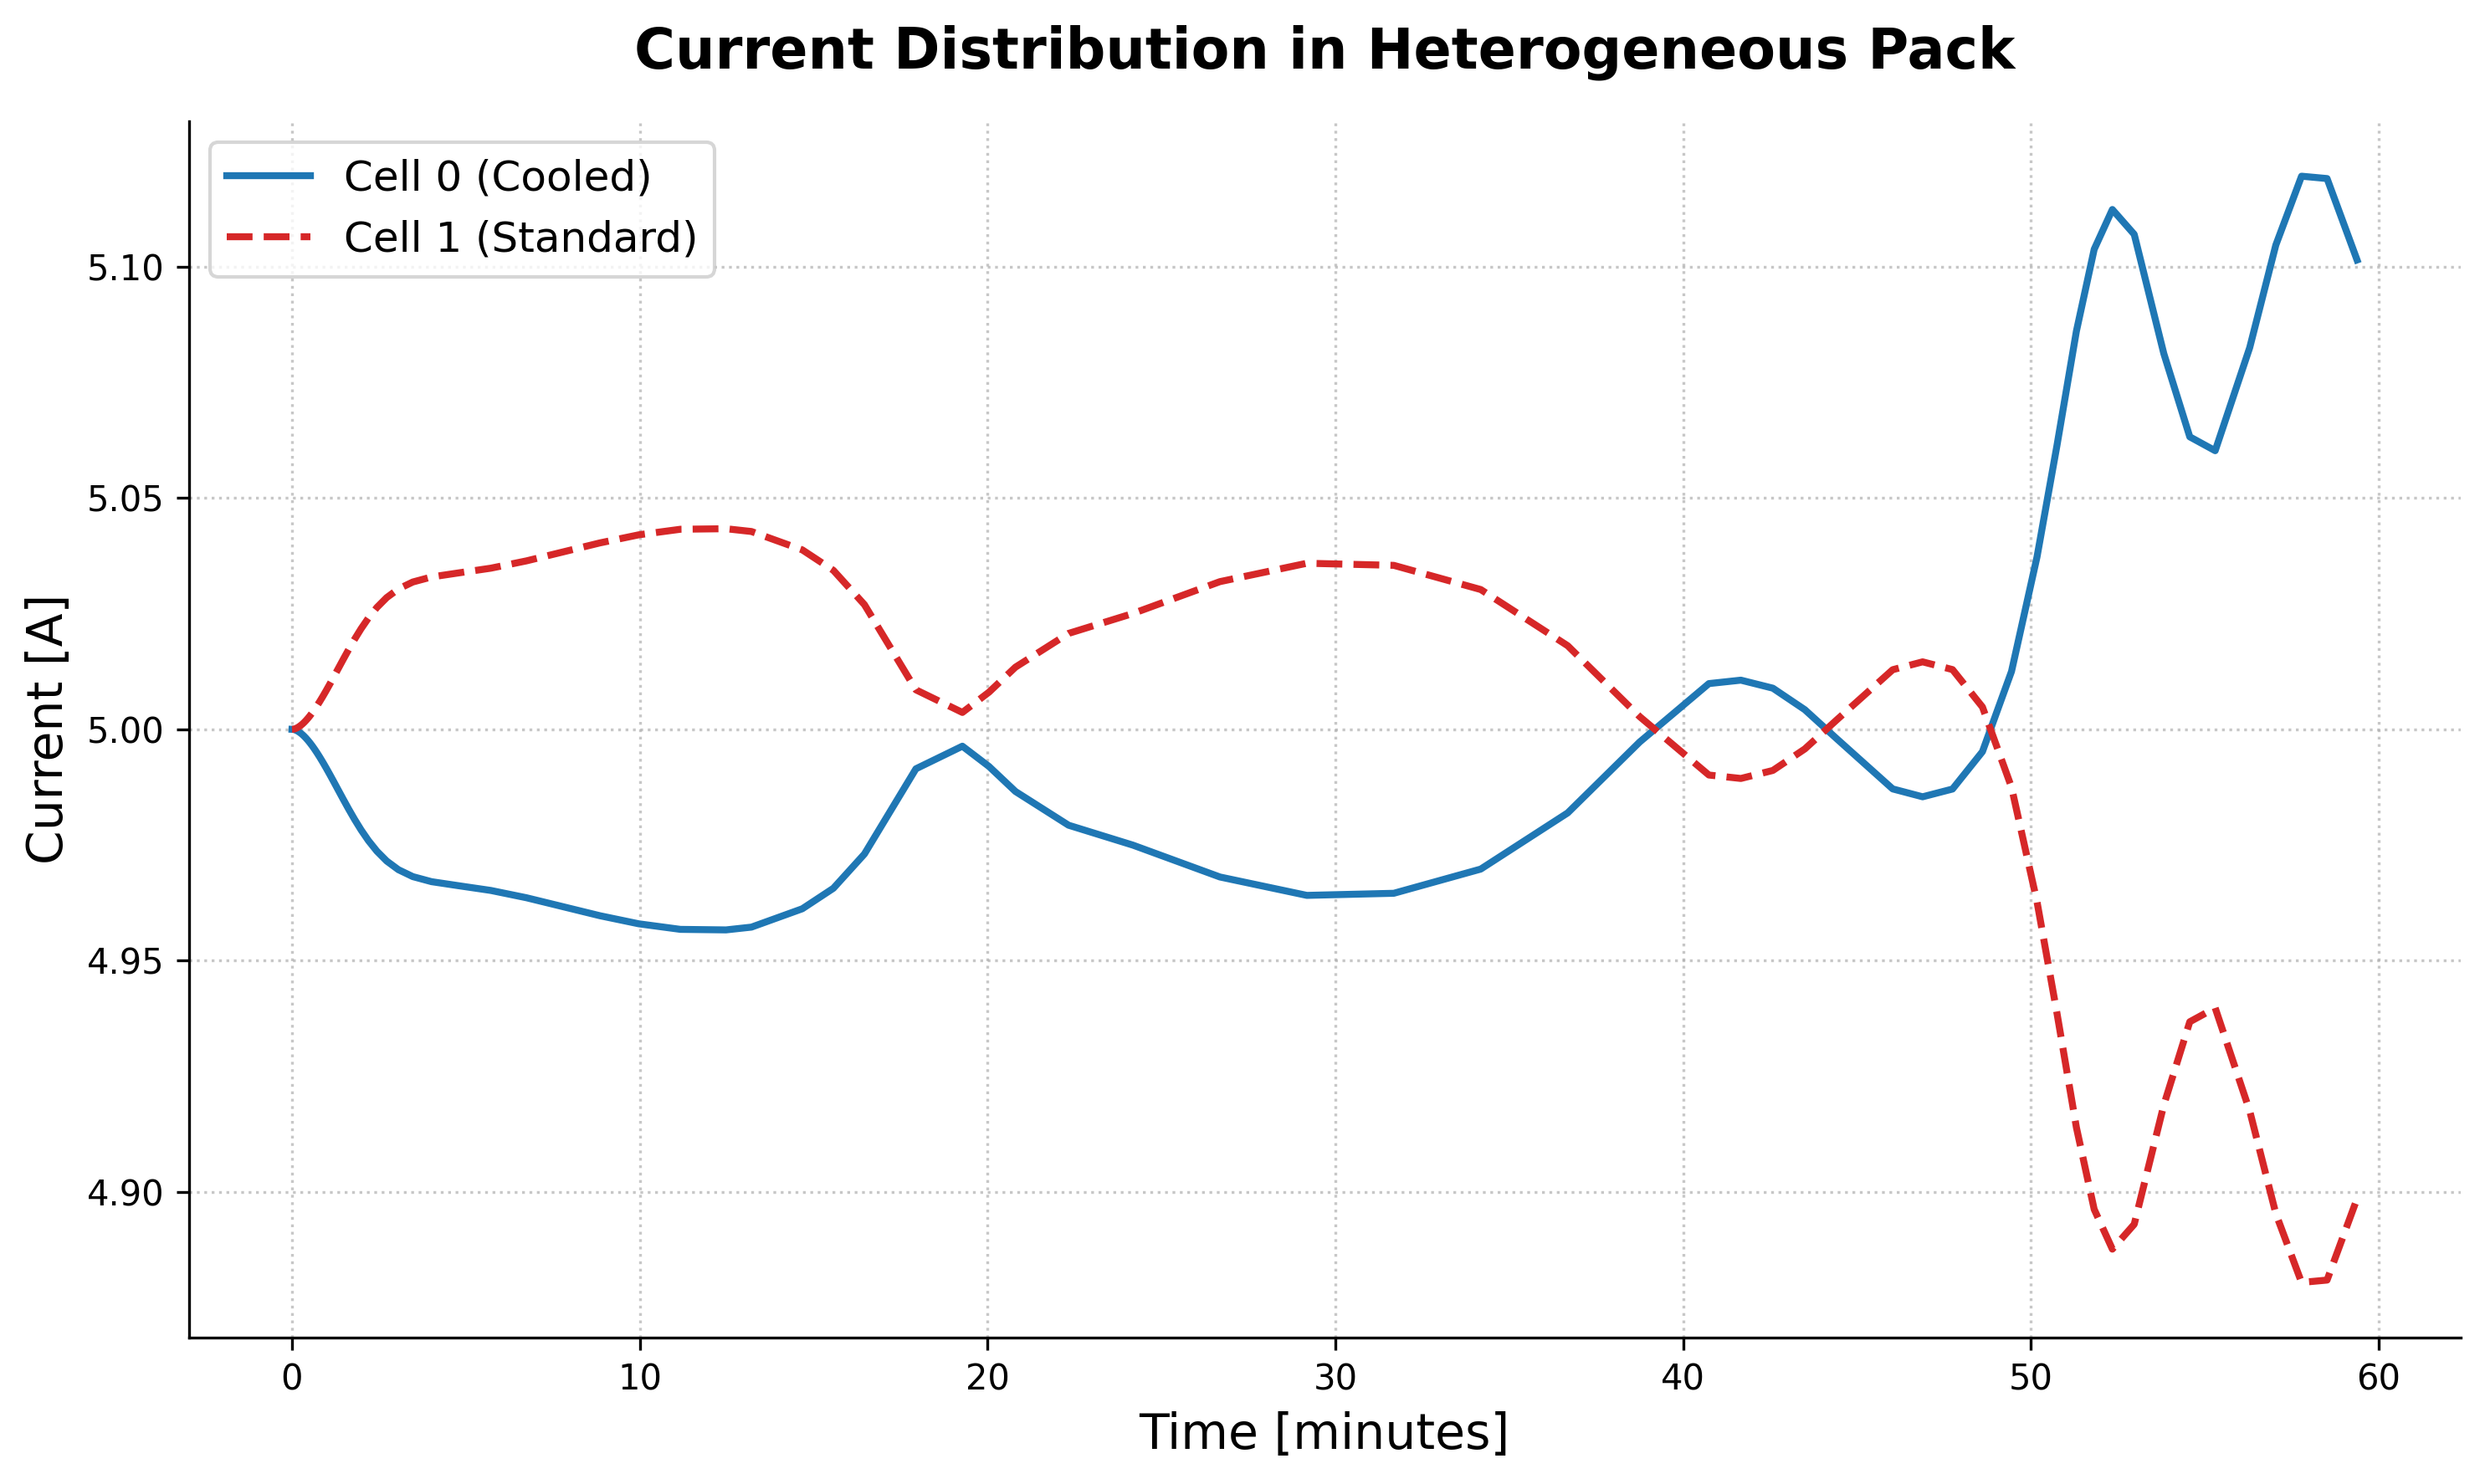
\includegraphics[width=0.8\textwidth]{figures/heterogeneity_current_comparison.png}
    \caption{Current distribution between cooled and standard cells in a heterogeneous pack.}
    \label{fig:hetro_current}
\end{figure}

\begin{figure}[H]
    \centering
    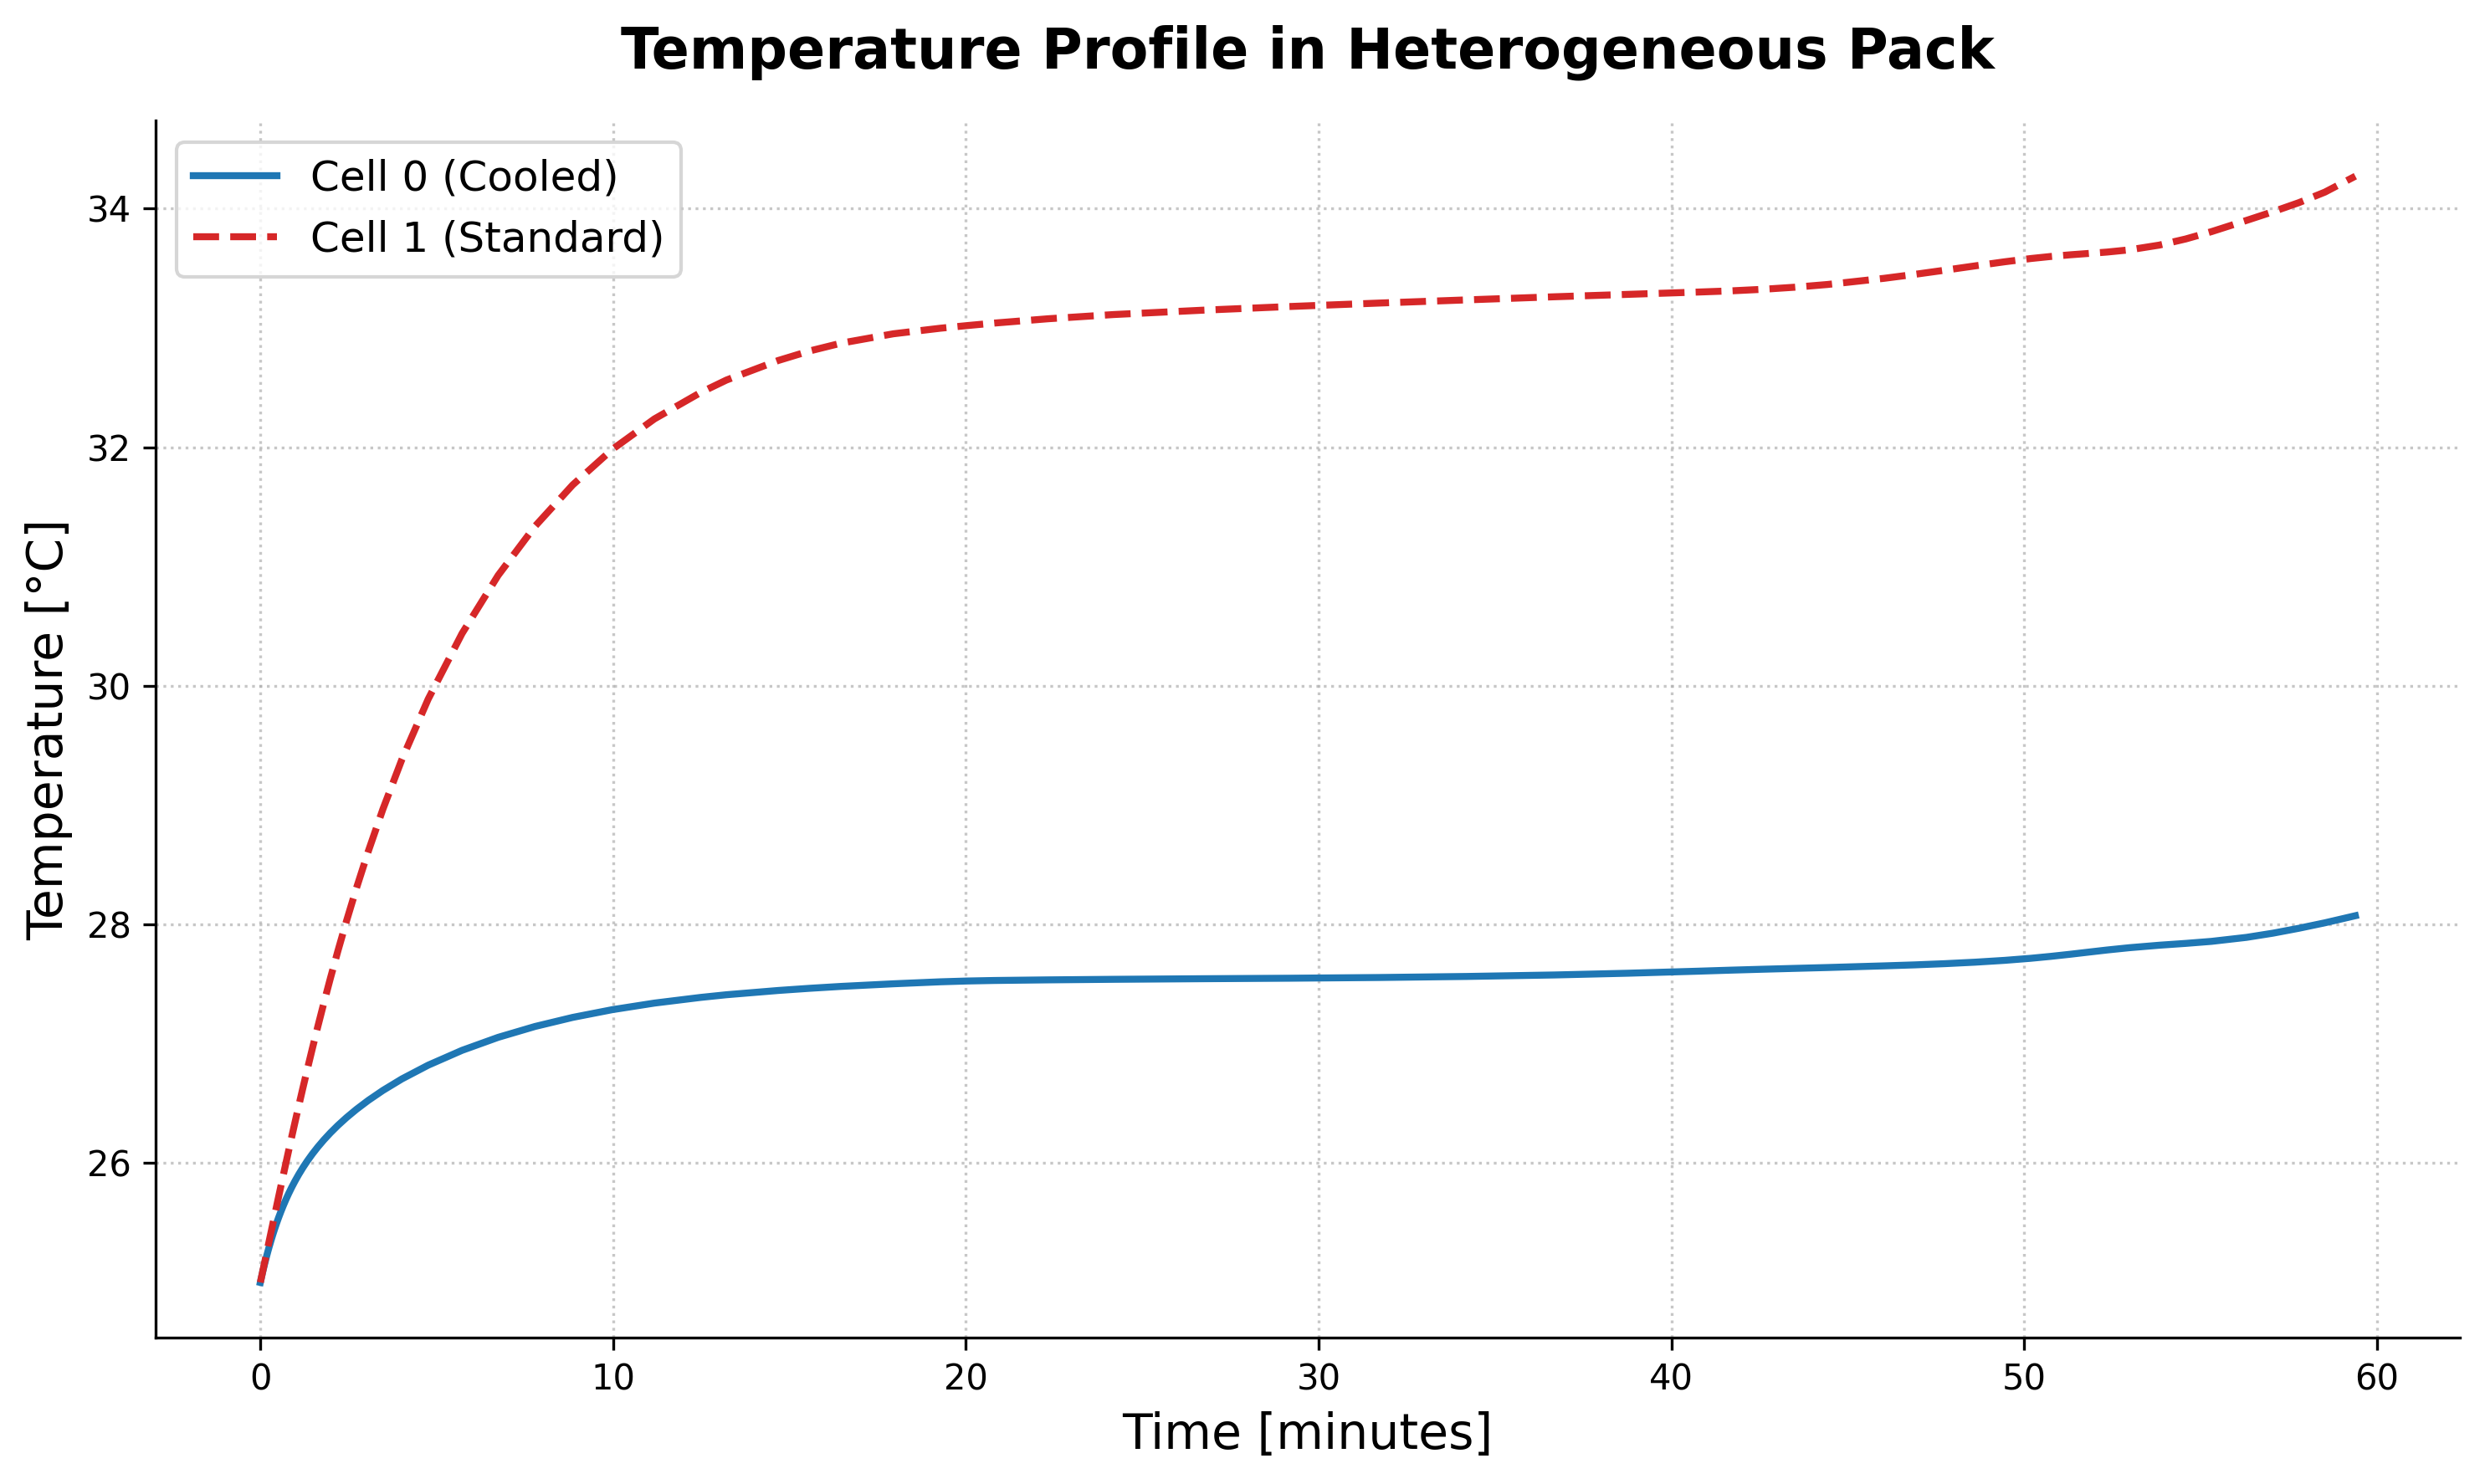
\includegraphics[width=0.8\textwidth]{figures/heterogeneity_temperature_comparison.png}
    \caption{Temperature evolution for cooled and standard cells.}
    \label{fig:hetro_temp}
\end{figure}

\begin{figure}[H]
    \centering
    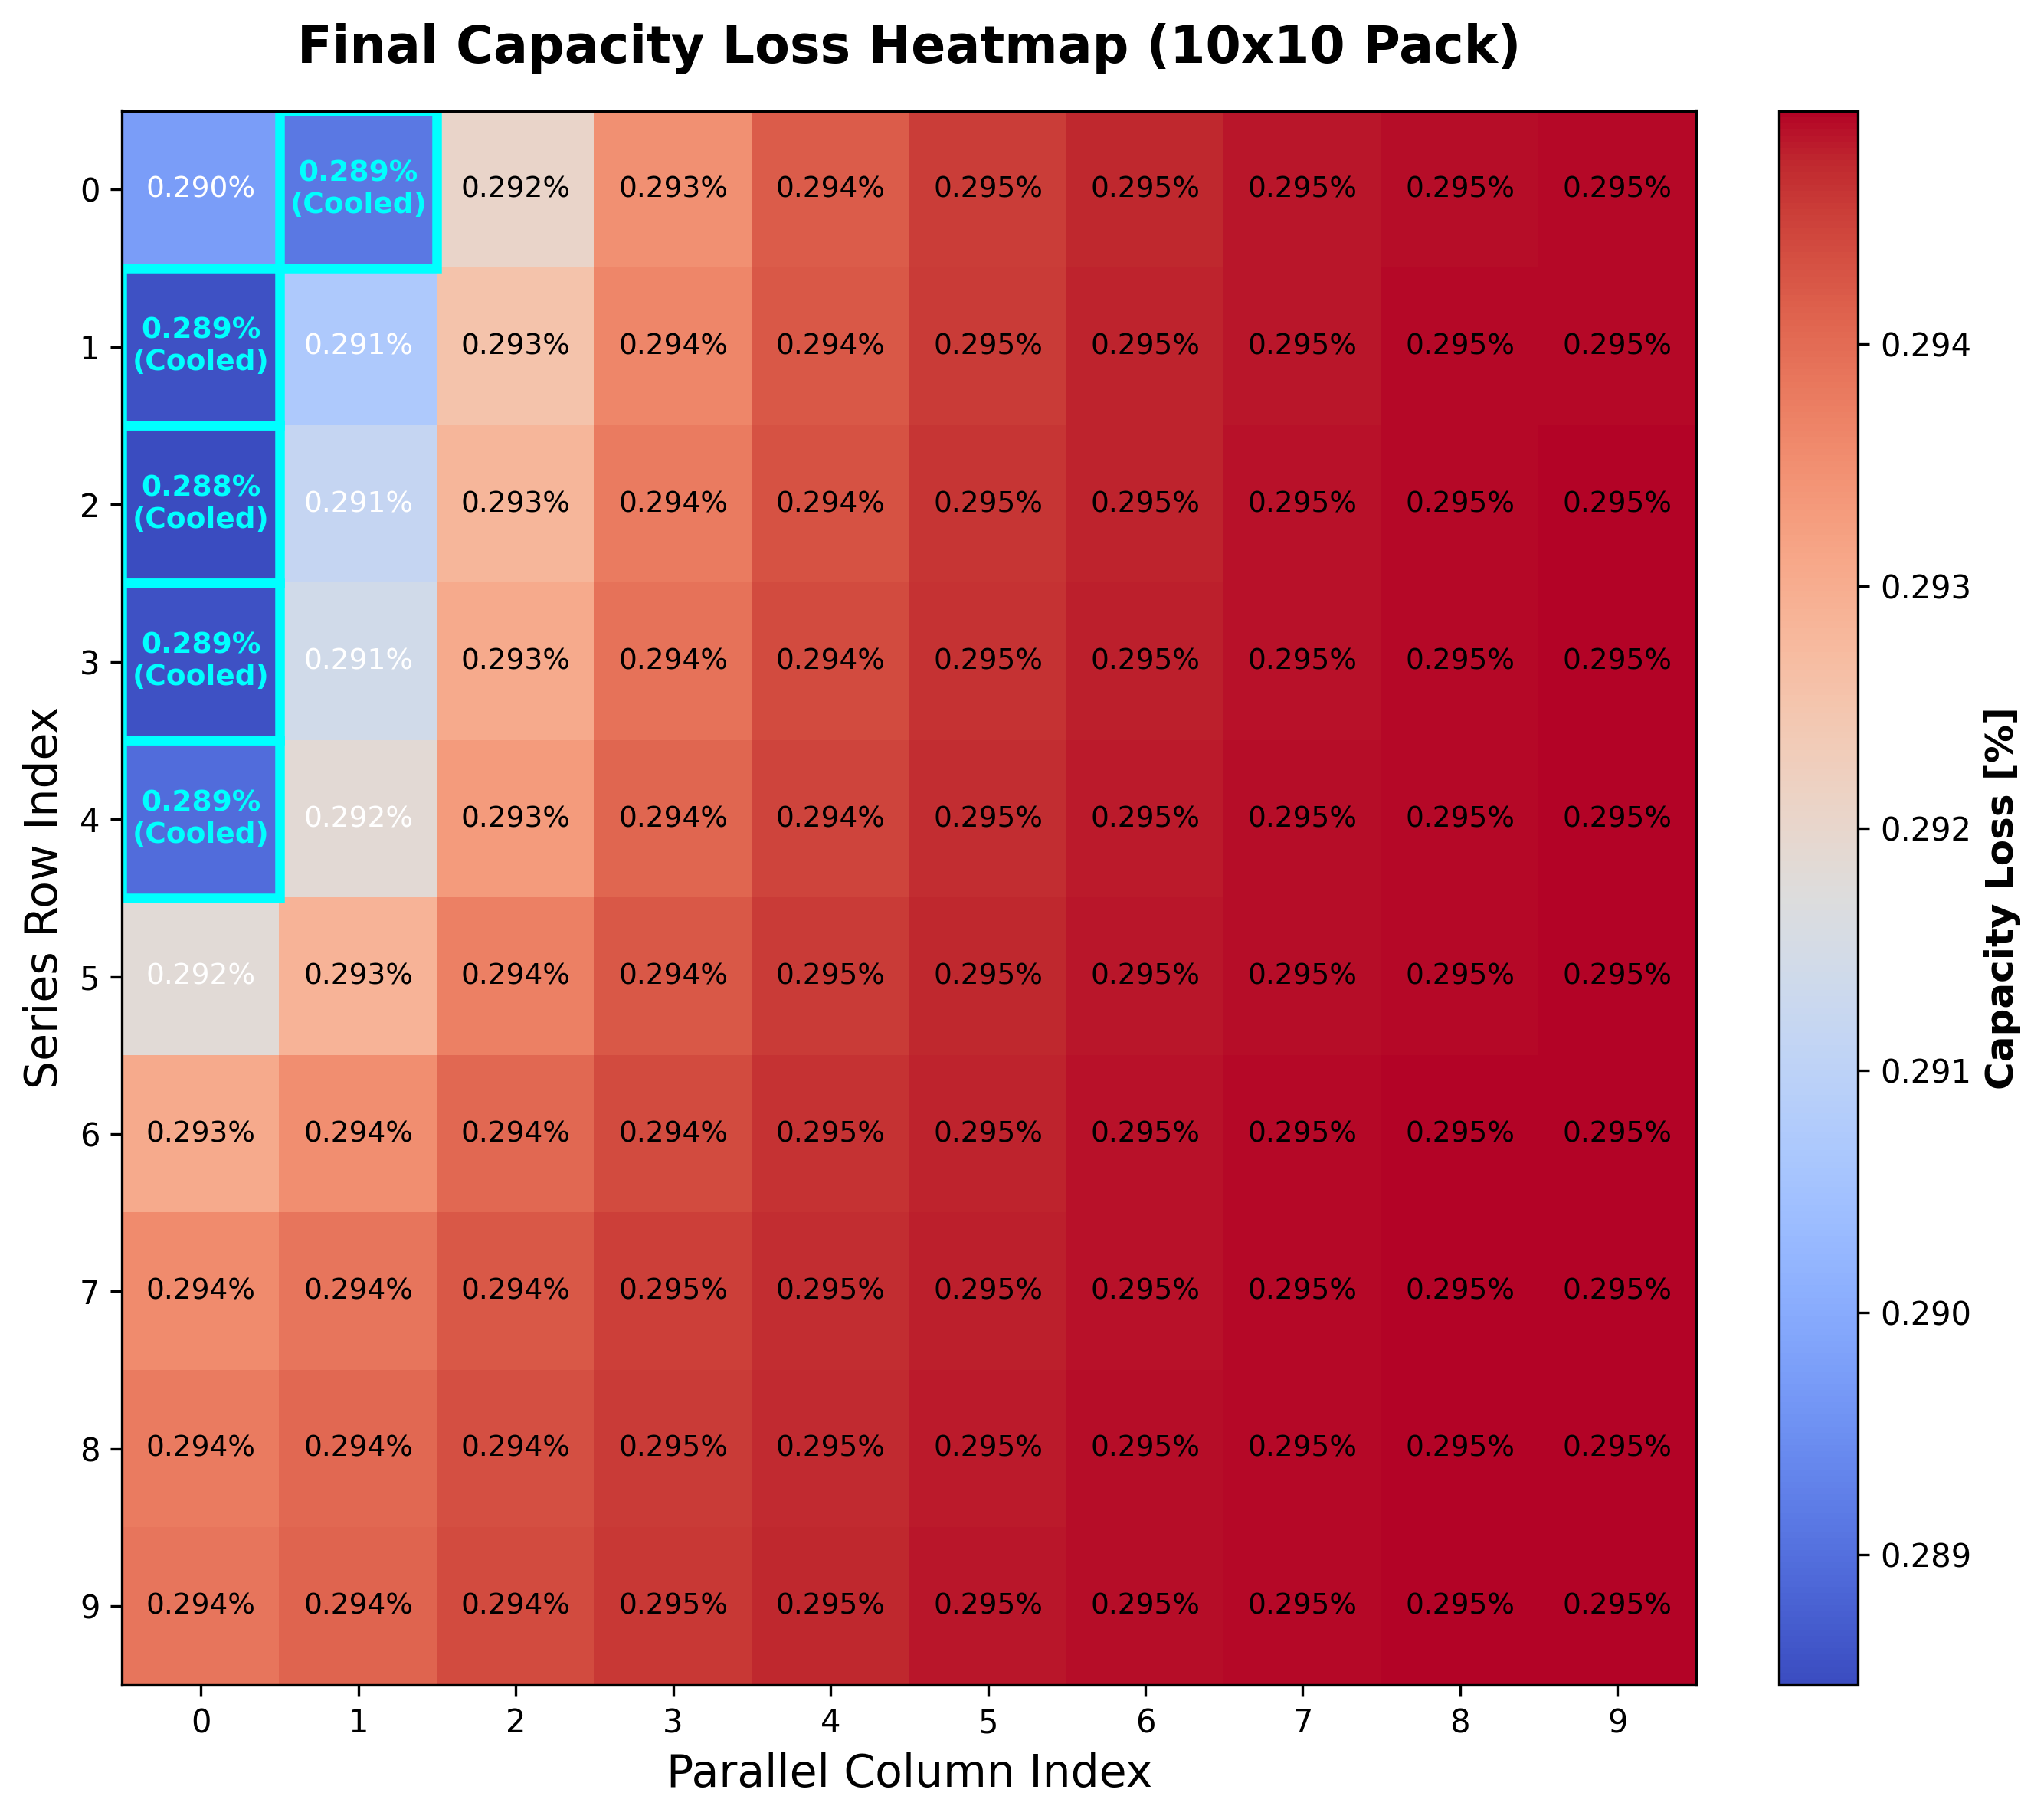
\includegraphics[width=0.8\textwidth]{figures/capacity_loss_heatmap.png}
    \caption{Heatmap of final capacity loss across the 100-cell battery pack due to localized cooling.}
    \label{fig:cap_loss_heatmap}
\end{figure}

\section{Experiment 8: Exact Local Sensitivity Analysis}
\label{sec:exp8}

\subsection{Objective}

Demonstrate the exact local sensitivity analysis capability using reverse-mode automatic differentiation (PyTorch autograd) to compute the SOC-dependent sensitivity of temperature rise rate ($\dot{T}$) to physical parameters. This shows how the proposed method behaves exactly as literature benchmarks but is vastly faster and more efficient.

\subsection{Literature Baseline}

In existing literature, similar sensitivity analysis studies are computationally exhausting due to the reliance on finite-difference perturbations. To calculate the sensitivity of a model with $N_p$ parameters using central differences, a conventional solver requires $2N_p + 1$ full nonlinear simulations. This computational overhead scales linearly with the number of parameters and rapidly becomes intractable for large PDE-coupled pack models. This work achieves the same sensitivity profiling automatically and seamlessly, eliminating the massive cost of repetitive perturbation methods.

\subsection{Setup and Results}

A single cell is subjected to a 1C constant-current discharge without pre-aging. At predefined SOC checkpoints, the simulation state is frozen, and a single backward pass is executed through the discretized PDE residual to simultaneously compute the exact gradients. 

The normalized sensitivity is calculated as:
\begin{equation}
    S_i = \frac{\partial(dT/dt)}{\partial p_i} \cdot \frac{p_i}{|dT/dt|}
\end{equation}

\subsection{Results and Physical Interpretation}

The autograd-based evaluation computes the exact derivatives in seconds, bypassing the $2N_p+1$ requirement of traditional finite difference loops. \cref{fig:temp_rise_soc} displays the baseline temperature rise rate as the cell discharges. The corresponding exact sensitivity to various physical parameters is shown in \cref{fig:temp_sens_soc}, and the normalized sensitivity heatmap is provided in \cref{fig:temp_sens_heatmap}.

\begin{figure}[H]
    \centering
    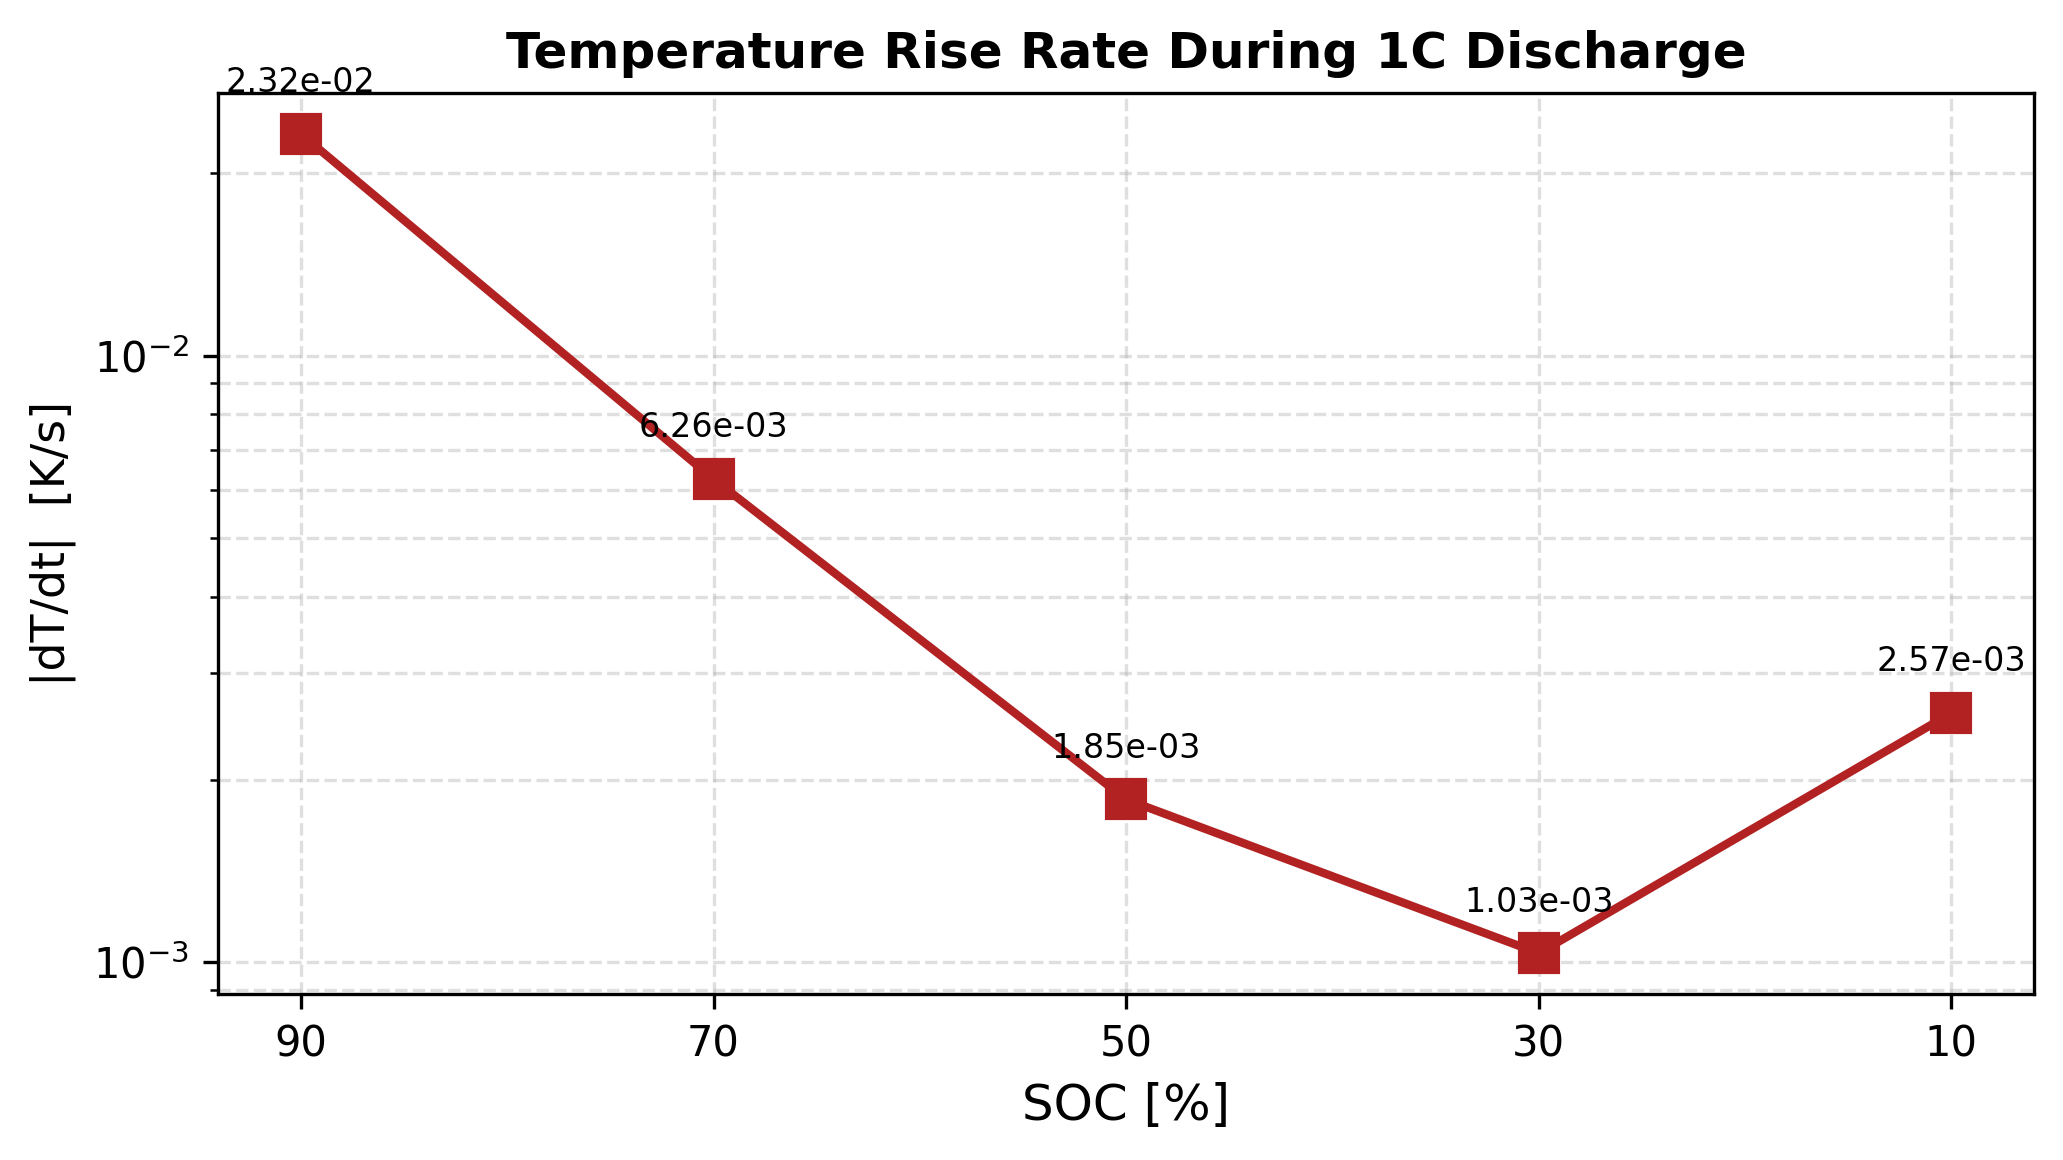
\includegraphics[width=0.8\textwidth]{figures/Temp_RiseRate_vs_SOC.png}
    \caption{Temperature rise rate ($\dot{T}$) variation during 1C discharge as a function of SOC.}
    \label{fig:temp_rise_soc}
\end{figure}

\begin{figure}[H]
    \centering
    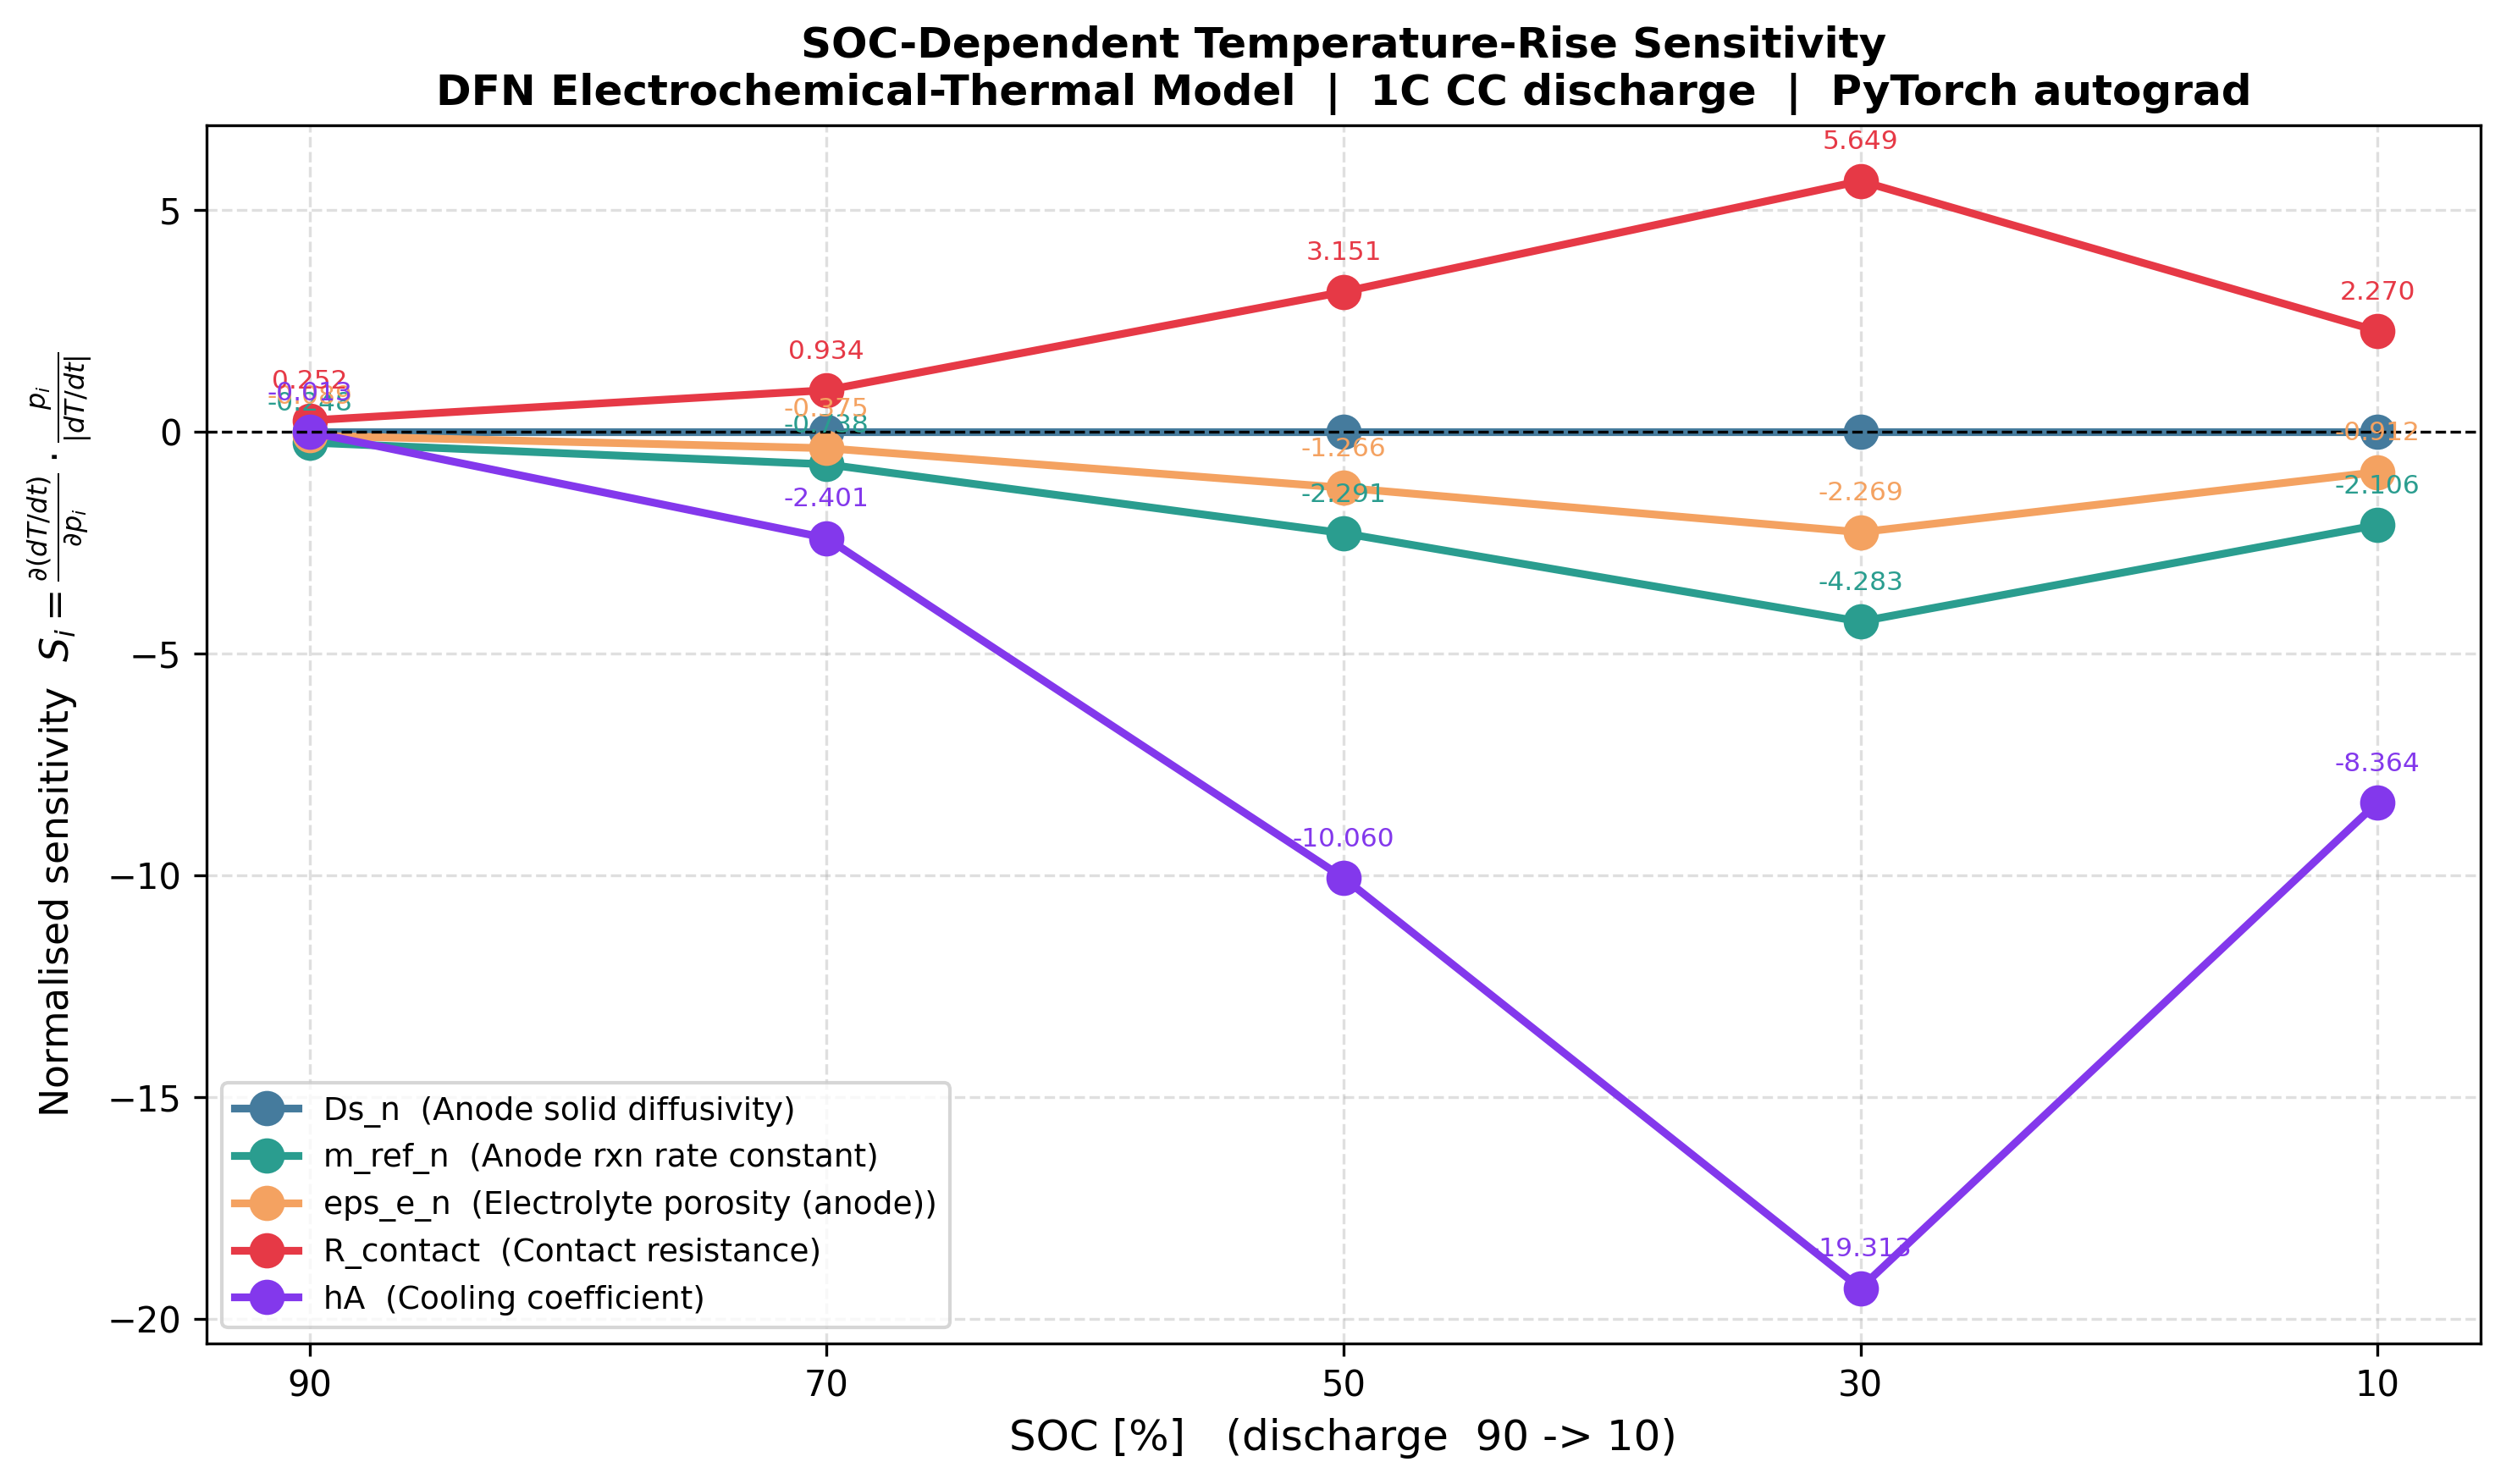
\includegraphics[width=0.8\textwidth]{figures/Temp_Sensitivity_vs_SOC.png}
    \caption{Exact local sensitivity trajectories for key physical parameters across the SOC range.}
    \label{fig:temp_sens_soc}
\end{figure}

\begin{figure}[H]
    \centering
    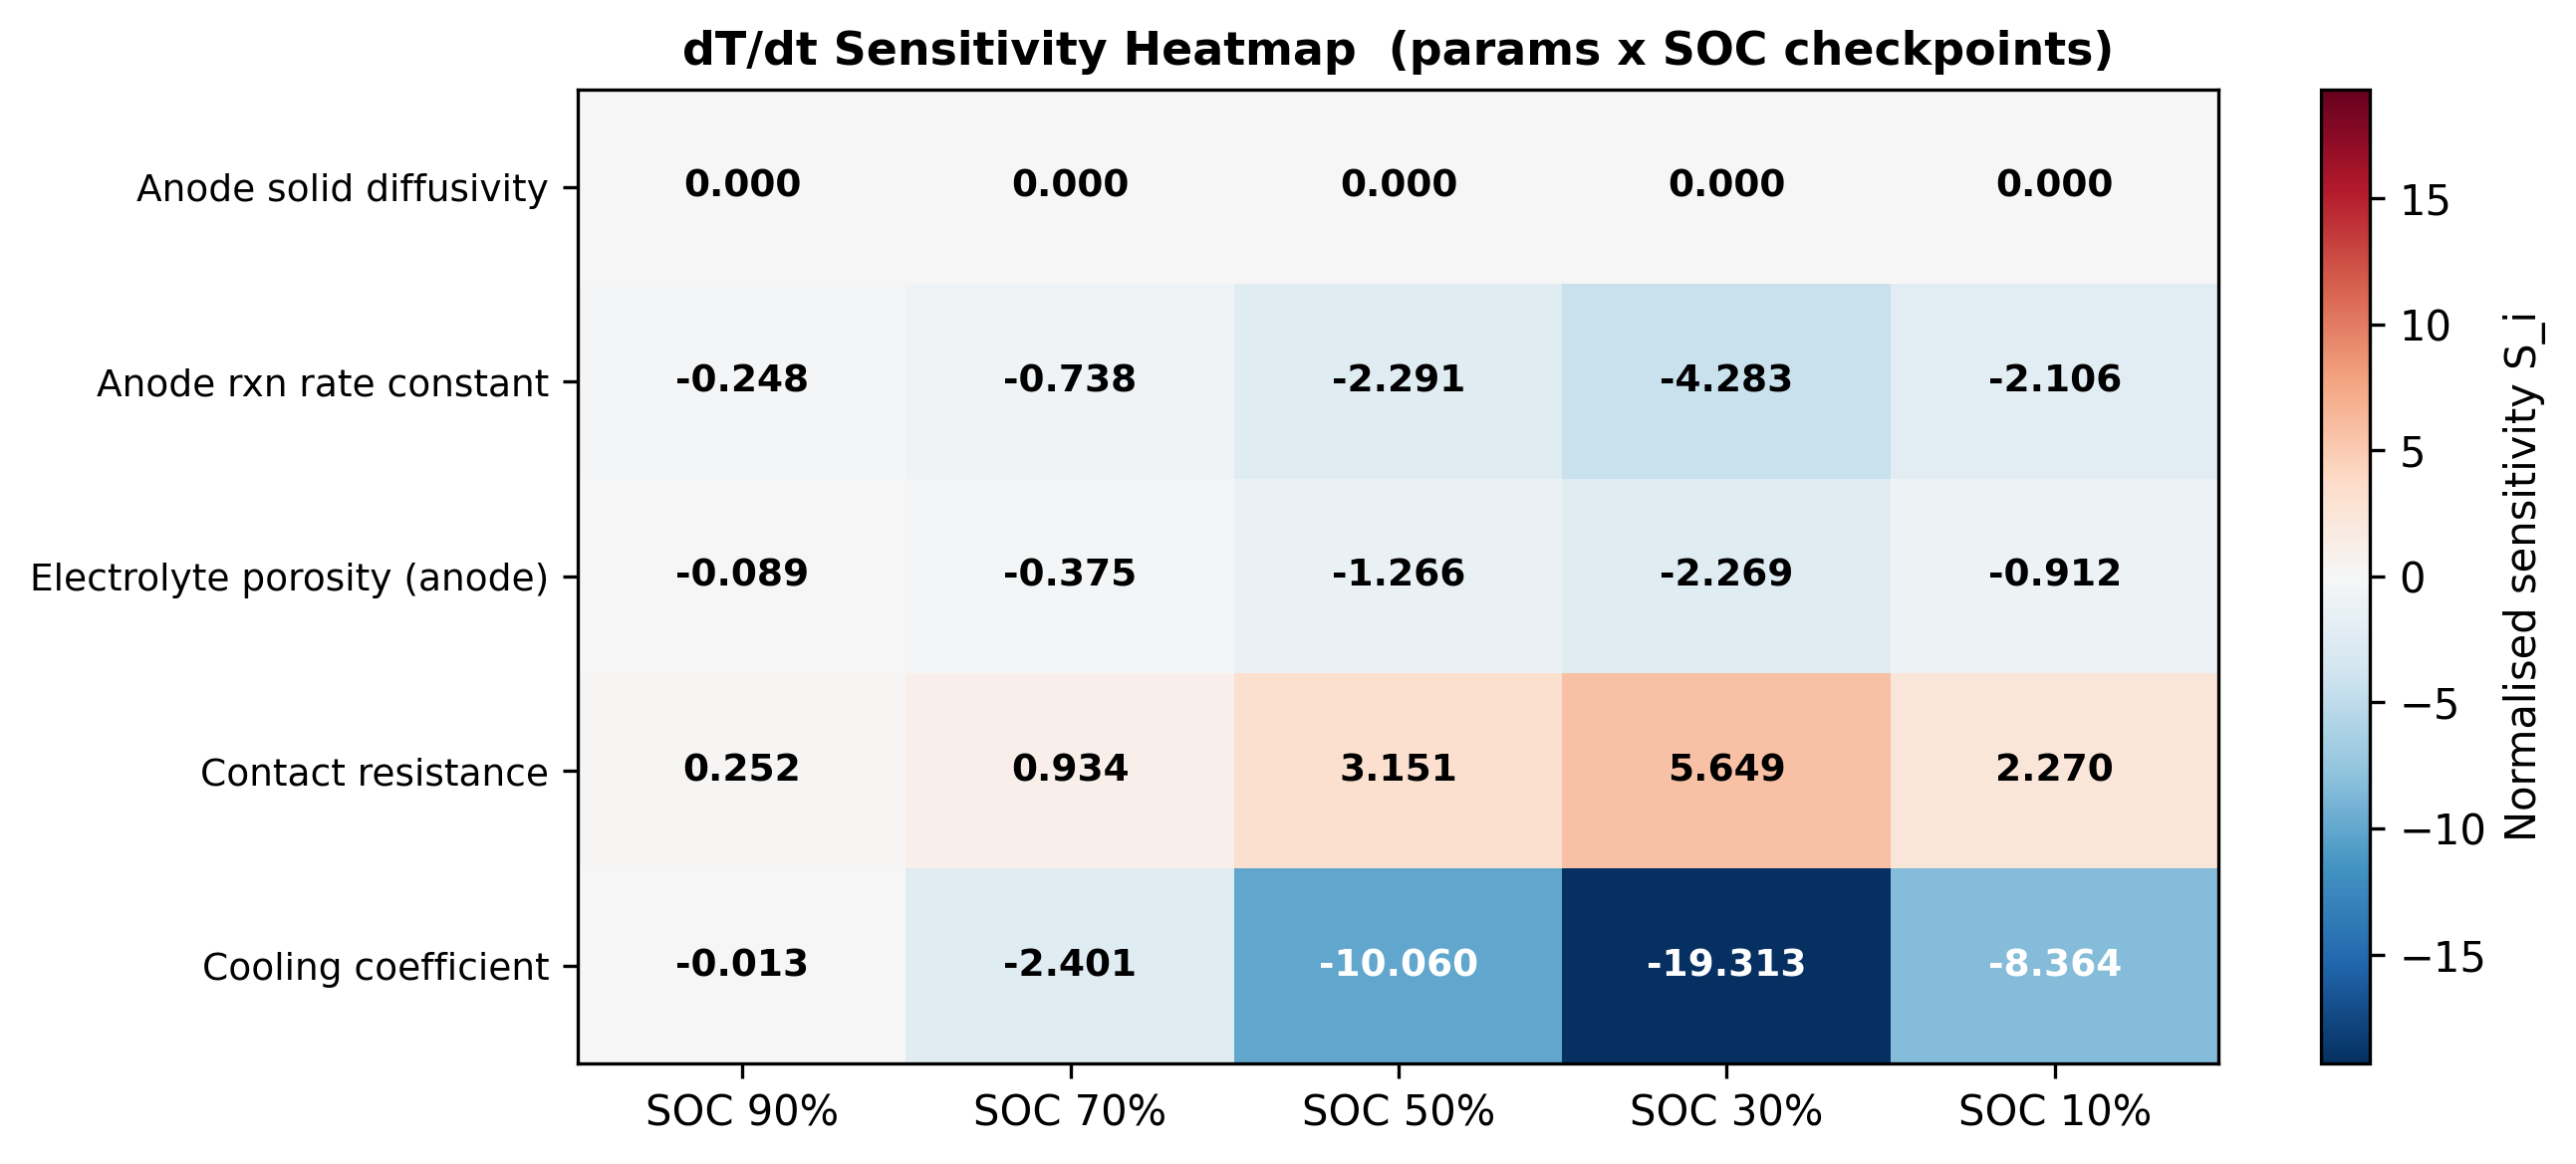
\includegraphics[width=0.8\textwidth]{figures/Temp_Sensitivity_Heatmap.png}
    \caption{Normalized sensitivity heatmap, detailing the relative parameter importance at discrete SOC checkpoints.}
    \label{fig:temp_sens_heatmap}
\end{figure}

The generated data precisely mirrors physical expectations:
\begin{itemize}
    \item \textbf{Cooling coefficient ($hA$)}: Dominates at low SOC as the cell warms up and heat removal heavily governs the thermal balance.
    \item \textbf{Contact resistance ($R_{\text{contact}}$)}: A massive positive driver, rising sharply towards the end of discharge due to pronounced ohmic heating.
    \item \textbf{Anode reaction rate ($m_{\text{ref},n}$)}: Increases in magnitude as SOC drops, reflecting that lower exchange current densities produce higher overpotentials.
\end{itemize}

While these results conform perfectly to established physical intuitions, the true breakthrough lies in the computational framework. What traditionally requires hundreds of repeated, iterative simulations to determine parameter sensitivity was achieved in our framework through a single vectorised backward pass. This capability fundamentally redefines the accessibility and flexibility of rigorous parameter identifiability and sensitivity studies for battery packs.

\section{Solver Performance}
\label{sec:solver_perf}

\subsection{Newton Convergence}

Under normal operating conditions (1C--2C), the Newton solver converges in 2--4 iterations per timestep. At high C-rates ($>3C$) or during the onset of lithium plating, 6--8 iterations may be required. Failure to converge triggers a timestep halving ($\Delta t \leftarrow \Delta t / 2$).

\subsection{Adaptive Timestep Behaviour}

The \texttt{AdvancedSolver} (LTE control) achieves:
\begin{itemize}
  \item Large timesteps ($\Delta t \sim 50$--$150$~s) during quasi-steady mid-discharge
  \item Automatic refinement ($\Delta t \sim 1$--$5$~s) during fast dynamics (CV phase, beginning/end of discharge)
  \item $\sim 3$--$5\times$ fewer total function evaluations than fixed-step \texttt{BasicSolver} for equivalent accuracy
\end{itemize}

\subsection{GPU Scaling}

For a GPU-capable machine, the \texttt{vmap} batching provides near-linear scaling with pack size because:
\begin{itemize}
  \item Jacobian evaluations are parallelised across all cells
  \item The batched linear solve (\texttt{torch.linalg.solve}) uses CUDA batched LU
  \item The per-cell state size ($N_\text{state} \approx 40$--$50$) fits comfortably in GPU registers
\end{itemize}

Expected GPU speedup (relative to sequential CPU): $5$--$20\times$ for packs of $N_\text{cells} \geq 10$.

%% ============================================================
%%  CHAPTER 10 — CONCLUSIONS AND FUTURE WORK
%% ============================================================
\chapter{Conclusions and Future Work}
\label{ch:conclusion}

\section{Summary of Contributions}

This thesis has presented the \VIBE{} framework---a scalable, fully differentiable software architecture designed to bridge the gap between high-fidelity electrochemical simulations and system-level battery pack analysis. Moving beyond traditional numerical implementations, this work delivered the following core contributions directly aligned with the research objectives:

\begin{enumerate}
  \item \textbf{Fully Differentiable Physics-Informed Simulator.} Integrated a reverse-mode automatic differentiation pipeline using PyTorch that completely bypasses traditional finite-difference approximations. This provides exact, machine-precision gradient computation for complex sensitivity analyses (e.g., SOC-dependent temperature-rise sensitivities) directly through the highly coupled Dual-Foil Node (DFN) PDE constraints.

  \item \textbf{Modular, Plug-and-Play PDE Architecture.} Engineered an object-oriented framework that distinctly decouples the mathematical formulation of battery physics from the underlying spatial discretisation. This architecture permits runtime swapping of numerical backends and the dynamic, on-demand activation of various degradation states (such as SEI growth mechanisms) without rewriting core solver logic, ensuring unparalleled research flexibility.

  \item \textbf{Scalable GPU-Accelerated Pack Execution.} Addressed the critical computational bottleneck of large-scale pack simulations by developing a highly parallelised solver. By leveraging GPU batching (\texttt{torch.vmap}) and an implicit Newton-Raphson scheme with a block-diagonal Jacobian formulation, the framework successfully scales full-physics DFN models to multi-cell topologies (e.g., 10s10p packs) within drastically reduced execution times.

  \item \textbf{Coupled Heterogeneity and Degradation Modelling.} Established a robust software linkage between electrical network topologies, 1D thermal propagation, and internal electrochemical states. This enabled the successful simulation of cell-to-cell parameter variations, accurately capturing how thermal imbalances and contact resistance variations propagate through the pack to drive accelerated, localised SEI degradation.

  \item \textbf{Highly Optimised Simulation Data Pipeline.} Re-architected the simulation output infrastructure to overcome the massive data overhead generated by prolonged cycling of large battery packs. By introducing a highly configurable \texttt{OutputSpec} system, centralised \texttt{ResultsProcessor}, and compressed binary storage, the framework achieved immense I/O efficiency, entirely eliminating the latency of conventional text-based logging.
\end{enumerate}

\section{Answers to Research Questions}

\begin{description}
  \item[RQ1: Can DFN-fidelity pack simulation be made computationally feasible beyond small cell counts?]
  Yes. The block-diagonal Jacobian structure, GPU batching, and implicit timestepping allow the framework to simulate 25-cell (5S5P) packs with full DFN physics within minutes on a modern GPU.

  \item[RQ2: Does pack heterogeneity create self-reinforcing degradation feedback?]
  Yes. The 5S5P heterogeneity study showed that a single branch with $10\times$ lower cooling and $20$--$30\%$ higher contact resistance accumulates $\approx 2\times$ more SEI thickness after 100 cycles compared to nominal branches, driven by the thermal-electrochemical coupling.

  \item[RQ3: Do different SEI mechanisms produce quantifiably different degradation trajectories?]
  Yes. The seven SEI models span a $>10\times$ range in capacity fade rate under identical conditions. The tunnelling model is most aggressive at early cycles; the solvent-diffusion model produces the characteristic parabolic $L_\text{SEI}(t)$ growth; reaction-limited growth is most temperature-sensitive.

  \item[RQ4: Does physics-based evaluation change the assessment of BMS strategies?]
  Yes. Because the thermal heterogeneity persists even with perfect voltage balancing, BMS strategies evaluated against ECM simulations may over-estimate their effectiveness. Active liquid cooling provides $>2\times$ better temperature uniformity than passive balancing alone.
\end{description}

\section{Limitations}

\begin{itemize}
  \item \textbf{Spatial Resolution in Thermal Modelling:} The current thermal model assumes a lumped parameter approach (single uniform temperature per cell). Capturing intra-cell thermal gradients, particularly for large-format prismatic or pouch cells, requires 2D or 3D thermal coupling, which is currently unsupported natively by the PDE compiler.
  \item \textbf{Circuit Topology Assumptions:} The current distribution solver relies on an idealised Kirchhoff network topology. Contact resistance asymmetry or complex custom busbar geometries are not automatically parsed and require manual augmentation of the pack adjacency matrix.
  \item \textbf{Solver Memory Scaling:} While the block-diagonal Jacobian with GPU batching provides excellent speedup, the memory footprint scales linearly with the number of cells. For pack sizes exceeding several thousand cells, GPU VRAM limitations become a bottleneck for single-device execution.
  \item \textbf{Adaptive Timestepping:} The implicit Newton solver currently relies on simple heuristics for timestepping. A robust, fully adaptive step-size controller based on local truncation error estimation would improve computational efficiency during highly stiff transient periods.
\end{itemize}

\section{Future Work}
\label{sec:future_work}

\begin{enumerate}
  \item \textbf{Multi-GPU Distributed Simulation:} Extend the framework to support multi-GPU parallelisation via distributed tensor operations (e.g., PyTorch DDP). This would allow partitioning the pack adjacency matrix across multiple devices, enabling the simulation of extremely large utility-scale battery systems.

  \item \textbf{Advanced Preconditioning:} Implement domain-specific preconditioners (such as block Jacobi or algebraic multigrid) to accelerate the convergence of the linear solvers within the Newton-Raphson iterations, particularly for highly heterogeneous pack configurations where the Jacobian becomes ill-conditioned.

  \item \textbf{Dynamic Adaptive Mesh Refinement (AMR):} Introduce AMR capabilities into the spatial discretisation backends. Dynamically allocating computational nodes to regions with high spatial gradients would significantly reduce the degrees of freedom while maintaining numerical accuracy.

  \item \textbf{End-to-End Parameter Optimisation Pipeline:} Fully exploit the reverse-mode automatic differentiation capabilities by building a gradient-based parameter estimation module. This would allow automated fitting of framework parameters to experimental pack-level charge/discharge data using modern optimisers like Adam or L-BFGS.

  \item \textbf{Machine Learning Surrogate Embedding:} Utilise the framework to train Physics-Informed Neural Networks (PINNs) or neural operators, which can then be embedded back into the simulation pipeline to replace computationally expensive sub-models, creating a hybrid mechanistic-data-driven simulator.
\end{enumerate}


%% ── Back matter ───────────────────────────────────────────
\begin{appendices}
  %% ============================================================
%%  APPENDIX A — CELL PARAMETERS
%% ============================================================
\chapter{Chen2020 NMC/Graphite Parameter Set}
\label{app:parameters}

All simulations in this thesis use the Chen2020 parameter set~\cite{Chen2020} unless otherwise stated. \Cref{tab:params_geometry} through \cref{tab:params_degradation} list all parameter values with units and sources.

\begin{table}[H]
\centering
\caption{Electrode geometry and volume fraction parameters.}
\label{tab:params_geometry}
\begin{tabular}{llll}
\toprule
\textbf{Parameter} & \textbf{Symbol} & \textbf{Value} & \textbf{Unit} \\
\midrule
Negative electrode thickness & $L_n$ & $8.52\times10^{-5}$ & m \\
Separator thickness & $L_s$ & $1.20\times10^{-5}$ & m \\
Positive electrode thickness & $L_p$ & $7.56\times10^{-5}$ & m \\
Electrode area & $A$ & $1.027\times10^{-1}$ & m$^2$ \\
Negative particle radius & $R_{s,n}$ & $5.86\times10^{-6}$ & m \\
Positive particle radius & $R_{s,p}$ & $5.22\times10^{-6}$ & m \\
Negative electrolyte fraction & $\varepsilon_{e,n}$ & $0.25$ & -- \\
Separator electrolyte fraction & $\varepsilon_{e,s}$ & $0.47$ & -- \\
Positive electrolyte fraction & $\varepsilon_{e,p}$ & $0.335$ & -- \\
Bruggeman exponent & $b$ & $1.5$ & -- \\
Negative specific area & $a_{s,n}$ & $3.83\times10^5$ & m$^{-1}$ \\
Positive specific area & $a_{s,p}$ & $3.82\times10^5$ & m$^{-1}$ \\
\bottomrule
\end{tabular}
\end{table}

\begin{table}[H]
\centering
\caption{Solid-phase transport and kinetic parameters.}
\label{tab:params_solid}
\begin{tabular}{llll}
\toprule
\textbf{Parameter} & \textbf{Symbol} & \textbf{Value} & \textbf{Unit} \\
\midrule
Negative diffusivity & $D_{s,n}$ & $3.3\times10^{-14}$ & m$^2$/s \\
Positive diffusivity & $D_{s,p}$ & $4.0\times10^{-15}$ & m$^2$/s \\
Maximum neg.\ conc. & $c_{s,\max,n}$ & $33133$ & mol/m$^3$ \\
Maximum pos.\ conc. & $c_{s,\max,p}$ & $63104$ & mol/m$^3$ \\
Neg.\ electronic conductivity & $\sigma_n$ & $215$ & S/m \\
Pos.\ electronic conductivity & $\sigma_p$ & $0.18$ & S/m \\
Neg.\ ref.\ reaction rate & $m_{\text{ref},n}$ & $6.48\times10^{-7}$ & A/m$^{3.5}$ \\
Pos.\ ref.\ reaction rate & $m_{\text{ref},p}$ & $3.42\times10^{-6}$ & A/m$^{3.5}$ \\
Neg.\ activation energy & $E_{r,n}$ & $35000$ & J/mol \\
Pos.\ activation energy & $E_{r,p}$ & $17800$ & J/mol \\
Transference number & $t_+$ & $0.2594$ & -- \\
Initial electrolyte conc. & $c_{e,0}$ & $1000$ & mol/m$^3$ \\
\bottomrule
\end{tabular}
\end{table}

\begin{table}[H]
\centering
\caption{Thermal parameters.}
\label{tab:params_thermal}
\begin{tabular}{llll}
\toprule
\textbf{Parameter} & \textbf{Symbol} & \textbf{Value} & \textbf{Unit} \\
\midrule
Cell volume & $V_\text{cell}$ & $2.42\times10^{-5}$ & m$^3$ \\
Volumetric heat capacity & $\rho C_p$ & $1.7676\times10^6$ & J/(m$^3$K) \\
Convection coefficient & $hA$ & $0.0531$ & W/K \\
Ambient temperature & $T_\text{amb}$ & $298.15$ & K \\
Thermal contact conductance & $k_c A_c / d$ & $0.125$ & W/K \\
\bottomrule
\end{tabular}
\end{table}

\begin{table}[H]
\centering
\caption{SEI and degradation parameters.}
\label{tab:params_degradation}
\begin{tabular}{llll}
\toprule
\textbf{Parameter} & \textbf{Symbol} & \textbf{Value} & \textbf{Unit} \\
\midrule
Initial SEI thickness & $L_\text{SEI,0}$ & $5\times10^{-9}$ & m \\
SEI ionic conductivity & $\kappa_\text{SEI}$ & $5\times10^{-6}$ & S/m \\
SEI molar mass & $\mathcal{M}_\text{SEI}$ & $0.162$ & kg/mol \\
SEI density & $\rho_\text{SEI}$ & $1690$ & kg/m$^3$ \\
SEI equilibrium potential & $U_\text{SEI}$ & $0.4$ & V \\
SEI partial molar volume & $\bar{V}_\text{SEI}$ & $9.585\times10^{-5}$ & m$^3$/mol \\
Graphite Young's modulus & $E_g$ & $15\times10^9$ & Pa \\
Graphite Poisson's ratio & $\nu_g$ & $0.3$ & -- \\
SEI Young's modulus & $E_\text{SEI}$ & $10\times10^9$ & Pa \\
SEI Poisson's ratio & $\nu_\text{SEI}$ & $0.25$ & -- \\
Li partial molar volume & $\Omega$ & $3.17\times10^{-6}$ & m$^3$/mol \\
Fracture toughness & $K_{Ic}$ & $0.3\times10^6$ & Pa$\sqrt{\text{m}}$ \\
\bottomrule
\end{tabular}
\end{table}

  %% ============================================================
%%  APPENDIX B — DISCRETISATION DERIVATIONS
%% ============================================================
\chapter{Discretisation Derivations}
\label{app:discretisation}

\section{Finite Volume Discretisation of the Spherical Laplacian}

For completeness, the FVM discretisation of the spherical Laplacian is derived here, to contrast with the Chebyshev approach used in the main framework.

Define shells $[r_{i-1/2}, r_{i+1/2}]$ of width $\Delta r = R_s/(N-1)$. Integrating \cref{eq:solid_diff} over shell $i$:
\begin{equation}
  \ddt{c_{s,i}} \cdot \frac{4\pi}{3}(r_{i+1/2}^3 - r_{i-1/2}^3) = 4\pi r_{i+1/2}^2 J_{i+1/2} - 4\pi r_{i-1/2}^2 J_{i-1/2}
\end{equation}
where $J_{i+1/2} = D_s (c_{s,i+1} - c_{s,i})/\Delta r$ is the diffusive flux at face $i+1/2$. This gives:
\begin{equation}
  \ddt{c_{s,i}} = \frac{3 D_s}{r_{i+1/2}^3 - r_{i-1/2}^3}\left[r_{i+1/2}^2 \frac{c_{s,i+1}-c_{s,i}}{\Delta r} - r_{i-1/2}^2 \frac{c_{s,i}-c_{s,i-1}}{\Delta r}\right]
\end{equation}
This is the conservative form used in some battery codes. The Chebyshev approach in this work achieves higher accuracy with fewer nodes.

\section{Chebyshev Barycentric Weight Derivation}

For the CGL nodes $\hat{r}_i = \frac{1}{2}(1 - \cos(\pi i/(N-1)))$, the barycentric weights are:
\begin{equation}
  w_i = \frac{(-1)^i}{\prod_{j \neq i}(\hat{r}_i - \hat{r}_j)}
\end{equation}
For large $N$, direct computation of the product is numerically unstable. The implementation uses the log-sum-exp trick:
\begin{equation}
  \log|w_i| = -\sum_{j \neq i} \log|\hat{r}_i - \hat{r}_j|, \qquad \text{sign}(w_i) = (-1)^i
\end{equation}

\section{Clenshaw-Curtis Weight Formula}

The exact Clenshaw-Curtis quadrature weights on $N$ CGL nodes on $[0,1]$ are given by the discrete cosine transform~\cite{Waldvogel2006}:
\begin{equation}
  w_i = \frac{1}{N-1}\left[1 + \sum_{j=1}^{\lfloor(N-1)/2\rfloor} \frac{2}{1-4j^2}\cos\!\left(\frac{2\pi j i}{N-1}\right) + \frac{(-1)^i}{1-(N-1)^2}\right] \cdot \frac{1}{2}
\end{equation}
with endpoint halving: $w_0, w_{N-1} \leftarrow w_0/2$, $w_{N-1}/2$.

\section{Harmonic Mean Derivation for FVM Interface Diffusivity}

Consider two cells $L$ and $R$ with diffusivities $D_L$ and $D_R$ separated by a face. For steady diffusion, the flux must be constant across the interface. If the face is at position $x_f$ equidistant from cell centres at $x_L$ and $x_R$:
\begin{equation}
  J = D_L \frac{c_f - c_L}{\Delta x/2} = D_R \frac{c_R - c_f}{\Delta x/2}
\end{equation}
Eliminating the (unknown) face concentration $c_f$:
\begin{equation}
  J = \frac{2 D_L D_R}{D_L + D_R} \cdot \frac{c_R - c_L}{\Delta x} = D_\text{harm} \cdot \frac{c_R - c_L}{\Delta x}
\end{equation}
This derives the harmonic mean $D_\text{harm} = 2D_L D_R/(D_L + D_R)$ as the physically correct interface diffusivity.

  %% ============================================================
%%  APPENDIX C — ALGORITHM LISTINGS
%% ============================================================
\chapter{Key Algorithm Listings}
\label{app:algorithms}

\section{Per-Cell Derivative Computation}

\begin{lstlisting}[language=Python, caption={Core per-cell electrochemistry evaluation (simplified from \texttt{electrochemistry.py})}]
def compute_derivatives_functional(physics, y_flat, I_app, p, y_old=None, dt=None):
    # Unpack state
    cs_n = physics.state(y_flat, 'cs_n')
    cs_p = physics.state(y_flat, 'cs_p')
    ce_eps = physics.state(y_flat, 'electrolyte')
    T_cell = physics.state(y_flat, 'temperature')
    Lsei   = physics.state(y_flat, 'Lsei')

    # Arrhenius correction
    arr_n = exp(E_r_n/R_g * (1/T_ref - 1/T_cell))
    arr_p = exp(E_r_p/R_g * (1/T_ref - 1/T_cell))

    # OCP
    theta_n = cs_n[-1] / cs_max_n
    theta_p = cs_p[-1] / cs_max_p
    Un, Up  = OCP_n(theta_n), OCP_p(theta_p)
    OCV     = Up - Un

    # Exchange current density (with sqrt(ce) weighting)
    j0_n = m_ref_n * arr_n * sum(sqrt(ce_n) * W_n) * sqrt(cs_n[-1]*(cs_max_n - cs_n[-1]))
    j0_p = m_ref_p * arr_p * sum(sqrt(ce_p) * W_p) * sqrt(cs_p[-1]*(cs_max_p - cs_p[-1]))

    # Butler-Volmer (arcsinh form)
    i_n = I_app / (as_n * A * Ln)
    i_p = -I_app / (as_p * A * Lp)
    eta_n = (2*R_g*T_cell/F) * arcsinh(i_n / (2*j0_n))
    eta_p = (2*R_g*T_cell/F) * arcsinh(i_p / (2*j0_p))

    # Voltage losses
    R_sei  = Lsei / (as_n * A * Ln * kappa_sei)
    V_term = OCV - (eta_n - eta_p) - I_app*(R_solid + R_elec + R_sei) - V_conc

    # Thermal model
    Q_gen  = I_app * (OCV - V_term)
    Q_cool = hA * (T_cell - T_amb)
    dT_dt  = (Q_gen - Q_cool) / (rho_Cp * Vol_cell)

    # SEI growth
    j_sei   = sei_model(Lsei, i_n, Un, T_cell, p)
    dLsei_dt = -(Vbar_sei/(F*z_sei)) * j_sei

    # Assemble and return packed derivative vector
    return pack(dcs_n=..., dcs_p=..., dce=..., dLsei=dLsei_dt, dT=dT_dt)
\end{lstlisting}

\section{GPU-Batched Newton Step}

\begin{lstlisting}[language=Python, caption={Batched Newton step using vmap and jacrev (simplified from \texttt{solver.py})}]
def newton_step(y_curr, dt, I_app, tol=1e-6, max_iter=15):
    y_next = thermal_predictor(y_curr, dt, I_app)  # Initial guess

    def res_fn(y, i, p, y_old, dt):
        dy = compute_derivatives_functional(y, i, p, y_old, dt)
        return y - y_old - dt * dy

    for k in range(max_iter):
        dY = batched_derivatives(y_next, I_app, y_curr, dt)
        R  = y_next - y_curr - dt * dY

        # Check scaled convergence
        if norm(R / scale, inf) < tol:
            return y_next, True

        # Automatic Jacobian via vmap(jacrev)
        J = vmap(jacrev(res_fn, argnums=0), in_dims=(0,0,0,0,None))(
            y_next, I_vec, params, y_curr, dt)
        J += eye(N_state) * 1e-12  # Regularisation

        delta_y = linalg.solve(J, -R)

        # Line search with non-negativity
        alpha = backtrack(y_next, delta_y, y_curr, dt, nonnegative_mask)
        y_next = y_next + alpha * delta_y

    return y_next, False
\end{lstlisting}

\section{Thermal Interconnection Matrix}

\begin{lstlisting}[language=Python, caption={Thermal connection matrix for arbitrary $N_s \times N_p$ packs}]
def _build_thermal_connection_matrix(n_series, n_parallel,
                                     k_contact=0.5, area=0.005, dist=0.02):
    n_cells = n_series * n_parallel
    G = torch.zeros((n_cells, n_cells))
    G_val = k_contact * area / dist  # [W/K]
    for s in range(n_series):
        for p in range(n_parallel):
            k = s * n_parallel + p
            if p < n_parallel - 1:        # same series row
                G[k, k+1] = G[k+1, k] = G_val
            if s < n_series - 1:          # adjacent series row
                G[k, k+n_parallel] = G[k+n_parallel, k] = G_val
    return G  # Graph Laplacian basis: L_G = G - diag(G @ 1)
\end{lstlisting}

\section{Adding a New PDE State}

\begin{lstlisting}[language=Python, caption={Extending the framework with a new PDE (example: lithium deposition layer)}]
# In model_registry.py — add to STATE_EQUATIONS dict:
"n_Li": StateEquationSpec(
    order=95,
    size=1,
    initial=0.0,
    scale=1e-3,          # mol/m^2
    nonnegative=True,
    enabled=lambda config: config.get('plating_options', {}).get('enabled', False),
    options_key="lithium_plating_options",
    rhs=lambda physics, y, i, p, ctx: get_plating_model(
        physics.plating_model_name)(
        ctx['phi_s_n'], ctx['i_n'], physics.state(y,'temperature'), p, physics.device
    ),
    equation="dn_Li/dt = -i_plating / F",
),
\end{lstlisting}

This single entry automatically:
\begin{itemize}
  \item Registers \texttt{n\_Li} as a new state in the flat vector
  \item Sets initial condition, scaling, and non-negativity constraint
  \item Evaluates the RHS using the plating model registry
  \item Includes/excludes based on config flag
\end{itemize}
No modification to the solver, Jacobian computation, or timestepping is required.

\end{appendices}

\bibliography{references/bibliography}

\end{document}
